\documentclass[a4paper,10pt]{article}
\usepackage[utf8]{inputenc}

% ----  Useful packages % ---- 
\usepackage{amsmath}
\usepackage{graphicx}
\graphicspath{{images/}}
\usepackage{amsfonts}
\usepackage{amsthm}
\usepackage{amssymb}
\usepackage{makecell}
\usepackage{mathtools}
\usepackage{tikz}
\usepackage{pgfplots}
\usepackage{float}
\usetikzlibrary{arrows.meta}

% ----  Useful packages % ---- 

\usepackage{wrapfig}
\usepackage{caption}
\usepackage{subcaption}
\usepackage{hyperref}
\hypersetup{
	colorlinks,
	citecolor=black,
	filecolor=black,
	linkcolor=black,
	urlcolor=black
}

\makeatletter
\newcounter{subsubparagraph}[subparagraph]
\renewcommand\thesubsubparagraph{%
	\thesubparagraph.\@arabic\c@subsubparagraph}
\newcommand\subsubparagraph{%
	\@startsection{subsubparagraph}    % counter
	{6}                              % level
	{\parindent}                     % indent
	{3.25ex \@plus 1ex \@minus .2ex} % beforeskip
	{-1em}                           % afterskip
	{\normalfont\normalsize\bfseries}}
\newcommand\l@subsubparagraph{\@dottedtocline{6}{10em}{5em}}
\newcommand{\subsubparagraphmark}[1]{}
\makeatother


% ---- Set page size and margins replace ------
\usepackage[letterpaper,top=2cm,bottom=2cm,left=3cm,right=3cm,marginparwidth=1.75cm]{geometry}
% ---- Set page size and margins replace ------

% ------- NOTA ------
\theoremstyle{remark}
\newtheorem{note}{Note}[subsection]
% ------- NOTA ------

% ------- OSSERVAZIONE ------
\theoremstyle{definition}
\newtheorem{observation}{Osservazione}[subsection]
% ------- OSSERVAZIONE ------

% ------- DEFINIZIONE ------
\theoremstyle{plain}
\newtheorem{definition}{Definizione}[subsection]
% ------- DEFINIZIONE ------

% ------- ESEMPIO ------
\theoremstyle{definition}
\newtheorem{example}{Esempio}[subsection]
% ------- ESEMPIO ------

% ------- DIMOSTRAZIONE ------
\theoremstyle{definition}
\newtheorem{demostration}{Dimotrazione}[subsection]
% ------- DIMOSTRAZIONE ------

% ------- TEOREMA ------
\theoremstyle{definition}
\newtheorem{theorem}{Teorema}[subsection]
% ------- TEOREMA ------

% ------- COROLLARIO ------
\theoremstyle{plain}
\newtheorem{corollaries}{Corollario}[theorem]
% ------- COROLLARIO ------

% ------- PROPOSIZIONE ------
\theoremstyle{plain}
\newtheorem{proposition}{Proposizione}[subsection]
% ------- PROPOSIZIONE ------

% ---- Footer and header ---- 
\usepackage{fancyhdr}
\pagestyle{fancy}
\fancyhf{}
\fancyhead[LE,RO]{A.A 2024-2025}
\fancyhead[RE,LO]{Basi di Dati}
\fancyfoot[RE,LO]{\rightmark}
\fancyfoot[LE,RO]{\thepage}

\renewcommand{\headrulewidth}{.5pt}
\renewcommand{\footrulewidth}{.5pt}
% ---- Footer and header ---- 

% ----  Language setting ---- 
\usepackage[italian, english]{babel}
% ----  Language setting ---- 

\usepackage{listings}
\usepackage{color}

\definecolor{dkgreen}{rgb}{0,0.6,0}
\definecolor{gray}{rgb}{0.5,0.5,0.5}
\definecolor{mauve}{rgb}{0.58,0,0.82}
\definecolor{darkgreen}{rgb}{0.42, 0.741, 0.408}
\definecolor{lightblue}{rgb}{0.325, 0.961, 0.961}

\lstset{frame=tb,
	language=C,
	aboveskip=3mm,
	belowskip=3mm,
	showstringspaces=false,
	columns=flexible,
	basicstyle={\small\ttfamily},
	numbers=none,
	numberstyle=\tiny\color{gray},
	keywordstyle=\color{blue},
	commentstyle=\color{dkgreen},
	stringstyle=\color{mauve},
	breaklines=true,
	breakatwhitespace=true,
	tabsize=3
}

\definecolor{lightgray}{rgb}{.9,.9,.9}
\definecolor{darkgray}{rgb}{.4,.4,.4}
\definecolor{purple}{rgb}{0.65, 0.12, 0.82}
\lstdefinelanguage{JavaScript}{
	keywords={break, case, catch, continue, debugger, default, delete, do, else, false, finally, for, function, if, in, instanceof, new, null, return, switch, this, throw, true, try, typeof, var, void, while, with},
	morecomment=[l]{//},
	morecomment=[s]{/*}{*/},
	morestring=[b]',
	morestring=[b]",
	ndkeywords={class, export, boolean, throw, implements, import, this},
	keywordstyle=\color{blue}\bfseries,
	ndkeywordstyle=\color{darkgray}\bfseries,
	identifierstyle=\color{black},
	commentstyle=\color{purple}\ttfamily,
	stringstyle=\color{red}\ttfamily,
	sensitive=true
}

\lstset{
	language=JavaScript,
	extendedchars=true,
	basicstyle=\footnotesize\ttfamily,
	showstringspaces=false,
	showspaces=false,
	tabsize=2,
	breaklines=true,
	showtabs=false,
	captionpos=b
}

\setcounter{tocdepth}{6}
\setcounter{secnumdepth}{7}

\newcolumntype{M}[1]{>{\centering\arraybackslash}m{#1}}

\title{\textbf{Basi di dati}}
\author{Realizzato da: Ghirardini Filippo}
\date{A.A. 2024-2025}

\begin{document}
	\begin{titlepage} %crea l'enviroment
	\begin{figure}[t] %inserisce le figure
		\centering
\includegraphics[width=0.98\textwidth]{marchio_unipi_pant541.png}
	\end{figure}
	\vspace{20mm}
	
	\begin{Large}
		\begin{center}
			\textbf{Dipartimento di Informatica\\ Corso di Laurea Triennale in Informatica\\}
			\vspace{20mm}
			{\LARGE{Corso a Libera Scelta - 6 CFU}}\\
			\vspace{10mm}
			{\huge{\bf Computer Graphics}}\\
		\end{center}
	\end{Large}
	
	
	\vspace{36mm}
	%minipage divide la pagina in due sezioni settabili
	\begin{minipage}[t]{0.47\textwidth}
		{\large{\bf Professore:}\\ \large{Prof. }}
	\end{minipage}
	\hfill
	\begin{minipage}[t]{0.47\textwidth}\raggedleft
		{\large{\bf Autore:}\\ \large{Filippo Ghirardini}}
	\end{minipage}
	
	\vspace{25mm}
	
	\hrulefill
	
	\vspace{5mm}
	
	\centering{\large{\bf Anno Accademico 2023/2024 }}
	
\end{titlepage}
	
	\tableofcontents
	\newpage
	\maketitle
	\begin{center}
		\vspace{-20pt}
		\rule{11cm}{.1pt} 
	\end{center}
	\section{Punto materiale}
Oggetto caratterizzato da una massa [kg] e da un vettore posizione [m] nello spazio 3D.
Dimensioni trascurabili, forma irrilevante rispetto ai fenomeni di interesse.
Vettore posizione come funzione del tempo t[s].
\begin{example}
    Una molecola di ossigeno se sono interessato all'aereodinamica di una vettua. 
    Un satellite attorno alla terra se ignoro le forze di marea.
\end{example}
\hspace{-15pt}\textbf{Un vettore posizione} è una funzione del tempo $t[s]$.
$$\vec{r(t)} = (x(t), y(t), z(t)) = x(t)\hat{x} + y(t)\hat{z} + z(t)\hat{z}$$
\begin{observation}
    I versori cartesiani sono costanti
\end{observation}

\begin{definition}[Legge oraria]
    Si definisce come legge oraria la funzione $t \mapsto \vec{r}(t)$.
\end{definition}

\begin{definition}[Traiettoria]
    Il luogo geometrico di punti visitati dal punto materiale.
    $$\{\vec{r}(t)\:\: per \: t \in \mathbb{R}\}$$
\end{definition}

\begin{example}
    $\vec{r}(t) = (v_0t, y_0, 0)$ e $v_0 = 3m/s, y_o = 5m$ 
    \begin{figure}[h!]
        \centering
        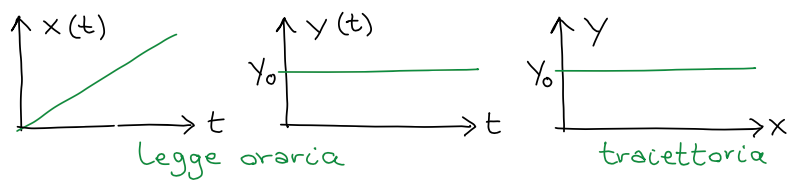
\includegraphics[width=0.8\textwidth]{images/ess-traiettoria.png}
    \end{figure}
\end{example}

\begin{definition}
    La \textbf{velocità istantanea} è la derivata della posizione rispetto al tempo.
    $$v = \lim_{\Delta t \to 0}\frac{\Delta s}{\Delta t} = \frac{ds}{dt}$$
\end{definition}

\begin{definition}
    La \textbf{velocità media} è definita come il rapporto tra lo spostamento e l'intervallo di tempo necessario per effettuarlo.
    $$v_m = \frac{\Delta s}{\Delta t}$$
\end{definition}
\hspace{-15pt}In parole povere è una grandezza che ci dice con quale rapidità cambia la posizione di un punto rispetto al tempo nell'instante $t$.
\subsection*{Vettore velocità}
Derivata rispetto al tempo del vettore posizione e si indica come 
$\frac{d\vec{r}(t)}{dt}\text{ oppure }\dot{\vec{r}}(t)[m/s]$
\begin{equation}
    \begin{split}
    \dot{\vec{r}}(t) & = (\dot{x}(t), \dot{y}(t), \dot{z}(t)) \\
     & = \frac{d}{dt}[x(t)\hat{x} + y(t)\hat{y} + z(t)\hat{z}] \\
     & = \dot{x}(t)\hat{x} + \dot{y}(t)\hat{y} + \dot{z}(t)\hat{z}
    \end{split}
\end{equation}
Per ricavare la forma esplicita uso le proprietà delle derivate (\textbf{linearità}, \textbf{Leibnitz})
\begin{example}
    $\vec{r}(t) = (v_0t, y_0, 0) = v_0t\hat{x} + y_0\hat{y}$ \:\:\:abbiamo che \:\:\:
    $\dot{\vec{r}}(t) = (v_0, 0, 0) = v_0 \hat{x}$
\end{example}
\hspace{-15pt}Velocità e spazio percorso ("integrale di linea").\\
\begin{wrapfigure}[3]{l}{5cm}
    \centering
    \includegraphics[width=5cm]{images/vettore-velocità.png}
\end{wrapfigure}
\begin{align*}
    L & = ||\vec{r}(t_1) - \vec{r}(t_0)|| + ||\vec{r}(t_2) - \vec{r}(t_1)|| + ||\vec{r}(t_3) - \vec{r}(t_2)|| + \dots \\
    & = \sum_i ||\vec{r}(t_{i+1} - \vec{r}(t_i)|| \:\: per\:\: |t_{i+1} - t_i| \text{"piccolo"} \\
    & = \sum_i ||\frac{\vec{r}(t_{i+1}) - \vec{r}(t_i)}{t_{i+1} - t_i}|| (t_{i+1} - t_i) = \int_{t_{in}}^{t_{f_{in}}}||\dot{\vec{r}}(t)||\\
\end{align*}
\begin{example}
    $\vec{r}(t) = (v_0t, y_0)\:\:\: \dot{\vec{r}}(t) = (v_0, 0)$\hspace{15pt}
    $||\dot{\vec{r}}(t)|| = \sqrt{v_0^2 + 0^2} = |v_0|$ \:\:\: $L = |v_0| \cdot (t_{f_{in}} - t_{in})$\\
    Il vettore è costante quindi facendo la derivata torna zero. Con la velocità si calcolo lo spazio percorso ("integrale di linea").
    La differenza fra le posizioni e la differenza dei tempi è il rapporto incrementale in caso gli intervalli siano sufficentemente
    piccoli, da qui si ottiene l'integrale.
\end{example}

\subsection{Vettore accelerazione}
Derivata rispetto al tempo del vettore velocità e si indica con $\frac{d^2\vec{r}(t)}{dt} \text{ oppure } \ddot{\vec{r}}(t) [m/s^2]$
\begin{equation}
    \ddot{\vec{r}}(t) = (\ddot{x}(t), \ddot{y}(t), \ddot{z}(t))\:\: = \:\: \ddot{x}(t)\hat{x} + \ddot{y}(t)\hat{y} + \ddot{z}(t)\hat{z}
\end{equation}
\begin{example}
    $\vec{r}(t)= (\frac{1}{2}a_0t^2, v_0t, 0)$ \hspace{10pt} $\dot{\vec{r}}(t) = (a_0t, v_0, 0)$ \hspace{10pt} $\dot{\vec{r}}(t) = (a_0, 0, 0)$
\end{example}
\hspace{-15pt}Serve perché l'equazione "del moto" di Newton che determinata la legge oraria è formulata in termini di accelerazione.

\subsection{Vettore quantità di moto}
Il prodotto di massa [kg] e velocità [m/s]
$$\vec{p}(t) = m \cdot \dot{\vec{r}}(t) = (m\dot{x}(t), m\dot{y}(t), m\dot{x}(t)) = m\dot{\vec{x}}(t)x + m\dot{\vec{y}}(t)y + m \dot{\vec{z}}(t)z$$
\begin{example}
    Prendiamo un punto di massa 2kg e velocità 3m/s lungo $\hat{x}$.\\
    $p_x(t) = 2 \cdot 3 kg\cdot m/s = 6 kg \cdot m/s$ \hspace{15pt} $p_y(t) = p_z(t) = 0$.
\end{example}
\hspace{-15pt}Serve per generalizzare l'equazione di Newton e per trattare sistemi di piu punti materiali.

\subsection{Vettore momento angolare rispetto a un polo P}
$$\vec{L}_p(t) = m(\vec{r}(t) - \vec{r}_p) \times \dot{\vec{r}}(t)$$
Dove $\vec{r}_p$ è il vettore posizione di p, mentre $\dot{\vec{r}}(t)$ è il prodotto vettoriale.
\begin{example}
    $\vec{r}_p = (l_0, 0, 0)$ \hspace{15pt} $\vec{r}(t) = (v_0t, y_0, 0)$\\
    $\vec{L}_p = m[(v_0t - l_0)\hat{x} + y_0\hat{y}] \times (v_0\hat{x}) \:\: = \:\: m(v_0t - l_0)v_0 \hat{x} \times \hat{x} + my_0v_0\hat{y}\times \hat{x} 
    \:\: = \:\: my_0v_0(-\hat{z}) = (0,0, -my_0v_0)$\\
    Ricorda che $\hat{x} \times \hat{x} = 0$ e $\hat{y} \times \hat{x} = -\hat{z}$
\end{example}
\hspace{-15pt}Il momento angolare dice quanta inerzia ha un oggetto in una rotazione (descrizione sommaria).\\
Il polo P è parte della definizione. È una scelta! Il risultato dipende dal polo.
Serve per formulare l'equazione del moto di sistemi di punti materiali e corpi rigidi.

\subsection{Coordinate polari}
Un metodo per rapprensentare delle cordinate x, y andando a misurare prima la distanza dall'origine e poi si va a vedere
quanto vale l'angolo fra questo segmento dall'asse x, utilizzando seno e coseno.
\begin{wrapfigure}[7]{l}{2cm}
    \centering
    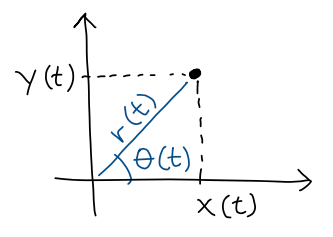
\includegraphics[width=5.5cm]{images/coordinate-polari.png}
\end{wrapfigure}
\begin{align*}
    \begin{cases}
        x(t) = r(t) \cdot \cos(\Theta(t))\\
        y(t) = r(t) \cdot \sin(\Theta(t)) 
    \end{cases}
\end{align*}
\begin{align*}
    \begin{cases}
        r(t) = \sqrt{x(t)^2 + y(t)^2} \geq 0\\
        tg(\Theta(t)) = y(t) / x(t) 
    \end{cases}
\end{align*}
\\
\begin{example} Esempi di rappresentazione di coordinate in coordinate polari.\\
    $x = 0, y = l_0 > 0 \:\: \Rightarrow \:\: r = l_0, \Theta = \pi/2$\\
    $x = 0, y = -l_0 < 0 \:\: \Rightarrow \:\: r = l_0, \Theta = -\pi/2$\\
    $x = l_0, y = l_0 > 0 \:\: \Rightarrow \:\: r = \sqrt{2}l_0, \Theta = \pi/4$\\
\end{example}

\subsection{Versori polari (2D)}
Definisco un versore $\hat{r}(t)$ che punta verso il punto materiale e un versore $\hat{\Theta}(t)$ ortogonale.
Si esprime facilmente in coordinte polari.
$$\vec{r}(t) = (x(t), y(t)) = (r(t)\cos \Theta(t), r(t)\sin\Theta(t)) \:\: = \:\: r(t)(\cos\Theta(t)\hat{x} + \sin\Theta(t)\hat{y})$$
Ma $||\vec{r}(t)|| = |r(t)| = r(t)$ allora definisco $\hat{r}(t) = \vec{r}(t)/ ||\vec{r}(t)|| = \cos \Theta(t)\hat{x} + \sin\Theta(t)\hat{y}$\\\\
Trovo facilmente che un versore ortogonale è:
$$\hat{\Theta(t)} = -\sin\Theta(t)\hat{x} + \cos\Theta(t)\hat{y} \:\:\:\text{infatti} \:\:\: \hat{r}\cdot \hat{\Theta} = c \cdot (-s) + s \cdot c = 0$$
\begin{wrapfigure}[7]{r}{6cm}
    \centering
    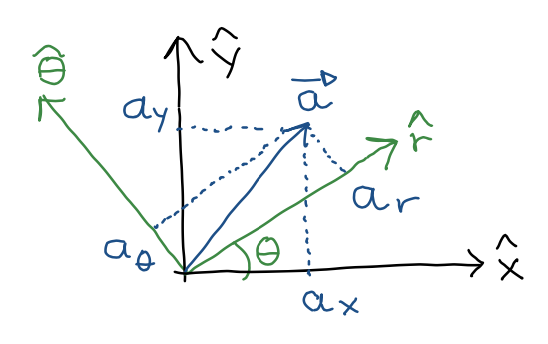
\includegraphics[width=5.5cm]{images/trasformazioni-inverse.png}
\end{wrapfigure}
\begin{note}
    Non c'è legame fra $\Theta$ e $\hat{\Theta}$ è solo una convenzione.
\end{note}
\hspace{-15pt}Le trasformazioni inverse invece si fanno come segue (verifico per sostituzione):
$$\hat{y} = \cos\Theta(t)\hat{r} - \sin\Theta(t)\hat{\Theta} \hspace{20pt} \hat{y} = \sin\Theta(t)\hat{r} + \cos\Theta(t)\hat{\Theta}$$
Possono quindi scrivere ogni vettore nella forma $\vec{a} = a_r\hat{r} + a_{\Theta}\hat{\Theta}$ con le componenti polari $a_r, a_{\Theta}$.
Per evitare ambiguità non scriviamo $(a_r, a_{\Theta})$ e riserviamo la notazione alle componenti cartesiane.\\\\
A differenza dei versori cartesiani quelli polari dipendono dal tempo per costruzioni.
$$\dot{\hat{r}}(t) = \frac{d}{dt}[\cos\Theta(t) \hat{x} + \sin\Theta(t)\hat{y}] \:\: = \:\: -\sin\Theta(t) \cdot \dot{\Theta}(t)\hat{x} + \cos\Theta(t) \cdot \dot{\Theta}(t)\hat{y}$$
Dove $\cos\Theta(t) \cdot \dot{\Theta}(t)$ si applica la derivata della somma, Leibnitz, funzione composta.
$$= \dot{\Theta}(t)\cdot \hat{\Theta}(t) \:\:\:\:(\text{confronto l'espressione di} \hat{\Theta}(t))$$
Similmente $\dot{\hat{\Theta}}(t)= - \dot{\Theta}\hat{r}(t)$.


\subsection*{Vettori posizione, velocità, accelerazione}
$$\vec{r}(t) = r(t)\hat{r}(t)$$
Dove abbiamo che $\vec{r}(t)$ è il vettore, $r(t)$ è una coordinata polare, $\hat{t}(t)$ è il versore polare.
$$\dot{\vec{r}}(r) = \dot{r}(t)\hat{r}(t) + r(t)\dot{\Theta}(t)\hat{\Theta}(t)$$
Dove la parte $\dot{\vec{r}}(r)$ è la velocità radiale.
$$\ddot{\vec{r}}(t) = [\ddot{r}(t) - r(t)\dot{\Theta}(t)^2] \hat{r} + [r(t) \ddot{\Theta}(t) + 2\dot{r}(t)\dot{\Theta}(t)]\hat{\Theta}$$
Nel quale abbiamo che la parte $r(t)\dot{\Theta}(t)^2$ si chiama \textbf{velocità centripeta}, mentre $2\dot{r}(t)\dot{\Theta}(t)$ si dice \textbf{accelerazione di Coriolis}.


	% !TeX spellcheck = it_IT
\newpage
\section{Modelli di dati}
Progettare una BD significa progettare la struttura dei dati e le applicazioni. Per farlo al meglio è fondamentale rappresentare in modo \textbf{astratto} e simbolico il dominio del discorso tramite la \textbf{modellazione}.
\begin{definition}[Modello astratto]
	Un modello astratto è la \textbf{rappresentazione formale} di idee e conoscenze relative ad un fenomeno tramite un \textbf{linguaggio formale} a seguito di una \textbf{interpretazione} soggettiva.
\end{definition}

\subsection{Ruoli}
I ruoli principali nella modellazione sono:
\begin{itemize}
	\item \textbf{Committente}: persona con l'esigenza
	\item \textbf{Progettista} o \textbf{analista}: crea un progetto concettuale
	\item \textbf{Programmatore}: sviluppano la BD e le applicazioni
	\item \textbf{DB Administrator}: gestisce gli utenti e il sistema
\end{itemize}

\subsection{Fasi}
Le fasi della progettazione sono:
\begin{enumerate}
	\item \textbf{Analisi dei requisiti}: definizione dei bisogni del committente
	\item \textbf{Progettazione concettuale}: traduzione dei requisiti in un progetto, struttura concettuale dei dati, dei vincoli e delle operazioni
	\item \textbf{Progettazione logica}: traduzione dello \textit{schema concettuale} nello schema logico, che è espresso nel modello dei dati del sistema scelto
	\item \textbf{Progettazione fisica}: produce lo schema fisico che arricchisce quello logico con specifiche sull'organizzazione fisica dei dati
\end{enumerate}

\begin{center}
	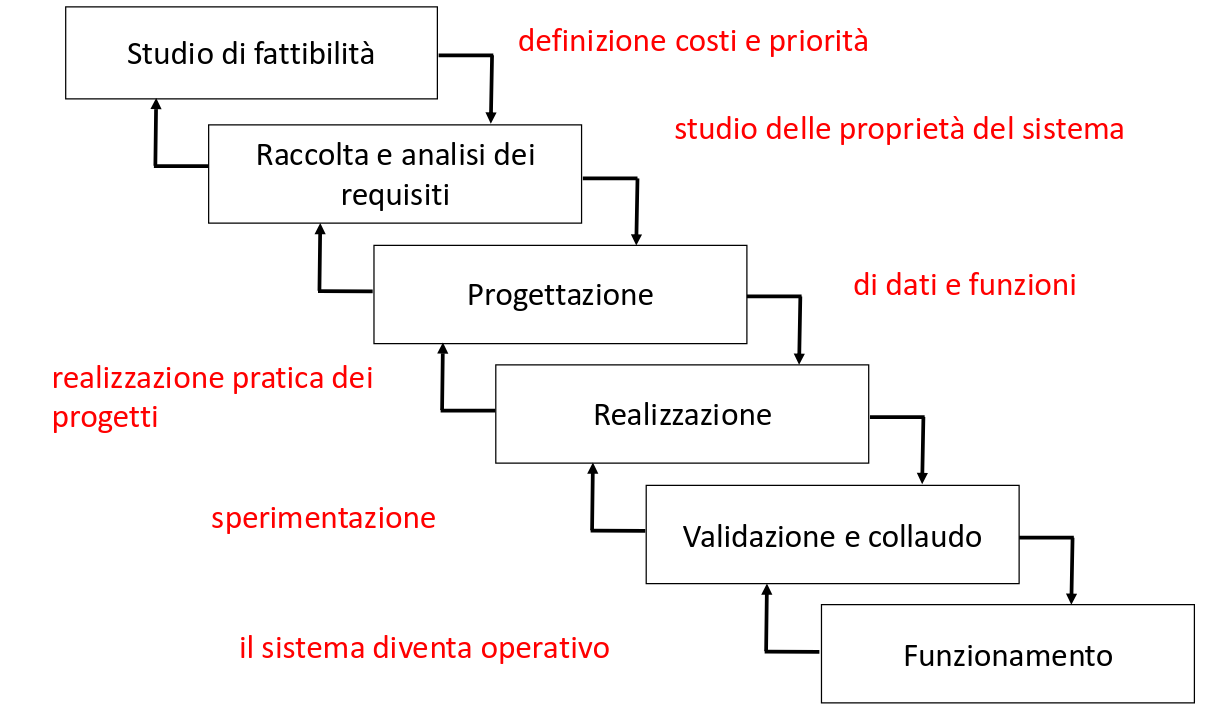
\includegraphics[scale=0.3]{fasi_prog.png}
\end{center}

\subsection{Aspetto ontologico}
Questo aspetto si concentra su quale conoscenza del dominio deve essere rappresentata. In particolare la conoscenza può essere \textbf{astratta}, \textbf{concreta} o \textbf{procedurale} (operazioni di base e comunicazione). 

\subsubsection{Conoscenza concreta}
La conoscenza concreta riguarda i \textbf{fatti} specifici che si vogliono rappresentare: \textbf{entità}, \textbf{collezioni} e \textbf{associazioni}.

\paragraph{Entità e proprietà}
Le \textbf{entità} sono ciò di cui ci interessa rappresentare alcuni fatti o proprietà (e.g. un libro) mentre le \textbf{proprietà} sono fatti che descrivono caratteristiche di determinate entità (e.g. titolo).

\begin{note}
	Un'entità non coincide con l'insieme dei valori assunti dalle sue proprietà, in quanto queste possono cambiare nel tempo o possono essere identiche pur essendo due entità diverse. E.g. una persona la cui età aumenta ogni anno o due persone con stesso nome, età e indirizzo.
\end{note}

Una \textbf{proprietà} è una coppia \textit{nome} e \textit{valore}, dove quest'ultimo è di un certo tipo e all'interno di un \textbf{dominio} di possibili valori. Si possono classificare come:
\begin{itemize}
	\item \textbf{Atomica} se il suo valore non è scomponibile, altrimenti \textbf{strutturata}
	\item \textbf{Univoca} se il suo valore è unico, altrimenti \textbf{multivalore}
	\item \textbf{Totale} o \textbf{obbligatoria} se ogni entità nell'universo assume un valore per essa, altrimenti \textbf{parziale} o \textbf{opzionale}
	\item \textbf{Costante} o \textbf{variabile}
	\item \textbf{Calcolata} o \textbf{non calcolata}
\end{itemize}

Un \textbf{tipo di entità} è una descrizione astratta di ciò che accomuna un insieme di entità omogenee, esistenti o possibili. È quindi un insieme infinito. E.g. persona, auto, esame.

\paragraph{Collezione}
Una collezione è un insieme \textbf{variabile} nel tempo di entità omogenee interessanti nel dominio. L'insieme degli elementi di una collezione in un dato momento è detto \textbf{estensione} della collezione. A differenza del \textit{tipo di entità}, questi insiemi sono finiti.

\paragraph{Associazione}

\begin{definition}[Istanza di associazione]
	Un'\textbf{istanza di associazione} è un fatto che correla due o più entità stabilendo un legame logico tra di loro. 
\end{definition}

\begin{definition}[Associazione]
	L'\textbf{associazione} $R(X,Y)$ fra due collezioni di entità $X$ e $Y$ è quindi l'insieme di istanze di associazione tra gli elementi di $X$ e $Y$ che varia nel tempo.
\end{definition}

\begin{definition}[Prodotto cartesiano]
	Il \textbf{prodotto cartesiano} $(X \times Y)$ è il dominio dell'associazione.
\end{definition}

\begin{observation}
	Se vediamo due collezioni $X$ e $Y$ come due insiemi, un’istanza di associazione tra di loro può essere vista come una coppia di elementi $(x; y)$, con $x \in X$ e $y\in Y$, e quindi un’associazione $R$ tra $X$ e $Y$ può essere vista come un sottoinsieme del prodotto $X \times Y$, ovvero come	una relazione matematica tra tali insiemi.
\end{observation}

\noindent Le associazioni hanno due caratteristiche strutturali:
\begin{itemize}
	\item \textbf{Molteplicità}
	\begin{definition}[Vincolo di univocità]
		Un’associazione $R(X, Y)$ è \textbf{univoca} rispetto ad $X$ se per ogni elemento $x \in X$ esiste al più un elemento di $Y$ che è associato ad $x$. Altrimenti è \textbf{multivalore} rispetto ad $X$.
	\end{definition}
	Questo ci porta alla \textbf{cardinalità} di un'associazione, che può essere:
	\begin{itemize}
		\item \textbf{Uno a molti}: $R(X,Y)$ è $(1:N)$ se essa è multivalore su $X$ ed univoca su $Y$
		\begin{center}
			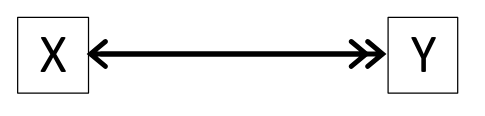
\includegraphics[scale=0.2]{unomolti.png}
		\end{center}
		\item \textbf{Molti a uno}: $R(X,Y)$ è $(N:1)$ se essa è univoca su $X$ e multivalore
		\begin{center}
			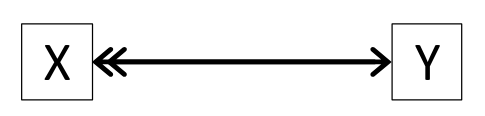
\includegraphics[scale=0.2]{moltiuno.png}
		\end{center}
		\item \textbf{Molti a molti}: $R(X,Y)$ è $(N:M)$ se essa è multivalore su $X$ e $Y$
		\begin{center}
			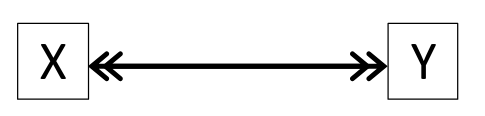
\includegraphics[scale=0.2]{moltimolti.png}
		\end{center}
		\item \textbf{Uno a uno}: $R(X,Y)$ è $(1:1)$ se essa è univoca su $X$ e $Y$
		\begin{center}
			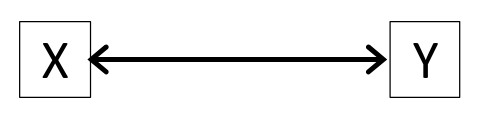
\includegraphics[scale=0.2]{unouno.png}
		\end{center}
	\end{itemize}
	\item \textbf{Totalità}
	\begin{definition}[Vincolo di totalità]
		Un’associazione $R(X, Y)$ è \textbf{totale} (o surgettiva) su $X$ se per ogni elemento $x \in X$ esiste almeno un elemento di $Y$ che è associato ad $x$. Altrimenti è \textbf{parziale} rispetto ad $X$.
	\end{definition}
	\begin{figure}[!h]
		\centering
		\begin{minipage}[b]{0.2\textwidth}
			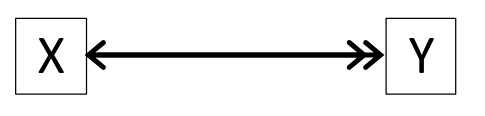
\includegraphics[width=\textwidth]{totale.png}
			\caption*{Totale}
		\end{minipage}
		\hspace{30pt}
		\begin{minipage}[b]{0.2\textwidth}
			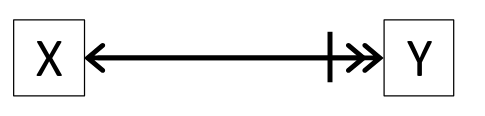
\includegraphics[width=\textwidth]{parziale.png}
			\caption*{Parziale}
		\end{minipage}
	\end{figure}
\end{itemize}

Un'associazione si rappresenta come visto e con l'aggiunta di un'\textbf{etichetta} con il suo nome, scelto di solito con un \textit{predicato}.

\subsubsection{Conoscenza astratta}
La conoscenza astratta riguarda i fatti generali che descrivono la \textbf{struttura} della conoscenza concreta, le \textbf{restrizioni} sui valori possibili della conoscenza concreta e sui \textbf{vincoli d'integrità} e le \textbf{regole} per dedurre nuovi fatti.

\begin{definition}[Modello dei dati]
	Un modello dei dati è un insieme di meccanismi di astrazione per descrivere la struttura della conoscenza concreta.
\end{definition}

\begin{definition}[Schema]
	Uno schema è la descrizione della struttura della conoscenza concreta e dei vincoli di integrità usando un particolare modello di dati.
\end{definition}

\begin{note}
	Come notazione grafica per lo schema usiamo una \textbf{variante} del modello ER.
\end{note}

\paragraph{Oggetti}
Ad ogni \textbf{entità} del dominio corrisponde un oggetto che può rispondere a dei \textbf{messaggi} (anche chiamati \textbf{attributi}), restituendo valori memorizzati o calcolati tramite procedure.

\begin{definition}[Oggetto]
	Un oggetto è un’entità software che	modella un’entità dell’universo e che ha:
	\begin{itemize}
		\item \textbf{Stato}: modellato da un insieme di costanti o variabili con valori di qualsiasi complessità
		\item \textbf{Comportamento}: un insieme di procedure locali chiamate \textbf{metodi}, che modellano le operazioni di base che riguardano l’oggetto e le proprietà	derivabili da altre
		\item \textbf{Identità}
	\end{itemize}
\end{definition}

\noindent Il \textbf{tipo oggetto} definisce l'insieme dei messaggi a cui può rispondere un insieme di possibili oggetti. Tra i tipi oggetto può essere definita una \textbf{relazione di sottotipo} che ha le seguenti proprietà:
\begin{itemize}
	\item È \textbf{asimmetrica}, \textbf{riflessiva} e \textbf{transitiva} (relazione di \textit{ordine parziale})
	\item \textbf{Sostitutività}: se $T$ è sottotipo di $T'$ allora gli elementi di $T$ possono essere usati in ogni contesto i cui possano apparire quelli di $T'$. In particolare:
	\begin{itemize}
		\item Gli elementi di $T$ hanno tutte le \textbf{proprietà} di quelli di $T'$
		\item Per ogni \textbf{proprietà} $p \in T'$, il suo tipo $T$ è un sottotipo del suo tipo in $T'$
	\end{itemize}
\end{itemize}

\paragraph{Classe}
Una classe è un insieme di oggetti dello stesso tipo, modificabile con operatori per includere o estrarre elementi dall'insieme.\\
Spesso le classi sono organizzate in una \textbf{gerarchia} di \textbf{specializzazione} o \textbf{generalizzazione} (\textbf{sottoclassi} e \textbf{superclassi}). Queste hanno due caratteristiche:
\begin{itemize}
	\item \textbf{Ereditarietà} delle proprietà che permette di definire:
	\begin{itemize}
		\item un tipo oggetto a partire da un altro
		\item l'implementazione di un tipo oggetto a partire da un'altra implementazione. In questo caso gli attributi possono solo essere \textbf{aggiunti} o \textbf{ridefiniti} solo specializzandone il tipo
	\end{itemize}
	\item Gli elementi di una sottoclasse sono un \textbf{sottoinsieme} di quelli della superclasse. Questa relazione ha le seguenti proprietà:
	\begin{itemize}
		\item È \textbf{asimmetrica}, \textbf{riflessiva} e \textbf{transitiva}
		\item \textbf{Vincolo intensionale}: se $C$ è sottoclasse di $C'$ allora il tipo degli elementi di $C$ è sottotipo degli elementi di $C'$
		\item \textbf{Vincolo estensionale}: se $C$ è sottoclasse di $C'$ allora gli elementi di $C$ sono un sottoinsieme degli elementi di $C'$
	\end{itemize}
\end{itemize}

I vincoli sugli insieme di sottoclassi possono essere di \textbf{disgiunzione} e di \textbf{copertura}. Questo porta ad avere quattro tipi di relazioni tra sottoinsiemi:
\begin{itemize}
	\item \textbf{Scorrelate}: non richiedono nessun vincolo e possono essere rappresentate in due modi
	\begin{center}
		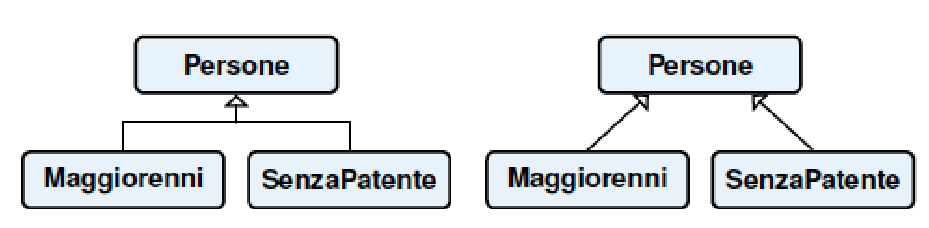
\includegraphics[scale=0.2]{scorrelate.png}
	\end{center}
	\item \textbf{Disgiunte}
	\begin{center}
		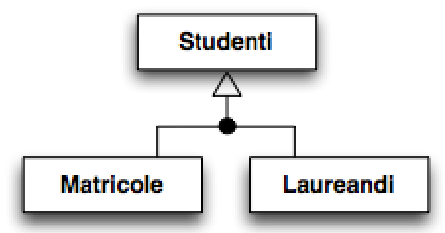
\includegraphics[scale=0.2]{disgiunte.png}
	\end{center}
	\item \textbf{Copertura}
	\begin{center}
		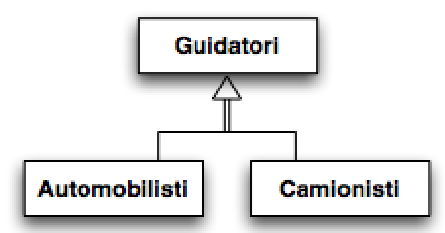
\includegraphics[scale=0.2]{copertura.png}
	\end{center}
	\item \textbf{Partizione}
	\begin{center}
		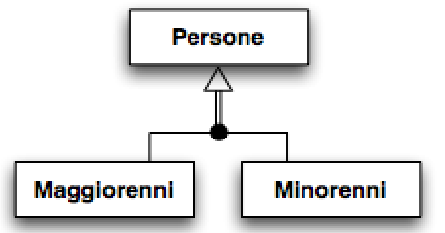
\includegraphics[scale=0.2]{partizione.png}
	\end{center}
\end{itemize}

È possibile avere l'\textbf{ereditarietà multipla} definendo un tipo per ereditarietà da più supertipi. Bisogna prestare attenzione quando un attributo viene ereditato da più antenati.

\paragraph{Associazioni}
Le associazioni si modellano con un costrutto apposito e possono avere delle \textbf{proprietà} ed essere \textbf{ricorsive}. L'ultimo caso si presenta quando abbiamo relazioni binarie fra gli elementi di una stessa collezione. In questo caso bisogna etichettare anche i ruoli agli estremi della freccia.
\begin{center}
	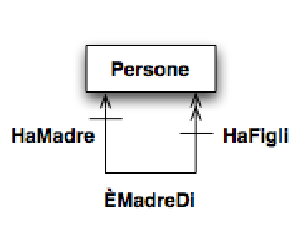
\includegraphics[scale=0.4]{ass_ric.png}
\end{center}
\begin{note}
	È possibile avere più associazioni tra classi diverse che rappresentano informazioni diverse.
\end{note}

\begin{observation}[Reificazione]
	È possibile trasformare un'associazione tra due classi in una situazione con tre classi e due associazioni. Ad esempio:
	\begin{center}
		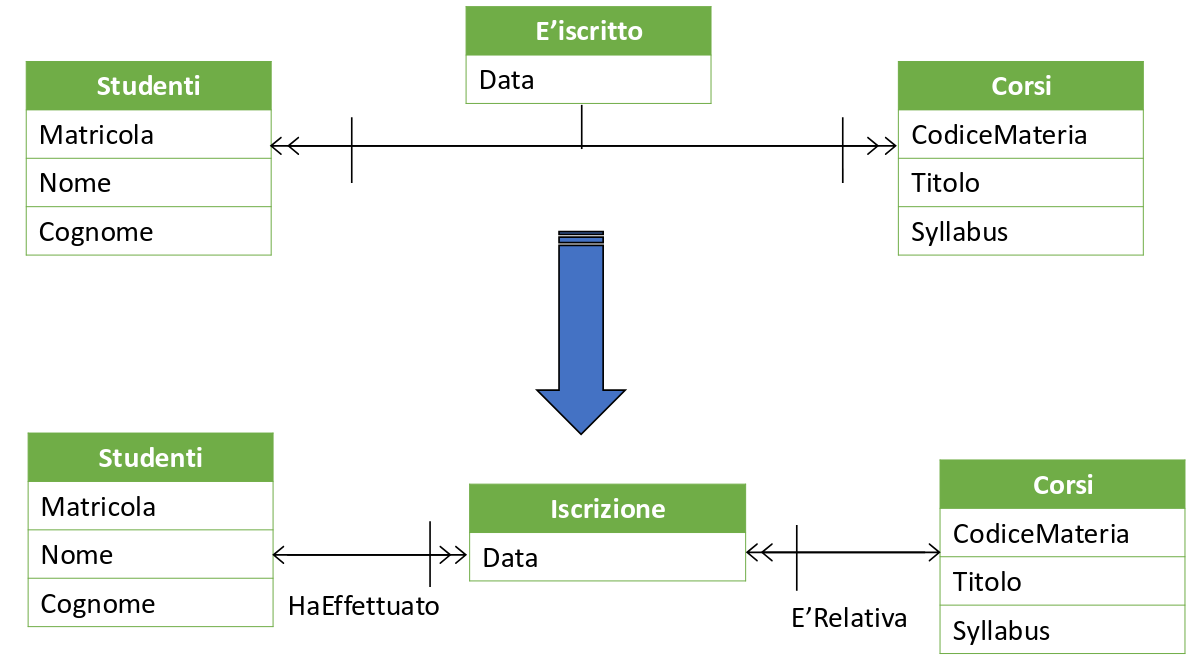
\includegraphics[scale=0.3]{reificazione.png}
	\end{center}
\end{observation}

\paragraph{Restrizioni}
I \textbf{vincoli d'integrità} impongono restrizioni sui possibili valori della conoscenza concreta. Possono essere \textbf{statici} o \textbf{dinamici} e arricchiscono la descrizione di una classe.
\begin{center}
	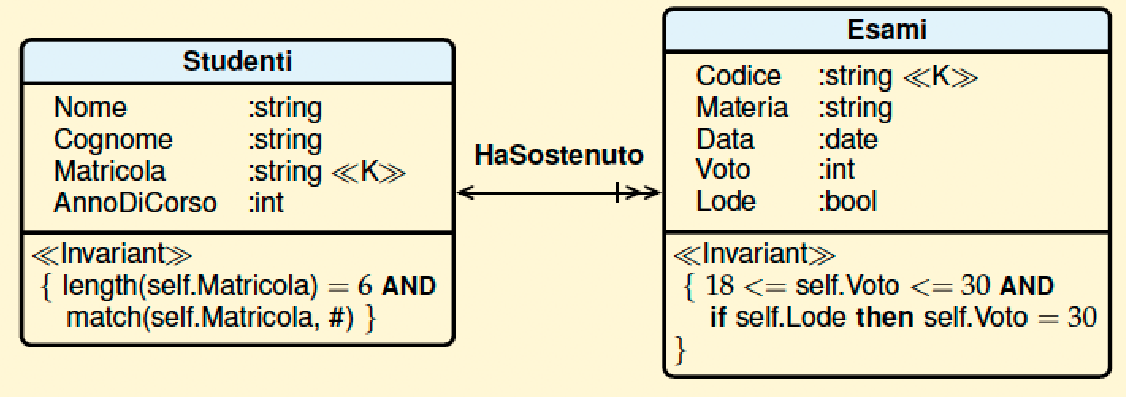
\includegraphics[scale=0.3]{vincoli.png}
\end{center}

\begin{note}
	Gli attributi marcati con $<<K>>$ sono una \textbf{chiave}.
\end{note}

\subsection{Modello entità-relazione}
È Il modello più popolare per il disegno concettuale di BD. Non tratta gerarchie di inclusione tra collezioni, non distingue collezioni e tipi e non supporta alcun meccanismo di ereditarietà. Definisce un meccanismo per modellare direttamente le associazioni non binarie o con proprietà.\\
Prevede due meccanismi di \textbf{astrazione}:
\begin{itemize}
	\item Modellare \textbf{insiemi di entità}, con le relative proprietà
	\item Modellare le associazioni (chiamate \textbf{relazioni}).
\end{itemize}
Le collezioni sono chiamate \textbf{tipi di entità}, e gli attributi dei loro elementi possono assumere solo valori di tipo primitivo.
\begin{center}
	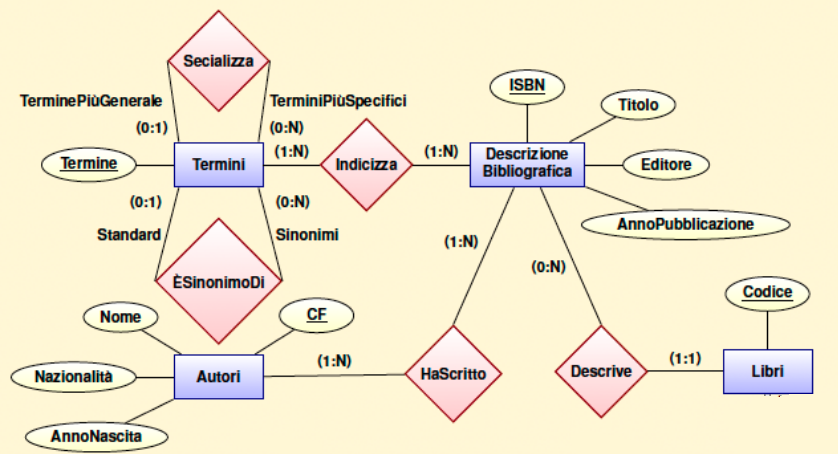
\includegraphics[scale=0.5]{entita_relazione.png}
\end{center}
\subsection{Modello relazionale}
E’ il modello dei dati usato dagli attuali sistemi commerciali. I meccanismi per definire una base di dati con questo modello sono l’\textbf{ennupla} e la \textbf{relazione}.

\begin{definition}[Ennupla]
	Un tipo ennupla è un insieme di coppie (attributo, tipo primitivo) ed un valore di tipo	ennupla è un insieme di coppie (attributo, valore), dette anche campi, con gli stessi attributi del tipo e in cui il valore di ogni attributo appartiene al corrispondente tipo	primitive.
\end{definition}

\begin{definition}[Relazione]
	Una relazione è un insieme di ennuple con lo stesso tipo.
\end{definition}

\begin{definition}[Superchiave e chiave]
	Un insieme di attributi i cui valori determinano univocamente un’ennupla di una	relazione $R$ è una \textbf{superchiave} per $R$. Una superchiave tale che togliendo un qualunque attributo essa non sia più una	superchiave è una \textbf{chiave} per $R$. Tra le chiavi di $R$ ne viene scelta una come chiave \textbf{primaria}.
\end{definition}
Le \textbf{associazioni} tra i dati sono rappresentate attraverso opportuni attributi, chiamati \textbf{chiavi esterne}, che assumono come valori quelli della chiave primaria di un’altra relazione. 

\begin{center}
	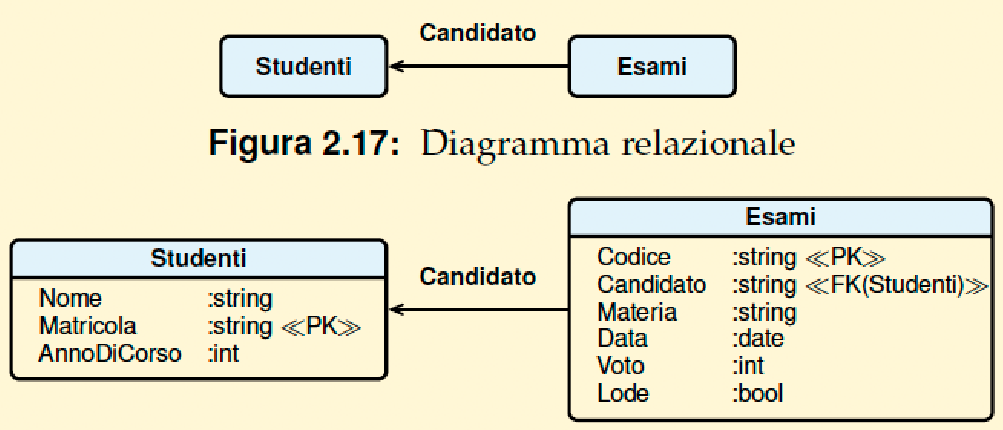
\includegraphics[scale=0.4]{mod_rel.png}
\end{center}
	% !TeX spellcheck = it_IT
\newpage
\section{Progettazione}
La fase di progettazione è tra quella della specifica (cosa fare) e quella della programmazione. Come risultato produce un'\textbf{architettura} che descrive \textbf{come} fare.\\
Possono esserci due livelli di astrazione:
\begin{itemize}
	\item \textbf{Architetturale}: si scompone un sistema in più sottosistemi, ne si identificano e specificano le parti e le interconnessioni
	\item Di \textbf{dettaglio}: indica come la specifica di ogni parte sarà realizzata
\end{itemize}

\begin{definition}[Architettura software]
	L’architettura di un sistema software è la \textbf{struttura} del sistema, costituita dalle parti del sistema, dalle \textbf{relazioni} tra le parti e dalle loro proprietà visibili.
\end{definition}

\begin{definition}[Stile architetturale]
	Uno stile architetturale caratterizza una famiglia di architetture con caratteristiche simili (e.g. client-server, microservizi). Le funzionalità e le interazioni tra i componenti spesso seguono degli standard.
\end{definition}

Un'architettura si sviluppa in diverse \textbf{viste} e \textbf{stili}.

\subsection{Vista comportamentale}
Anche detta \textbf{component-and-connector}, descrive un sistema software come \textbf{composizione di componenti}, compreso di:
\begin{itemize}
	\item \textbf{Interfacce} dei componenti
	\item Caratteristiche dei \textbf{connettori}
	\item Struttura del sistema in esecuzione (flusso dei dati, parallelismo, replicazioni, etc..)
\end{itemize}
Questa vista permette l'analisi delle \textbf{caratteristiche di qualità} a tempo di esecuzione (prestazioni, affidabilità, etc..) e di documentare lo \textbf{stile} dell'architettura.

\subsubsection{Componente}
Una componente software è un'unità concettuale di decomposizione del sistema a tempo di esecuzione. Incapsula un insieme di \textbf{funzionalità} e/o \textbf{dati}, restringendone l'accesso tramite delle \textbf{interfacce}.
\begin{definition}[Componente]
	Una componente software è un'unità di software \textbf{indipendente} e \textbf{riutilizzabile}.
\end{definition}

\begin{definition}[Sistema software]
	Un sistema software è una composizione di componenti software basata sulla connessione di più componenti e realizzata con interfacce dei componenti e connettori,
\end{definition}

\noindent In UML un componente è un \textbf{classificatore} e si compone di:
\paragraph{Porti} I porti ne identificano i punti di interazione. Può essercene più di uno, possono fornire o richiedere una o più \textit{interfacce} e possono avere \textit{nomi} e \textit{molteplicità}.
\begin{center}
	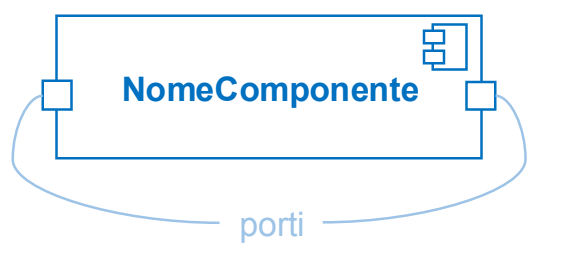
\includegraphics[scale=0.3]{component.png}
\end{center}
I porti possono avere la specifica delle interfacce in due modi:
\begin{itemize}
	\item \textbf{Sintetica}: si indica solo quando è \textit{richiesta} (forchetta) o offerta (\textit{lollipop})
	\begin{center}
		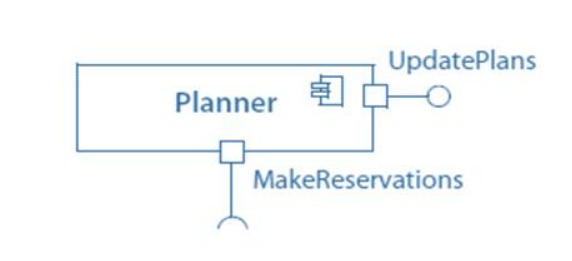
\includegraphics[scale=0.2]{interfaccia_sintetica.png}
	\end{center}
	\item \textbf{Estesa}: si specifica per esteso le operazioni richieste ed offerte
	\begin{center}
		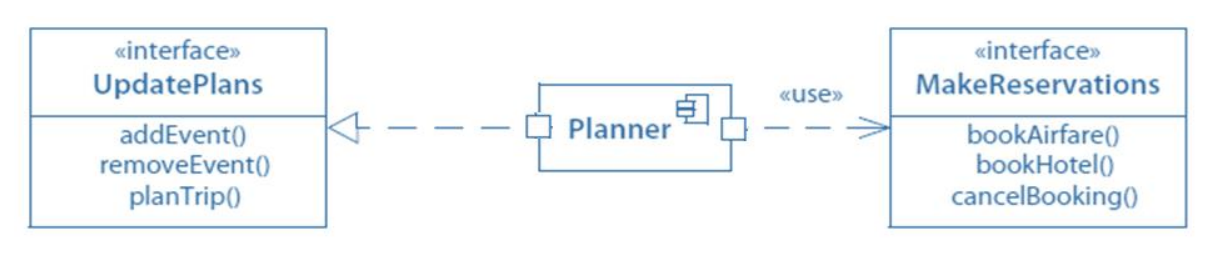
\includegraphics[scale=0.2]{interfaccia_estesa.png}
	\end{center}
\end{itemize}

\paragraph{Connettori}
I connettori sono \textbf{canali di interazione} tra i porti di componenti. Non hanno un descrittore specifico e vengono rappresentati come associazioni. Per dare più informazioni si indica lo \textbf{stile} della connessione o con uno \textbf{stereotipo} o indicando i \textbf{ruoli}.

\begin{center}
	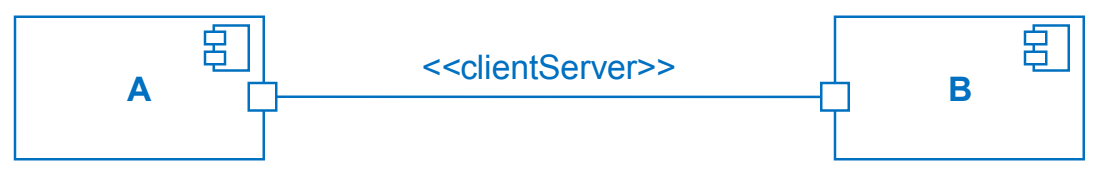
\includegraphics[scale=0.3]{connettori.png}
\end{center}

\subsubsection{Stili}
In questo tipo di vista uno stile architetturale è caratterizzato dalle \textbf{caratteristiche generali} delle componenti e dalle loro \textbf{interazioni} (quindi \textit{porti} e \textit{connettori}).

\paragraph{Pipes \& filters} Questo stile consiste in un flusso di elaborazione di dati che viaggiano lungo le \textbf{pipe} e sono processati dai \textbf{filter}. In particolare i \textit{filter} sono i \textbf{componenti} che trasformano i flussi di dati mentre le \textit{pipe} sono i \textbf{connettori} che fungono da canale di comunicazione unidirezionale bufferizzato che preserva l'ordine di ingresso.
\begin{center}
	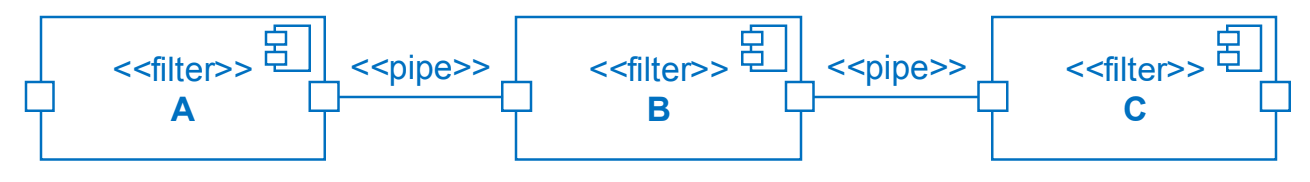
\includegraphics[scale=0.3]{pipes_filters.png}
\end{center}

\paragraph{Client-server} Questo stile prevede due componenti che possono essere su macchine diverse. Il \textbf{server} offre il servizio, aspetta le richieste dati ad un porto e può servirne su di esso più alla volta. Il \textbf{client} invia richieste al server e attende una risposta.
\begin{center}
	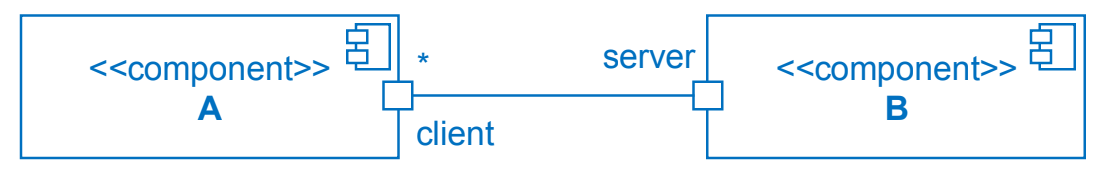
\includegraphics[scale=0.3]{client-server.png}
\end{center}
Il server in particolare prevede un \textbf{RequestListener} in attesa di richieste e un \textbf{RequestHandler} per ognuna di esse. Quest'ultimo elabora le richieste e:
\begin{itemize}
	\item Se \textbf{stateless} le gestisce ognuna in maniera indipendente
	\item Se \textbf{stateful} consente richieste \textit{composite} che consistono in più richieste \textit{atomiche}, mantenendo un record di esse \textbf{sessione}
\end{itemize}

\paragraph{Master-slave}
Questo stile è una variazione di \textit{client-server} in cui c'è solamente un servente (\textbf{slave}) e un cliente (\textbf{master})

\paragraph{Peer to Peer} Questo stile è una variazione di \textit{client-server} dove tutti i componenti sono sia client che server e avviene uno scambio di servizi alla pari.
\begin{center}
	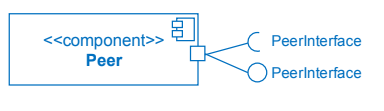
\includegraphics[scale=0.6]{p2p.png}
\end{center}

\paragraph{Publish-Subscribe} In questo stile i componenti interagiscono in modo \textbf{event-based}. Abbiamo tre tipi di componenti:
\begin{itemize}
	\item \textbf{Publisher}: produce classi di eventi
	\item \textbf{Subscriber}: si iscrive alle classi rilevanti
	\item \textbf{Broker}: smista gli eventi pubblicati
\end{itemize}
Un componente può essere sia \textit{publisher} che \textit{subscriber}. Tra di loro comunicano tramite il \textit{broker}.I publisher non sanno quanti/quali subscriber ci siano e viceversa, garantendo \textbf{scalabilità}.
Questo stile può funzionare in due modi:
\begin{itemize}
	\item \textbf{Push}: il broker invia attivamente i messaggi ai subscriber, controllandone la frequenza
	\item \textbf{Pull}: è il subscriber che manualmente recupera i messaggi dal broker. Migliora la scalabilità e la flessibilità dato che servono meno broker.
\end{itemize}

\begin{figure}[!h]
	\centering
	\begin{minipage}[b]{0.5\textwidth}
		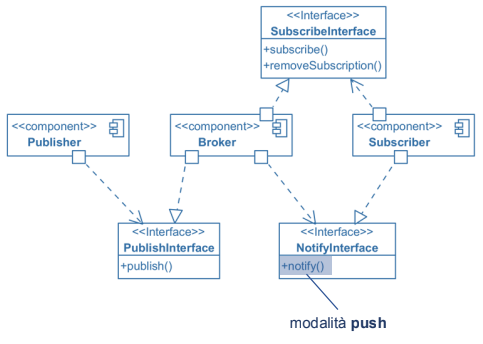
\includegraphics[width=\textwidth]{pub-sub.png}
	\end{minipage}
	\hfill
	\begin{minipage}[b]{0.4\textwidth}
		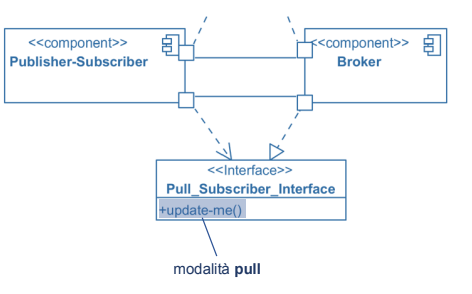
\includegraphics[width=\textwidth]{pub_sub_full.png}
	\end{minipage}
\end{figure}

\paragraph{Process coordinator}
Un componente funge da \textbf{process coordinator} mentre gli altri sono passivi e non conoscono il loro ruolo nel processo ma si limitano a contribuire. Il \textit{coordinator} conosce la sequenza di passi necessaria, invoca le funzionalità richieste e fornisce una risposta.

\newpage
\paragraph{Model-View-Controller/Publisher}
Questo stile si basa su tre elementi:
\begin{itemize}
	\item \textbf{Model}: nucleo funzionale che implementa la business logic dell'applicazione e ne rappresenta i dati su cui essa lavora
	\item \textbf{View}: presentazione del model all'utente, possono essercene diverse
	\item \textbf{Controller}: controlla l'input dell'utente e lo traduce in operazioni da eseguire su \textit{model} oppure \textbf{presenter} in alternativa
\end{itemize}
\begin{figure}[!h]
	\centering
	\begin{minipage}[b]{0.4\textwidth}
		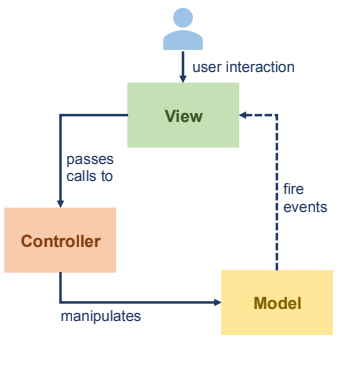
\includegraphics[width=\textwidth]{model_view_controller.png}
		\caption*{Controller}
	\end{minipage}
	\hspace{10pt}
	\begin{minipage}[b]{0.4\textwidth}
		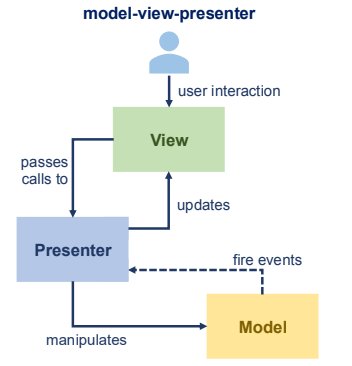
\includegraphics[width=\textwidth]{model_view_presenter.png}
		\caption*{Presenter}
	\end{minipage}
\end{figure}

\subsection{Vista strutturale}
Descrive la struttura di un sistema software come insieme di \textbf{unità di realizzazione}, ovvero di codice (e.g. classi e package). Permette di analizzare le \textbf{dipendenze}, progettare i \textbf{test} e valutare la \textbf{portabilità}.

\subsection{Vista di deployment}
Descrive l'allocazione del software su ambienti di esecuzione e permette di valutarne \textbf{prestazioni} e \textbf{affidabilità}.
	% !TeX spellcheck = it_IT
\newpage
\section{Modello relazionale}
Il modello relazionale fu presentato da E. F. Codd nel 1970 per favorire l'\textbf{indipendenza} dei dati. Si basa sul concetto di \textbf{relazione}, la quale ha come rappresentazione la \textbf{tabella}.\\
In ogni base di dati distinguiamo lo \textbf{schema relazionale}, invariato nel tempo e che descrive la struttura) e l'\textbf{istanza}, ovvero i valori attuali.

\subsection{Matematica}
In matematica definiamo una \textbf{relazione} come l'insieme dei \textbf{domini}
\begin{equation*}
	D_1, \ldots, D_n
\end{equation*}
Inoltre il \textbf{prodotto cartesiano} $D_1 \times \ldots \times D_n$è l'insieme di tutte le \textbf{n-uple} $(d_1, \ldots, d_n)$ tali che 
\begin{equation*}
	d_1 \in D_1, \ldots, d_n \in D_n
\end{equation*}

\begin{example}[Relazioni in matematica]
	Dati i domini
	\begin{equation*}
		D_1 = \{a,b\} \qquad D_2 = \{x,y,z\}
	\end{equation*}
	il prodotto cartesiano è
	\begin{equation*}
		D_1 \times D_2 = \{(a, x), (a, y), (a, z), (b, x), (b,y), (b,z)\}
	\end{equation*}
	mentre una relazione possibile è
	\begin{equation*}
		r \subseteq D_1 \times D_2 = \{(a,x),(a,z), (b,y)\}
	\end{equation*}
\end{example}

\subsection{Modello}
I meccanismi per definire una BD con il modello relazionale sono la \textbf{ennupla} (insieme finito di coppie (Attributo, Tipo elementare)) e la \textbf{relazione}.

\begin{definition}[Schema di relazione]
	Uno schema di relazione $R(T)$ è una coppia formata da un \textbf{nome} $R$ e da un \textbf{tipo} $T$ definito come segue:
	\begin{itemize}
		\item \textit{int}, \textit{real}, \textit{boolean} e \textit{string} sono tipi \textbf{primitivi}
		\item $T=(A_1:T_1, \ldots, A_n:T_n)$ è un tipo \textbf{ennupla} di \textbf{grado} $n$ se $T_1, \ldots, T_n$ sono tutti tipi primitivi e se $A_1, \ldots, A_n$ sono etichette distinte dette \textbf{attributi}
		\item Due ennuple sono uguali se hanno uguale il grado, gli attributi e il tipo degli attributi con lo stesso nome
		\item L'ordine degli attributi non importa
		\item Se $T$ è tipo ennupla allora $\{T\}$ è un insieme di ennuple o tipo \textbf{relazione}
		\item Due tipi relazione sono uguali se hanno lo stesso tipo ennupla
	\end{itemize}
\end{definition}

\begin{definition}[Schema relazionale]
	Uno schema relazionale è costituito da schemi di relazione $R_i:\{T_i\} \quad i=1, \ldots, k$ e da un insieme di relativi \textbf{vincoli di integrità}.
\end{definition}

\begin{definition}[Ennupla]
	Un'ennupla $t = (A_1:V_1, \ldots, A_n:V_n)$ di tipo $T=(A_1:T_1, \ldots, A_n:T_n)$ è un insieme di coppie $(A_i, V_i)$ con $V_i$ di tipo $T_i$. Due ennuple sono uguali se hanno lo stesso insieme di coppie.
\end{definition}

\begin{definition}[Istanza]
	Un’istanza dello schema $R_i : \{T_i\}$ o \textbf{relazione} è un insieme finito di ennuple $\{t_1, t_2 , \ldots, t_k\}$, con ti di tipo $T_i$. La sua \textbf{cardinalità} è il numero delle sue ennuple. L'istanza di uno schema relazionale è formata da un'istanza di ogni suo schema di relazione.
\end{definition}

\subsubsection{Tabella}
Una tabella rappresenta una \textbf{relazione} se:
\begin{itemize}
	\item I valori di ogni colonna sono fra loro omogenei
	\item Le righe sono diverse fra loro
	\item Le intestazioni delle colonne sono diverse tra loro
\end{itemize}
L'ordinamento di righe e colonne non è importante.

\begin{center}
	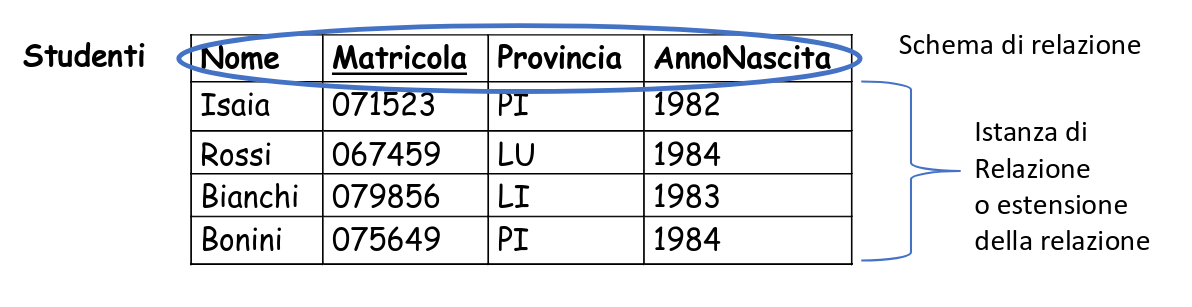
\includegraphics[scale=0.35]{schemarel.png}
\end{center}

\subsection{Valori}
Il modello relazionale è basato su \textbf{valori}, ovvero i riferimenti fra i dati in relazioni diverse sono rappresentati per mezzo di valori dei domini che compaiono nelle ennuple. Questo permette di mantenere \textbf{indipendenza} dalle strutture fisiche, si rappresenta solo i dati necessari e si garantisce \textbf{portabilità}.

\begin{definition}[Valore nullo]
	Il valore nullo denota l'assenza di un valore del dominio.
\end{definition}

\begin{definition}[Valore]
	$t[A]$, per ogni attributo $A$, è un valore nel dominio $dom(A)$ oppure il valore nullo $NULL$.
\end{definition}

\subsection{Vincoli di integrità}
Uno schema relazionale è costituito da un insieme di \textbf{schemi di relazione} e da un insieme di \textbf{vincoli d'integrità} su i possibili valori delle estensioni delle relazioni. Questi ultimi permettono di descrivere più accuratamente la realtà migliorando la \textbf{qualità dei dati} e aiutando nella progettazione

\begin{definition}[Vincolo d'integrità]
	Un vincolo d’integrità è una proprietà che deve essere soddisfatta dalle istanze che rappresentano informazioni corrette per l’applicazione. È espresso mediante una funzione booleana che associa ad ogni istanza il valore vero o falso.
\end{definition}

Esistono due tipi di vincoli: 
\begin{itemize}
	\item \textbf{Intrarelazionali}: devono essere rispettati dai valori contenuti nella relazione considerata. Possono essere sui valori o sulle ennuple.
	\item \textbf{Interrelazionali}: devono essere rispettati da valori contenuti in relazioni diverse
\end{itemize}

\subsubsection{Vincoli di ennupla}
Questi vincoli esprimono condizioni sui valori di ciascuna ennupla, indipendentemente dalle altre. Quando coinvolgono un solo attributo sono chiamati \textbf{vincoli di dominio}.

\newpage
\subsection{Chiave}
Una chiave è un insieme di attributi che identificano le ennuple di una relazione.
\begin{definition}[Chiave]
	Un insieme $K$ di attributi per uno schema di relazione $r$ è:
	\begin{itemize}
		\item \textbf{Superchiave} se $r$ non contiene due ennuple distinte $t_1$ e $t_2$ con $t_1[K]=t_2[K]$
		\item \textbf{Chiave} se è una superchiave \textbf{minimale}, cioè se non contiene un'altra superchiave
	\end{itemize}
\end{definition}
\begin{definition}[Chiave primaria]
	La chiave primaria di uno schema di relazione è una delle chiavi, di solito quella con il minor numero di attributi. Non ammette valori nulli ed è indicata con la sottolineatura.
\end{definition}

\begin{center}
	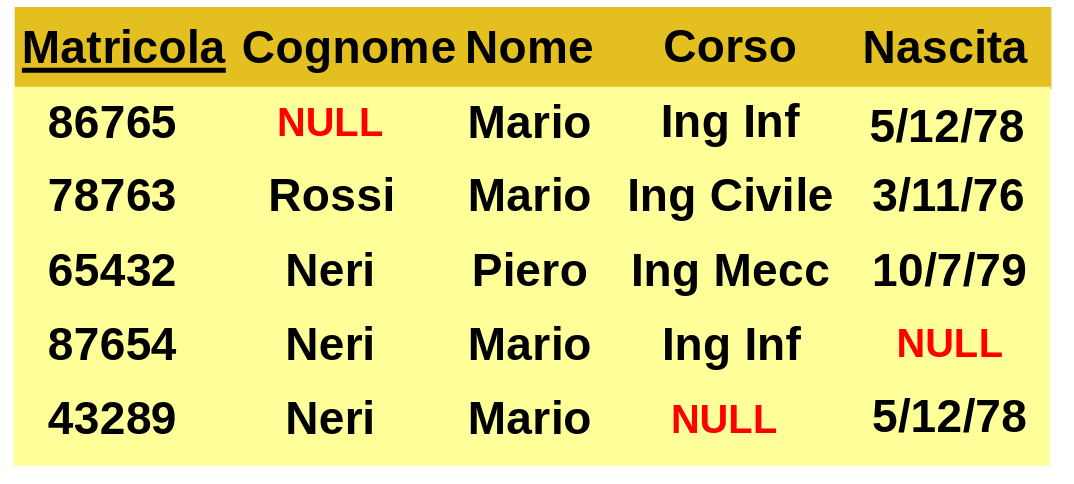
\includegraphics[scale=0.2]{chiave.png}
\end{center}

\begin{note}
	È possibile che esistano degli insiemi di attributi che soddisfino casualmente tutti i vincoli per essere chiavi, ma questo deve succedere \textbf{sempre} per tutte le istanze.
\end{note}

\begin{observation}[Esistenza]
	Ogni relazione ha come superchiave l'insieme di tutti gli attributi su cui è definita, quindi ha sempre almeno una chiave.
\end{observation}

\subsection{Integrità referenziale}
Nel modello relazionale le informazioni in relazioni sono correlate attraverso \textbf{valori} comuni, spesso quelli delle \textbf{chiavi primarie}. Deve quindi esserci una \textbf{coerenza}.\\
Gli attributi che permettono le correlazioni sono indicati sia con la sottolineatura (\textbf{chiavi esterne}) che con l'asterisco.
\begin{center}
	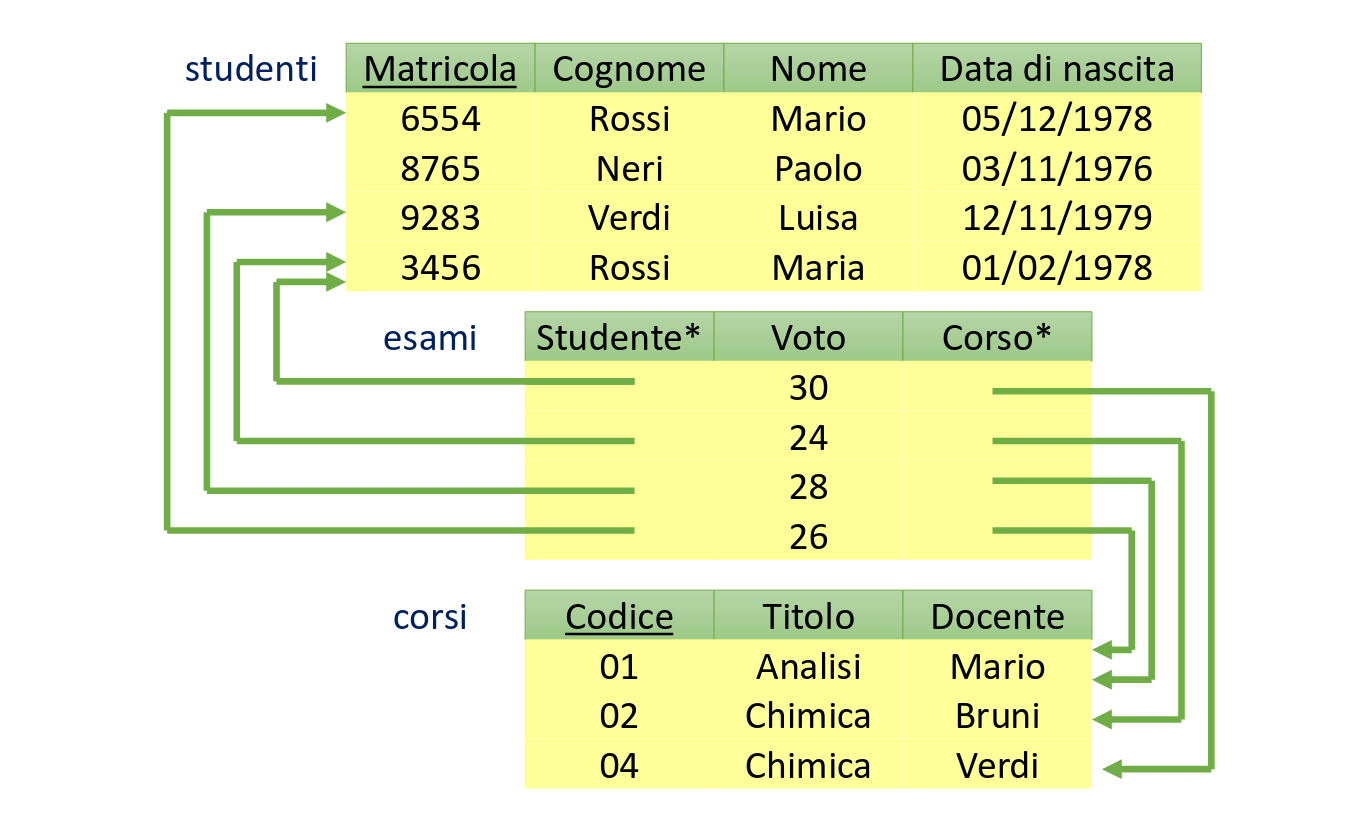
\includegraphics[scale=0.3]{chiaviesterne.png}
\end{center}

\subsubsection{Integrità referenziale}
\begin{definition}[Vincolo di integrità referenziale]
	Un vincolo di integrità referenziale (\textbf{foreign key}) fra gli attributi $X$ di una relazione $R_1$ e un’altra relazione $R_2$ impone ai valori su $X$ in $R_1$ di comparire come valori della chiave primaria di $R_2$.
\end{definition}
In caso di violazione del vincolo di integrità (e.g. viene eliminata una ennupla dalla tabella riferita), è possibile:
\begin{itemize}
	\item Rifiutare l'operazione
	\item Eliminare in cascata nelle altre tabelle
	\item Introdurre valori nulli
\end{itemize}

\begin{note}
	È possibile avere più chiavi esterne e in questo caso ci sono \textbf{vincoli multipli}.
\end{note}
	% !TeX spellcheck = it_IT
\newpage
\section{Trasformazione di schemi}
L'obiettivo della trasformazione è quello di ottenere da uno schema concettuale uno schema \textbf{logico-relazionale} che rappresenti gli stessi dati in maniera \textbf{corretta} ed \textbf{efficiente}, riducendo la ridondanza e facilitandone la comprensione.\\
Questa trasformazione prende in \textbf{ingresso} lo schema relazionale, il carico applicativo e il modello logico e restituisce in \textbf{uscita} uno schema logico e la documentazione.\\
Si compone dei seguenti passi:
\begin{enumerate}
	\item Rappresentazione delle associazioni uno ad uno e uno a molti
	\item Rappresentazione delle associazioni molti a molti o non binarie
	\item Rappresentazione delle gerarchie di inclusione
	\item Identificazione delle chiavi primarie
	\item Rappresentazione degli attributi multivalore
	\item Appiattimento degli attributi composti
\end{enumerate}

\begin{example}[Esempio di trasformazione]
	Dato il seguente schema concettuale
	\begin{center}
		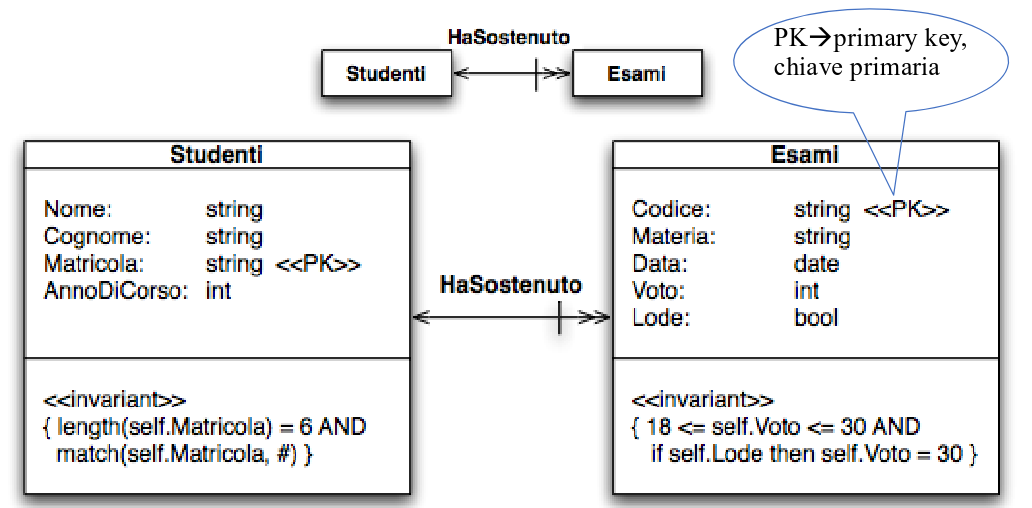
\includegraphics[scale=0.35]{esempiotrasformazione.png}
	\end{center}
	per ottenere uno schema logico introduciamo l'attributo \textbf{matricola}. Questo ci porta ad avere due relazioni collegate dal nuovo attributo.
	\begin{center}
		\begin{tabular}{|c|c|c|c|}
			\hline
			\textbf{Nome} & \textbf{\underline{Matricola}} & \textbf{Provincia} & \textbf{AnnoNascita} \\
			\hline
			Isaia & 071523 & PI & 1982 \\
			\hline
			Rossi & 067459 & LU & 1984 \\
			\hline
			Bianchi & 079856 & LI & 1983 \\
			\hline
			Bonini & 075649 & PI & 1984 \\
			\hline
		\end{tabular}
	\end{center}
	\begin{center}		
		\begin{tabular}{|c|c|c|c|}
			\hline
			\textbf{\underline{Materia}} & \textbf{\underline{Candidato*}} & \textbf{Data} & \textbf{Voto} \\
			\hline
			BD & 071523 & 12/01/06 & 28 \\
			\hline
			BD & 067459 & 15/09/06 & 30\\
			\hline
			FP & 079856 & 25/10/06 & 30 \\
			\hline
			BD & 075649 & 27/06/06 & 25 \\
			\hline
			LMM & 071523 & 10/10/06 & 18 \\
			\hline
		\end{tabular}
	\end{center}
\end{example}
\newpage
\subsection{Rappresentazioni}
\subsubsection{Uno a molti/uno}
\paragraph{Uno a molti}
Le associazioni uno a molti si rappresentano aggiungendo agli attributi della relazione rispetto a cui l’associazione è univoca una \textbf{chiave esterna} che riferisce l’altra relazione. Se l’associazione ha degli attributi, questi si aggiungono alla relazione in cui è presente la chiave esterna.

\begin{center}
	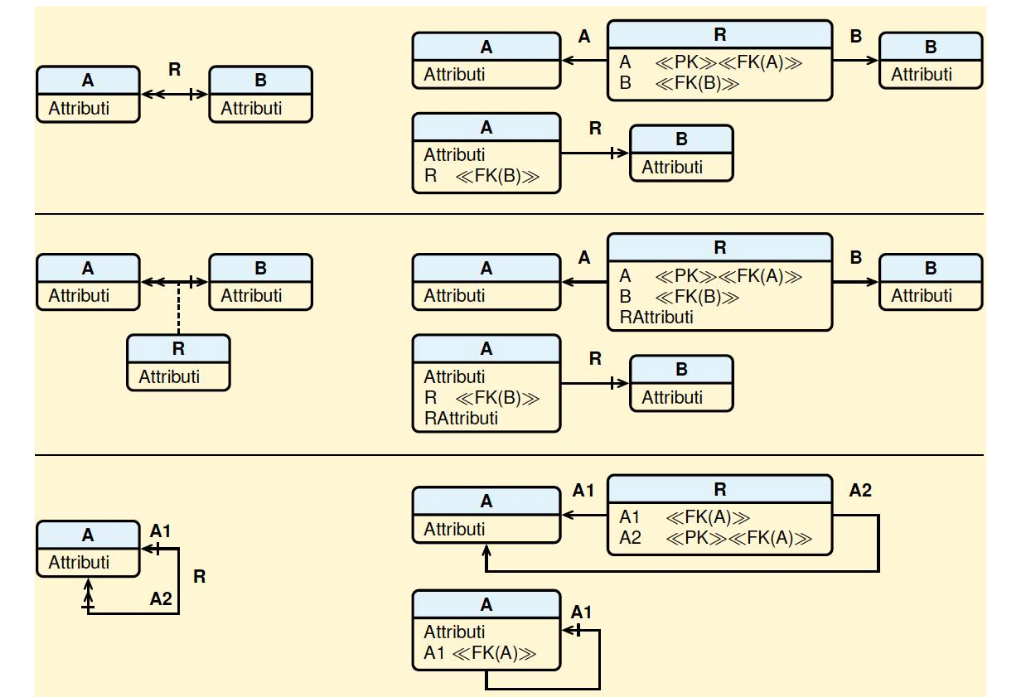
\includegraphics[scale=0.4]{trasfunomolti.png}
\end{center}

\paragraph{Uno ad uno}
Le associazioni uno a uno si rappresentano aggiungendo la \textbf{chiave esterna} ad una qualunque delle due relazioni che riferisce l’altra relazione, preferendo quella rispetto a cui l’associazione è totale, nel caso in cui esista un vincolo di totalità.
\begin{center}
	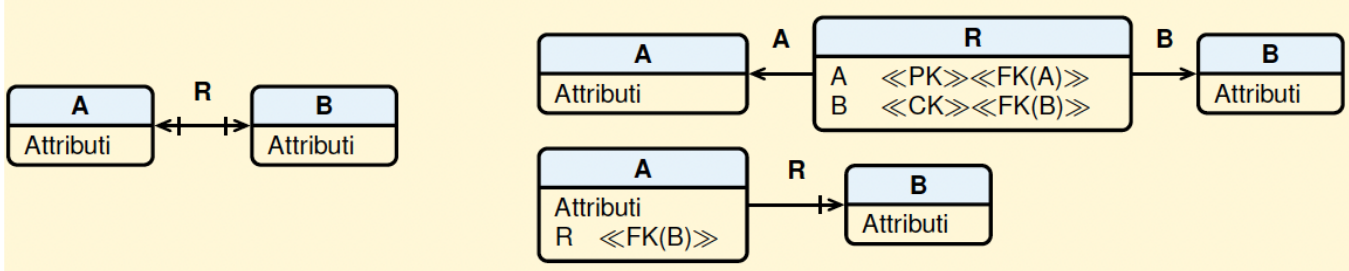
\includegraphics[scale=0.3]{trasfunouno.png}
\end{center}

\paragraph{Vincoli}
\begin{definition}[Diretta]
	La direzione dell’associazione rappresentata dalla chiave esterna è	detta \textbf{la diretta} dell’associazione.
\end{definition}

I vincoli sulla \textbf{cardinalità} delle associazioni \textbf{uno ad uno} e \textbf{uno a molti} sono:
\begin{itemize}
	\item \textbf{Univocità} della diretta
	\item \textbf{Totalità} della diretta: vincolo \textit{not null} sulla chiave esterna
	\item \textbf{Univocità} dell'inversa e \textbf{totalità} della diretta: vincolo \textit{not null} e \textit{di chiave} sulla chiave esterna
\end{itemize}
\subsubsection{Molti a molti}
Un’associazione molti a molti si rappresenta aggiungendo allo schema una nuova relazione che contiene due chiavi esterne che riferiscono le due relazioni coinvolte; la chiave primaria di questa relazione è costituita dall’insieme di tutti i suoi attributi.

\begin{center}
	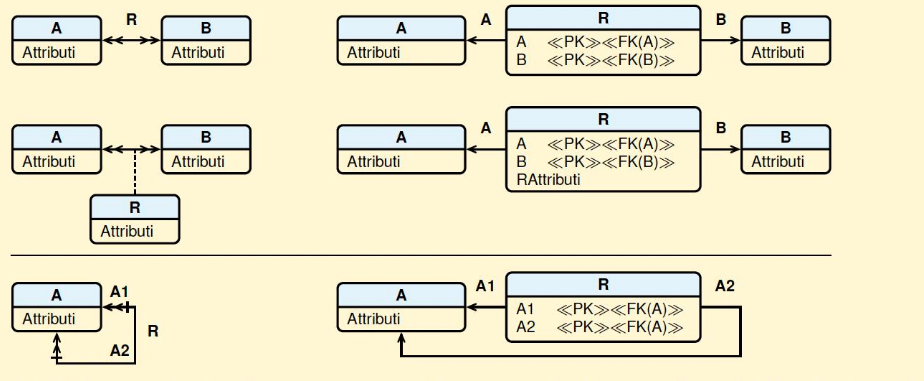
\includegraphics[scale=0.45]{trasfmoltimolti.png}
\end{center}

\subsubsection{Gerarchie tra classi}
Il modello relazionale non può rappresentare le gerarchia tra classi. Bisogna quindi eliminarle e sostituirle con classi e relazioni usando le seguenti tecniche:
\begin{itemize}
	\item \textbf{Relazione unica}: accorpamento delle figlie nel genitore
	\item \textbf{Partizionamento orizzontale}: accorpamento del genitore nelle figlie
	\item \textbf{Partizionamento verticale}: sostituzione della gerarchia con relazioni
\end{itemize}

\paragraph{Relazione unica}
Si seguono i seguenti passi:
\begin{enumerate}
	\item Se $A_0$ è la classe genitore di $A_1$ ed $A_2$, queste ultime vengono eliminate ed accorpate alla prima
	\item Ad $A_0$ viene aggiunto un attributo (\textbf{discriminatore}) che indica da quale delle classi figlie deriva una certa istanza, e gli attributi di $A_1$ ed $A_2$ vengono assorbiti dalla classe genitore, e assumono valore nullo sulle istanze provenienti dall’altra classe
	\item Infine, una relazione relativa a solo una delle classi figlie viene acquisita dalla classe genitore e avrà comunque cardinalità minima uguale a $0$, in quanto gli elementi dell’altra classe non contribuiscono alla relazione.
\end{enumerate}

\begin{center}
	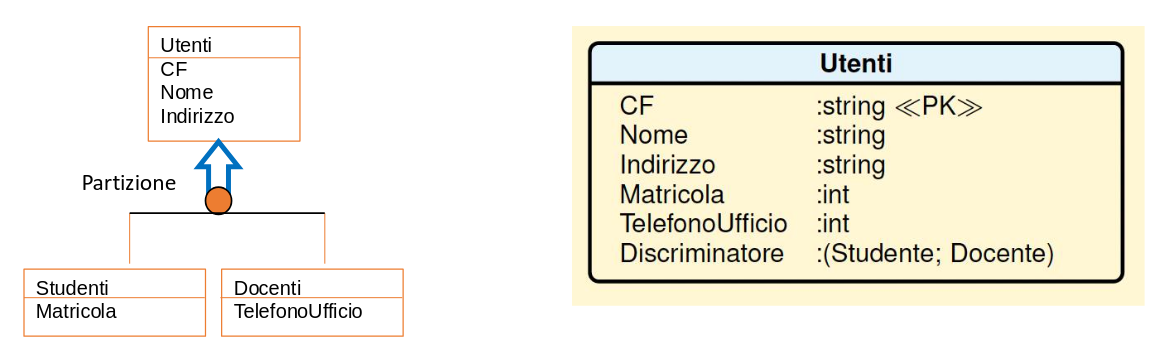
\includegraphics[scale=0.35]{relunica.png}
\end{center}

\newpage
\paragraph{Partizionamento orizzontale}
Se $A_0$ è la classe genitore di $A_1$ ed $A_2$, la classe genitore viene eliminata, e le classi figlie ereditano le proprietà (attributi,identificatore e relazioni) della classe genitore.

\begin{center}
	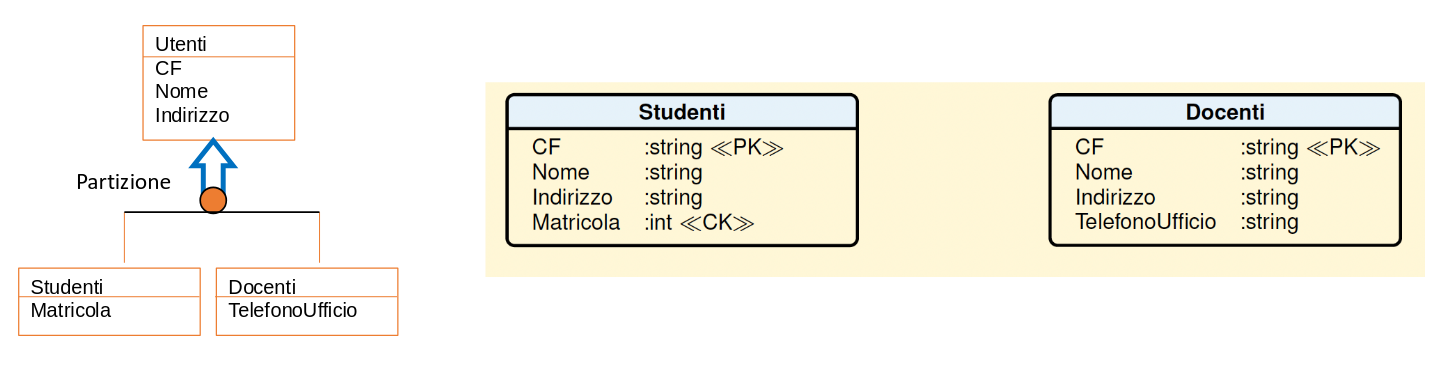
\includegraphics[scale=0.3]{partorizz.png}
\end{center}

\begin{note}
	Questa tecnica divide gli elementi della superclasse $A_0$ in più relazioni diverse, per cui non è possibile mantenere un vincolo referenziale verso $A_0$. In conclusione, questa tecnica non si usa se
	nello schema relazionale c’è una associazione diretta verso $A_0$, ovvero che entra nella superclasse.
\end{note}

\paragraph{Partizionamento verticale}
In questo caso non c’è un trasferimento di attributi o di associazioni e le classi figlie $A_1$ ed $A_2$ sono identificate esternamente dalla classe genitore $A_0$. Nello schema ottenuto vanno aggiunti dei vincoli: ogni occorrenza di $A_0$ non può partecipare contemporaneamente alle due associazioni, e se la gerarchia è totale, deve partecipare ad almeno una delle due.

\begin{center}
	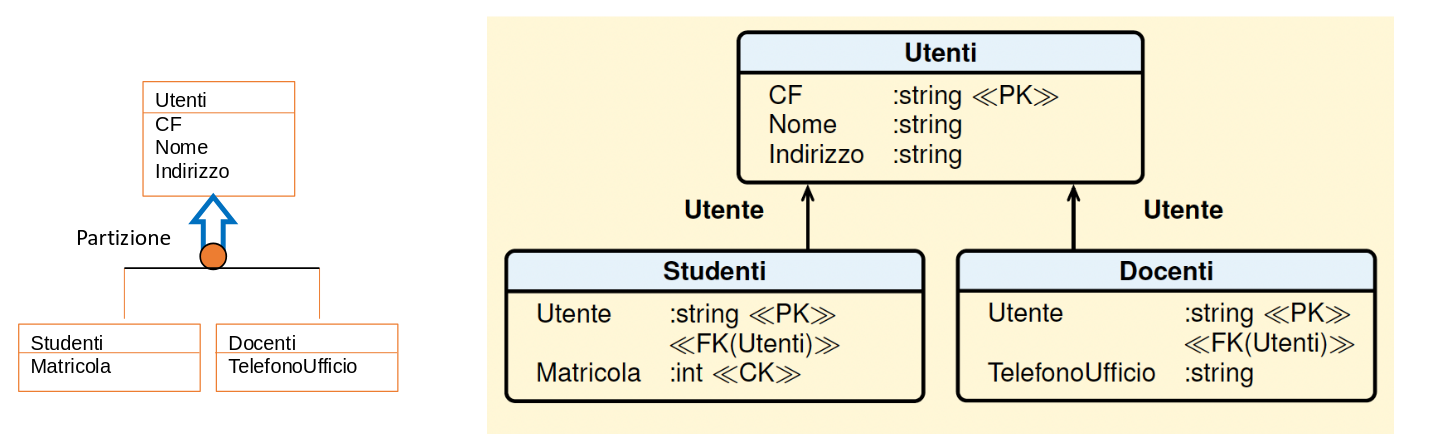
\includegraphics[scale=0.3]{partvert.png}
\end{center}

\subsubsection{Chiavi primarie}
È necessario definire per ogni relazione un insieme di attributi che funga da chiave primaria, seguendo questi passi:
\begin{enumerate}
	\item Si considerano le relazioni che corrispondono a classi dello schema originale	che erano prive di superclassi (\textbf{classi radice}). La chiave primaria è di norma un attributo artificiale, tipicamente un numero progressivo	assegnato dal sistema. E’ possibile utilizzare un attributo presente nella classe, purché
	l’attributo sia \textbf{univoco}, \textbf{totale} e \textbf{costante}.
	\item Per ogni relazione dello schema che corrisponde ad una \textbf{sottoclasse} dello schema originario, la chiave primaria sarà la stessa della superclasse.
	\item Per le relazioni che corrispondono ad $\mathbf{N:M}$ nello schema originario, la chiave primaria sarà costituita dalla concatenazione delle chiavi esterne.
\end{enumerate}

\newpage
\subsubsection{Attributi multivalore}
Una proprietà multivalore di una classe $C$ si rappresenta eliminando il corrispondente attributo da $C$ e creando una nuova relazione $N$ con una chiave di due attributi:
\begin{itemize}
	\item una \textbf{chiave esterna} che fa riferimento alla chiave primaria di $C$
	\item un \textbf{attributo} che corrisponde all’attributo multivalore da trasformare
\end{itemize}
Un oggetto di $C$ con chiave primaria $k$ ed in cui l’attributo assume valore $a_1, \ldots, a_n$ si rappresenta poi inserendo nella relazione $N$ le coppie $(k, a_1), \ldots , (k, a_n)$

\begin{center}
	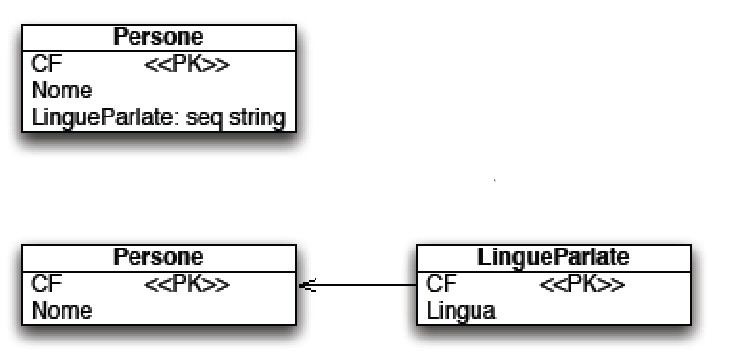
\includegraphics[scale=0.4]{multival.png}
\end{center}

\subsubsection{Attributi composti}
Se un attributo $A_i$ di uno schema di relazione è di tipo $[A_{i1} : T_{i1}, \ldots , A_{ij} :
T_{ij}]$, si sostituisce con gli attributi $A_{i1} : T_{i1}, \ldots, A_{ij} : T_{ij}$. Se $A_i$ faceva parte della chiave primaria dello schema di relazione, si sostituisce $A_i$ con gli attributi $A_{i1}, \ldots, A_{ij}$ nella chiave, e poi si verifica che non esista un sottoinsieme degli attributi della nuova chiave primaria che è esso stesso una chiave.

\begin{example}
	Dato l'attributo composto
	\begin{equation*}
		[\text{Via} : \text{string}, \text{Numero} : \text{int}, \text{Citta}:\text{string}]
	\end{equation*}
	otteniamo
	\begin{center}
		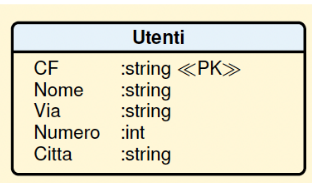
\includegraphics[scale=0.4]{composti.png}
	\end{center}
\end{example}
	% !TeX spellcheck = it_IT
\newpage
\section{Algebra relazionale}
L'\textbf{algebra relazionale} è l'insieme degli operatori su relazioni che danno come risultato relazioni. Viene usato come rappresentazione interna delle interrogazioni e non come linguaggio di interrogazione dei DBMS.\\
Il \textbf{calcolo relazionale} è invece il linguaggio dichiarativo di tipo logico dal quale è stato derivato SQL.

\subsection{Notazione}
\paragraph{Nomi di relazioni} $R, S, \ldots$
\paragraph{Nomi di attributi} $A, B, C, A_1, A_2, \ldots$
\paragraph{Insiemi di attributi} $X, Y, X_1, \ldots$
\paragraph{Unione di insiemi di attributi} $X \cup Y = XY$
\paragraph{Relazione con ennuple} Date le ennuple $t_1, t_2, \ldots, t_n$ la relazione è denotata con $\{t_1, t_2, \ldots, t_n\}$
\paragraph{Relazione vuota} $\{\}$
\paragraph{Valore attributo} Data la ennupla $t_k$, il suo valore $A_i$ è denotato da $t_k.A_i$
\paragraph{Ennupla specifica ad attributi} Se $X$ è sottoinsieme degli attributi di $t$, $t.X$ o $t[X]$ allora denota l’ennupla ottenuta da $t$ considerando solo gli attributi in $X$
\paragraph{Ambiguità} Se $R$ ed $S$ hanno lo stesso attributo $A_j$, in caso di ambiguità, $R.A_j$ denota l’attributo $A_j$ della relazione $R$ ed $S.A_j$ denota l’attributo $A_j$ della relazione $S$.

\newpage
\subsection{Operatori primitivi}
\subsubsection{Ridenominazione}
Viene utilizzato per cambiare il nome di una relazione e di conseguenza anche il suo \textbf{tipo}.
\begin{equation}
	\rho_{A \leftarrow B}(R)
\end{equation}
\begin{equation}
	T' = \rho_{A \leftarrow A'}(T)
\end{equation}
\begin{table}[!h]
	\centering
	\begin{tabular}{|c|c|c|}
		\hline
		\textbf{Id} & \textbf{Nome} & \textbf{Età} \\
		\hline
		7274 & Rossi & 42 \\
		\hline
		7432 & Neri & 54 \\
		\hline
		9824 & Verdi & 45 \\
		\hline
	\end{tabular}
	\hspace{10pt} $\longrightarrow$ \hspace{10pt}
	\begin{tabular}{|c|c|c|}
		\hline
		\textbf{Matricola} & \textbf{Nome} & \textbf{Età} \\
		\hline
		7274 & Rossi & 42 \\
		\hline
		7432 & Neri & 54 \\
		\hline
		9824 & Verdi & 45 \\
		\hline
	\end{tabular}
	\caption{Laureati}
\end{table}

\subsubsection{Unione}
Restituisce la relazione ottenuta facendo l’unione delle ennuple di $R$ con quelle di $S$ dove $R$ e $S$ sono relazioni dello stesso tipo.

\begin{equation}
	R \cup S
\end{equation}

\begin{table}[!h]
	\centering
	\begin{tabular}{|c|c|c|}
		\hline
		\textbf{\underline{A}} & \textbf{\underline{B}} & \textbf{\underline{C}} \\
		\hline
		a1 & b1 & c1 \\
		\hline
		a1 & b1 & c2 \\
		\hline
		a2 & b1 & c1 \\
		\hline
		a3 & b1 & c1 \\
		\hline
	\end{tabular}
	\hspace{10pt} $\cup$ \hspace{10pt}
	\begin{tabular}{|c|c|c|}
		\hline
		\textbf{\underline{A}} & \textbf{\underline{B}} & \textbf{\underline{C}} \\
		\hline
		a1 & b1 & c1 \\
		\hline
		a1 & b2 & c2 \\
		\hline
	\end{tabular}
	\hspace{10pt} $\longrightarrow$ \hspace{10pt}
	\begin{tabular}{|c|c|c|}
		\hline
		\textbf{A} & \textbf{B} & \textbf{C} \\
		\hline
		a1 & b1 & c1 \\
		\hline
		a1 & b1 & c2 \\
		\hline
		a1 & b2 & c2 \\
		\hline
		a2 & b1 & c1 \\
		\hline
		a3 & b1 & c1 \\
		\hline
	\end{tabular}
\end{table}
\subsubsection{Differenza}
Restituisce la relazione contenente le ennuple di $R$ non presenti in $S$.

\begin{equation}
	R-S
\end{equation}

\begin{table}[!h]
	\centering
	\begin{tabular}{|c|c|c|}
		\hline
		\textbf{\underline{A}} & \textbf{\underline{B}} & \textbf{\underline{C}} \\
		\hline
		a1 & b1 & c1 \\
		\hline
		a1 & b1 & c2 \\
		\hline
		a2 & b1 & c1 \\
		\hline
		a3 & b1 & c1 \\
		\hline
	\end{tabular}
	\hspace{10pt} $-$ \hspace{10pt}
	\begin{tabular}{|c|c|c|}
		\hline
		\textbf{\underline{A}} & \textbf{\underline{B}} & \textbf{\underline{C}} \\
		\hline
		a1 & b1 & c1 \\
		\hline
		a1 & b2 & c2 \\
		\hline
	\end{tabular}
	\hspace{10pt} $\longrightarrow$ \hspace{10pt}
	\begin{tabular}{|c|c|c|}
		\hline
		\textbf{A} & \textbf{B} & \textbf{C} \\
		\hline
		a1 & b1 & c2 \\
		\hline
		a2 & b1 & c1 \\
		\hline
		a3 & b1 & c1 \\
		\hline
	\end{tabular}
\end{table}

\newpage
\subsubsection{Proiezione}
Restituisce una relazione i cui elementi sono la copia delle ennuple di $R$ proiettate (ristrette) sugli attributi $A_1,\ldots, A_n$. Eventuali ennuple che dopo la proiezione sono uguali appaiono solo una volta.
\begin{equation}
	\pi_{A_1, \ldots, A_n} (R)
\end{equation}
Data la tabella usata negli esempi precedenti, la proiezione è:
\begin{table}[!h]
	\centering
	$\pi_A(R)=$ \hspace{10pt}
	\begin{tabular}{|c|}
		\hline
		\textbf{A} \\ 
		\hline
		a1 \\
		\hline
		a2 \\
		\hline
		a3\\
		\hline
	\end{tabular}
\end{table}
\paragraph{Cardinalità}
Una proiezione conterrà al più tante ennuple quanto l'operando:
\begin{itemize}
	\item  Se $X$ è una \textbf{superchiave} di $R$, allora $\pi_X(R)$ contiene esattamente tante ennuple quante $R$
	\item \textbf{Altrimenti} potrebbero esistere valori ripetuti su quegli attributi, che quindi vengono rappresentati una sola volta
\end{itemize}

\subsubsection{Restrizione o selezione}
Restituisce una relazione dello stesso tipo (schema) di $R$ i cui elementi sono la copia delle ennuple di $R$ (un sottoinsieme) che soddisfano la condizione $\phi$ definita come:
\begin{itemize}
	\item $A_i \phi A_j$ con $A_i$ e $A_j$ attributi di $R$ e $\theta$ un operatore di confronto $\{<, >, =, \neq, \leq, \geq \}$
	\item $A_i \theta c$ oppure $c \theta A_i$, con $\theta$ operatore di confronto e $c$ costante nel dominio di $A_i$
	\item Se $\phi$ e $\psi$ sono formule, allora lo sono anche $\phi \land \psi$, $\phi \lor \psi$ e $\neg \psi$
\end{itemize}
\begin{equation}
	\sigma_\phi(R)
\end{equation}
Data la tabella usata negli esempi precedenti abbiamo
\begin{table}[!h]
	\centering
	$\sigma_{A=a_1}(R)=$ \hspace{10pt}
	\begin{tabular}{|c|c|c|}
		\hline
		\textbf{A} & \textbf{B} & \textbf{C}\\ 
		\hline
		a1 & b1 & c1\\
		\hline
		a1 & b1 & c2\\
		\hline
	\end{tabular}
\end{table}

\begin{observation}[Valori nulli]
	La presenza di valori \textbf{nulli} negli attributi usati per la restrizione portano all'assenza di \textbf{atomicità} nell'operazione.
	\begin{equation*}
		\sigma_{\text{Età}>30}(\text{Persone}) \cup \sigma_{\text{Età}\leq30}(\text{Persone}) \neq \text{Persone}
	\end{equation*}
	Per mantenerla è quindi necessario utilizzare i costrutti \textit{IS NULL} e \textit{IS NOT NULL}:
	\begin{equation*}
		\sigma_{\text{Età}>30}(\text{Persone}) \cup \sigma_{\text{Età}\leq30}(\text{Persone}) \cup \sigma_{\text{Età IS NULL}}(\text{Persone}) = \text{Persone}
	\end{equation*}
\end{observation}

\newpage
\subsubsection{Prodotto}
Con $R$ e $S$ relazioni con attributi distinti, il loro prodotto è una relazione con elementi ottenuti concatenando ogni ennupla di $R$ con ogni ennupla di $S$. La relazione risultante ha grado uguale alla somma dei gradi degli operandi e cardinalità uguale al prodotto delle cardinalità degli operandi.
\begin{equation}
	R \times S
\end{equation}
\begin{table}[!h]
	\centering
	\begin{tabular}{|c|c|c|}
		\hline
		\textbf{\underline{A}} & \textbf{\underline{B}} & \textbf{\underline{C}} \\
		\hline
		a1 & b1 & c1 \\
		\hline
		a1 & b1 & c2 \\
		\hline
		a2 & b1 & c1 \\
		\hline
		a3 & b1 & c1 \\
		\hline
	\end{tabular}
	\hspace{10pt} $\times$ \hspace{10pt}
	\begin{tabular}{|c|c|}
		\hline
		\textbf{A'} & \textbf{D} \\
		\hline
		a1 & d1 \\
		\hline
		a2 & d2 \\
		\hline
	\end{tabular}
	\hspace{10pt} $\longrightarrow$ \hspace{10pt}
	\begin{tabular}{|c|c|c|c|c|}
		\hline
		\textbf{A} & \textbf{B} & \textbf{C} & \textbf{A'} & \textbf{D} \\
		\hline
		a1 & b1 & c1 & a1 & d1 \\
		\hline
		a1 & b1 & c1 & a2& d2 \\
		\hline
		a1 & b1 & c2 & a1 & d1 \\
		\hline
		a1 & b1 & c2 & a2 & d2 \\
		\hline
		a2& b1 & c1 & a1 & d1 \\
		\hline
		a2 & b1 & c1 & a2 & d2 \\
		\hline
		a3 & b1 & c1 & a1 & d1 \\
		\hline
		a3 & b1 & c1 & a2 & d2 \\
		\hline		
	\end{tabular}
\end{table}

\begin{observation}
	Il prodotto di due relazioni è un’operazione che di solito non si usa da sola. Pertanto per concatenare ennuple in associazione, si restringe sempre il prodotto alle ennuple con valore uguale della chiave esterna e chiave primaria. Per questa si introduce un operatore derivato, chiamato \textbf{giunzione}, per riferirsi alla combinazione di queste due operazioni.
\end{observation}

\subsection{Operatori derivati}
\subsubsection{Intersezione}
Restituisce la relazione ottenuta facendo l’intersezione delle ennuple di $R$ con quelle di $S$ dove $R$ e $S$ sono relazioni dello stesso tipo.

\begin{equation}
	R \cap S = R - (R-S)
\end{equation}

\begin{table}[!h]
	\centering
	\begin{tabular}{|c|c|c|}
		\hline
		\textbf{\underline{A}} & \textbf{\underline{B}} & \textbf{\underline{C}} \\
		\hline
		a1 & b1 & c1 \\
		\hline
		a1 & b1 & c2 \\
		\hline
		a2 & b1 & c1 \\
		\hline
		a3 & b1 & c1 \\
		\hline
	\end{tabular}
	\hspace{10pt} $\cap$ \hspace{10pt}
	\begin{tabular}{|c|c|c|}
		\hline
		\textbf{\underline{A}} & \textbf{\underline{B}} & \textbf{\underline{C}} \\
		\hline
		a1 & b1 & c1 \\
		\hline
		a1 & b2 & c2 \\
		\hline
	\end{tabular}
	\hspace{10pt} $\longrightarrow$ \hspace{10pt}
	\begin{tabular}{|c|c|c|}
		\hline
		\textbf{A} & \textbf{B} & \textbf{C} \\
		\hline
		a1 & b1 & c1 \\
		\hline
	\end{tabular}
\end{table}

\subsubsection{Inner Join}
Restituisce la relazione contenente le ennuple del prodotto cartesiano di $R \times S$ con valori uguali per gli attributi $A_i$ e $A_j$ dove $R$ e $S$ sono relazioni di tipo diverso (con attributi distinti) tra i quali c’è $A_i$ in $R$ e $A_j$ in $S$.
\begin{equation}
	R \Join_{A_i = A_j}S = \sigma_{A_i=A_j}(R \times S)
\end{equation}
Date le tabelle usate come esempio nel prodotto ($R$ e $T'$), abbiamo
\begin{table}[!h]
	\centering
	$R \Join_{A=A'}T' =$ \hspace{10pt}
	\begin{tabular}{|c|c|c|c|c|}
		\hline
		A & B & C & A' & D \\
		\hline
		a1 & b1 & c1 & a1 & d1 \\
		\hline
		a1 & b1 & c2& a1 & d1 \\
		\hline
		a2 & b1 & c1 & a2 & d2 \\
		\hline
	\end{tabular}
\end{table}

\subsubsection{Theta Join}
È il caso più generale della \textit{Inner Join}: qui la condizione $\theta$ è una congiunzione di termini logici di confronto ($>$, $<$, $=$, $\ldots$).
\begin{equation}
	R \Join_\sigma S
\end{equation}

\subsubsection{Natural Join}
È una abbreviazione dell’\textit{Inner Join} applicata a relazioni in cui l’associazione fra le ennuple è
descritta con la chiave esterna e la chiave primaria costituite da attributi uguali. Restituisce la relazione contenente le ennuple di $R \times S$ con gli attributi di uguali nomi in $R$ ed $S$ definiti sugli stessi domini. 
\begin{equation}
	R \Join S = R \Join_{A=A}S = \sigma_{A=A}(R \times S)
\end{equation}

\begin{table}[!h]
	\centering
	\begin{tabular}{|c|c|c|}
		\hline
		\textbf{\underline{A}} & \textbf{\underline{B}} & \textbf{\underline{C}} \\
		\hline
		a1 & b1 & c1 \\
		\hline
		a1 & b1 & c2 \\
		\hline
		a2 & b1 & c1 \\
		\hline
		a3 & b1 & c1 \\
		\hline
	\end{tabular}
	\hspace{10pt} $\Join$ \hspace{10pt}
	\begin{tabular}{|c|c|}
		\hline
		\textbf{\underline{A}} & \textbf{D} \\
		\hline
		a1 & d1 \\
		\hline
		a2 & d2 \\
		\hline
	\end{tabular}
	\hspace{10pt} $\longrightarrow$ \hspace{10pt}
	\begin{tabular}{|c|c|c|c|}
		\hline
		\textbf{A} & \textbf{B} & \textbf{C} & \textbf{D} \\
		\hline
		a1 & b1 & c1 & d1\\
		\hline
		a1 & b1 & c2 & d1 \\
		\hline
		a2 & b1 & c1 & d2 \\
		\hline
	\end{tabular}
\end{table}

\begin{note}
	Si noti che:
	\begin{itemize}
		\item Se $R$ ed $S$ non hanno attributi comuni allora $R \Join S = R \times S$
		\item Se $R$ ed $S$ hanno lo stesso schema allora $R \Join S = R \cap S$
	\end{itemize}
\end{note}

\paragraph{Cardinalità} Date le relazioni $R_1(A,B)$ e $R_2(B, C)$:
\begin{itemize}
	\item Il numero di ennuple della loro join è:
	\begin{equation*}
		0 \leq \lvert R_1 \Join R_2 \rvert \leq \lvert R_1 \rvert \times \lvert R_2 \rvert
	\end{equation*}
	\item Se il loro join è \textbf{completo} allora contiene un numero di ennuple almeno uguale al massimo tra $\lvert R_1 \rvert$ e $\lvert R_2 \rvert$
	\item Se il join coinvolge una \textbf{chiave} $B$ di $R_2$ allora:
	\begin{equation*}
		0 \leq \lvert R_1 \Join R_2 \rvert \leq \lvert R_1 \rvert 
	\end{equation*}
	\item Se il join coinvolge una \textbf{chiave} $B$ di $R_2$ e un \textbf{vincolo di integrità referenziale} tra gli attributi di $R_1$ e la chiave di $R_2$ allora:
	\begin{equation*}
		\lvert R_1 \Join R_2 \rvert = \lvert R_1 \rvert
	\end{equation*}
\end{itemize}

\begin{observation}[Natural Join e Proiezione]
	Osserviamo che valgono due cose:
	\begin{itemize}
		\item Dati $R_1(X_1)$ e $R_2(X_2)$ vale
		\begin{equation}
			\pi_{X_1}(R_1 \Join R_2) \subseteq R_1
		\end{equation}
		\item Dati $R(X)$ con $X = X_1 \cup X_2$ vale
		\begin{equation}
			R \subseteq (\pi_{X_1}(R)) \Join (\pi_{X_2}(R))
		\end{equation}
	\end{itemize}
\end{observation}

\newpage
\subsubsection{Semi Join}
Restituisce le ennuple di $R$ che partecipano alla giunzione naturale di $R$ ed $S$ con $A_1, A_2, \ldots, A_m$ attributi di $R$.
\begin{equation}
	R S = \pi_{A_1, A_2, \ldots, A_m}(R \Join S)
\end{equation}
Considerando l'esempio precedente abbiamo
\begin{table}[!h]
	\centering
	$R T =$\hspace{10pt}
	\begin{tabular}{|c|c|c|}
		\hline
		\textbf{A} & \textbf{B} & \textbf{C} \\
		\hline
		a1 & b1 & c1 \\
		\hline
		a1 & b1 & c2 \\
		\hline
		a2 & b1 & c1 \\
		\hline
	\end{tabular}
\end{table}

\subsubsection{External Join}
Il join esterno estende con valori nulli le ennuple che verrebbero tagliate fuori da un join interno. Ne esistono tre versioni:
\begin{itemize}
	\item \textbf{Left}: mantiene tutte le ennuple del primo operando, estendendole con valori nulli se necessario
	\begin{equation}
		R \overset{\leftarrow}{\Join}S
	\end{equation}
	\item \textbf{Right}: come left ma con il secondo operando
	\begin{equation}
		R \overset{\rightarrow}{\Join} S
	\end{equation}
	\item \textbf{Full}: come left ma con entrambi gli operandi
	\begin{equation}
		R \overset{\leftrightarrow}{\Join} S
	\end{equation}
\end{itemize}

\subsubsection{Self Join}
Questa operazione è utilizzata quando va fatta una join di una tabella con se stessa. Spesso è importante fare anche delle ridenominazioni.

\begin{example}[Nonno nipote]
	Data la relazione
	\begin{table}[!h]
		\centering
		\begin{tabular}{|c|c|}
			\hline
			\textbf{Genitore} & \textbf{Figlio} \\
			\hline
			Luca & Anna \\
			\hline
			Maria & Anna \\
			\hline
			Giorgio & Luca\\
			\hline
			Silvia & Maria \\
			\hline
			Enzo & Maria\\
			\hline
		\end{tabular}
	\end{table}
	effettuiamo le seguenti operazioni
	\begin{equation*}
		\rho_{\text{Genitore}, \text{Figlio} \leftarrow \text{Nonno}, \text{Genitore}}(\text{Genitore}) \Join \rho_{\text{Figlio} \leftarrow \text{Nipote}}(\text{Genitore})
	\end{equation*}
	\begin{table}[!h]
		\centering
		\begin{tabular}{|c|c|}
			\hline
			\textbf{Nonno} & \textbf{Genitore} \\
			\hline
			Luca & Anna \\
			\hline
			Maria & Anna \\
			\hline
			Giorgio & Luca\\
			\hline
			Silvia & Maria \\
			\hline
			Enzo & Maria\\
			\hline
		\end{tabular}
		\hspace{10pt} $\Join$ \hspace{10pt}
		\begin{tabular}{|c|c|}
			\hline
			\textbf{Genitore} & \textbf{Nipote} \\
			\hline
			Luca & Anna \\
			\hline
			Maria & Anna \\
			\hline
			Giorgio & Luca\\
			\hline
			Silvia & Maria \\
			\hline
			Enzo & Maria\\
			\hline
		\end{tabular}
		\hspace{10pt} $=$ \hspace{10pt}
		\begin{tabular}{|c|c|c|}
			\hline
			\textbf{Nonno} & \textbf{Genitore} & \textbf{Nipote} \\
			\hline
			Giorgio & Luca & Anna \\
			\hline
			Silvia & Maria & Anna \\
			\hline
			Enzo & Maria & Anna \\
			\hline
		\end{tabular}
	\end{table}
\end{example}

\subsection{Proprietà algebriche degli operatori}
Un'espressione algebrica può essere rappresentata come un \textbf{albero}:
\[
\begin{aligned}
	& \pi_{\text{Nome}, \text{Matricola}} (\\
	& \qquad \pi_{\text{Nome}, \text{Matricola}}(\sigma_{\text{Provincia} = \text{'PI'}}(\text{Studenti}))\\
	& \qquad \Join_{\text{Matricola} = \text{Candidato}} \\
	& \qquad \pi_{\text{Candidato}} (\sigma_{\text{Voto}=25}(\text{Esami})) \\
	&)
\end{aligned}
\qquad
\raisebox{-20mm}{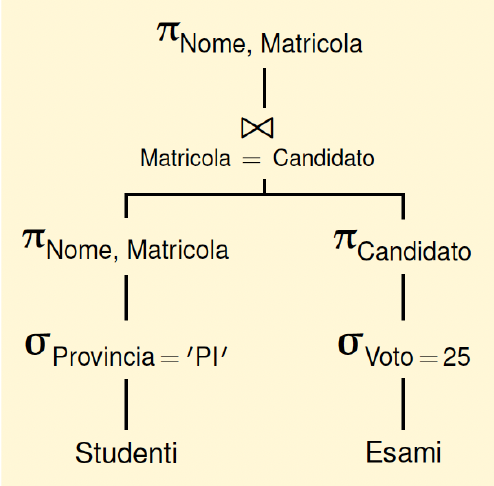
\includegraphics[scale=0.25]{albero.png}}
\]
Un’espressione dell’algebra relazionale può essere trasformata in un’altra equivalente sfruttando alcune proprietà degli operatori. Questo aiuta a ridurre il costo di esecuzione. Le proprietà più utili sono quelle che permettono di anticipare la \textbf{restrizione} e la \textbf{proiezione}:
\begin{itemize}
	\item \textbf{Raggruppamento} di \textbf{restrizioni}
	\begin{equation*}
		\sigma_{C_1}(\sigma_{C_2}(R)) \equiv \sigma_{C_1 \land C_2}(R)
	\end{equation*}
	\item \textbf{Raggruppamento} di \textbf{proiezioni}
	\begin{equation*}
		\sigma_{C_1 \land C_2}(R \times S) \equiv\sigma_{C_1}(R) \times \sigma_{C_2}(S)
	\end{equation*}
	\item \textbf{Commutatività} della \textbf{restrizione}, \textbf{proiezione}, \textbf{prodotto}, \textbf{giunzione} e degli \textbf{operatori insiemistici}
	\begin{equation*}
		(R \times S) \equiv(S \times R)
	\end{equation*}
	\item \textbf{Anticipazione} della \textbf{restrizione} rispetto al prodotto e alla giunzione e rispetto agli operatori insiemistici
	\item \textbf{Anticipazione} della \textbf{proiezione} rispetto al prodotto e alla giunzione e rispetto agli operatori insiemistici
	\item Eliminazioni di proiezioni superflue
	\begin{equation*}
		\pi_{A}(\pi_{A,B}(R)) \equiv \pi_{A}(R)
	\end{equation*}
\end{itemize}

\begin{observation}[Non distributività della proiezione rispetto alla differenza]
	In generale vale che
	\begin{equation}
		\pi_A(R_1 - R_2) \neq \pi_A (R_1)-\pi_A(R_2)
	\end{equation}
\end{observation}

\newpage
\subsection{Quantificatori}
Esistono tre tipi di quantificatori:
\begin{itemize}
	\item \textbf{Esistenziale}: e.g. tutti gli studenti che hanno preso \textit{almeno} un voto maggiore di $28$
	\item \textbf{Differenza}: e.g. tutti gli studenti che NON hanno mai preso un voto maggiore di $28$
	\item \textbf{Universale}: e.g tutti gli studenti che hanno preso SOLO voti maggiori di $28$
\end{itemize}
\begin{figure}[!h]
	\centering
	\begin{minipage}{.3\textwidth}
		\centering
		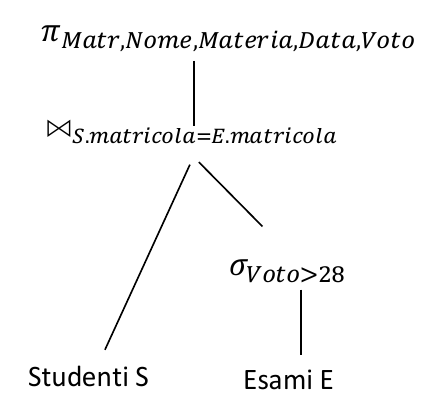
\includegraphics[scale=0.25]{esistenziale.png}
		\captionof{figure}{Esistenziale}
	\end{minipage}
	\begin{minipage}{.3\textwidth}
		\centering
		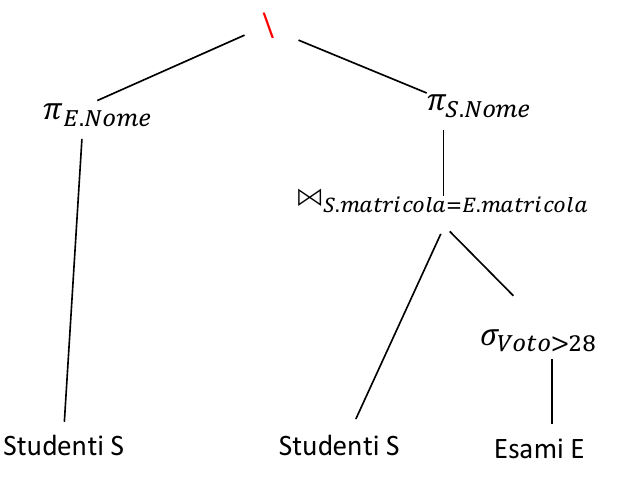
\includegraphics[scale=0.2]{differenza.png}
		\captionof{figure}{Differenza}
	\end{minipage}
	\begin{minipage}{.3\textwidth}
	\centering
	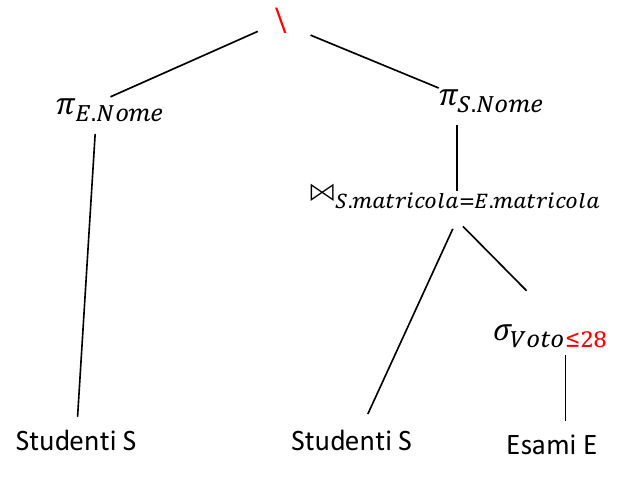
\includegraphics[scale=0.2]{universale.png}
	\captionof{figure}{Universale}
	\end{minipage}
\end{figure}

\subsection{Operatori non insiemistici}
\subsubsection{Group By}
Data una relazione $R$, i suoi attributi $A_i$ e le espressioni che usano funzioni di aggregazione $f_i$ (min, max, count, sum, $\ldots$), definiamo il raggruppamento come una relazione calcolata:
\begin{enumerate}
	\item  Partizionando le ennuple di $R$ mettendo nello stesso gruppo tutte le ennuple con valori uguali degli $A_i$
	\item Si calcolano le espressioni $f_i$ per ogni gruppo
	\item Per ogni gruppo si restituisce una sola ennupla con come attributi i valori degli $A_i$ e delle espressioni $f_i$
\end{enumerate}	
\begin{equation}
	\prescript{}{\{A_i\}\gamma\{f_i\}}{(R)}
\end{equation}
Il raggruppamento gode dell'\textbf{anticipazione} rispetto alla proiezione:
\begin{equation}
	\sigma_C(\prescript{}{X\gamma F}{(R)}) \equiv \prescript{}{X\gamma F}{(\sigma_C(R))}
\end{equation}
\begin{example}
	Vogliamo ottenere per ogni candidato il numero degli esami, il voto minimo, massimo e medio:
	\begin{equation*}
		\prescript{}{\{\text{Candidato}\} \gamma \{\text{count}(*), \min(\text{Voto}), \max(\text{Voto}), \text{avg}(\text{Voto})\}}{(\text{Esami})}
	\end{equation*}
	\begin{table}[!h]
		\centering
		\begin{tabular}{|c|c|c|c|}
			\hline
			\textbf{Materia} & \textbf{Candidato} & \textbf{Voto} & \textbf{Docente} \\
			\hline
			DA & $1$ & $20$ & $10$ \\
			\hline
			LFC & $2$ & $30$ & $20$ \\
			\hline
			MTI & $1$ & $30$ & $30$ \\
			\hline
			LP & $2$ & $20$ & $40$ \\
			\hline
		\end{tabular}\\
		\vspace{10pt} $\downarrow$ \vspace{10pt}\\	
		\begin{tabular}{|c|c|c|c|c|}
			\hline
			\textbf{Candidato} & \textbf{Count(*)} & \textbf{min(Voto)} & \textbf{max(Voto)} & \textbf{avg(Voto)} \\
			\hline
			1 & 2 & 20 & 24 & 22 \\
			\hline
			2 & 2 & 20 & 30 & 25 \\
			\hline
		\end{tabular}
	\end{table}
\end{example}
\subsubsection{Proiezione generalizzata}
Estende la proiezione con la possibilità di usare costanti o espressioni aritmetiche nella lista degli attributi. Permette anche di aggiungere \textbf{etichette} alle espressioni tramite l'operatore \textbf{AS}:
\begin{equation}
	\pi_{e_1\text{ AS } \text{ide}_1, e_2\text{ AS } \text{ide}_2, \ldots}(R)
\end{equation}
Dove $e_1, e_2, \ldots$ sono espressioni aritmetiche ottenute a partire da costanti e $\text{ide}_1, \text{ide}_2, \ldots$ sono etichette distinte.
\subsubsection{Proiezione multi-insiemistica}
Funziona come la proiezione ma senza eliminazione dei duplicati. Restituisce dei multi-insiemi e quindi si possono utilizzare solo come radice di un albero logico.
\begin{equation}
	\pi^b_{\{A_i\}}(R)
\end{equation}
\subsubsection{Ordinamento}
Ordina tutte le ennuple di $R$ in ordine crescente o decrescente rispetto agli attributi $A_i$.
\begin{equation}
	\tau_{\{A_i\}}(R)
\end{equation}

\subsection{Calcolo relazionale}
Il calcolo relazionale è un linguaggio che permette di definire il risultato di un’interrogazione (\textbf{query}) come l’insieme di quelle ennuple che soddisfano una certa condizione $\phi$.\\

L’algebra dà la possibilità di scrivere espressioni in cui gli operatori sono applicati al risultato di altri operatori (espressioni annidate). Il calcolo ha una \textbf{struttura piatta} ma permette di esprimere condizioni più \textbf{complesse}.\\
Un linguaggio che si colloca a metà tra i due stili si può ottenere:
\begin{enumerate}
	\item Aggiungendo al calcolo la possibilità di annidare il costruttore di insiemi
	\item Aggiungendo all’algebra la possibilità di avere nell’operatore di restrizione	condizioni che fanno uso anche di quantificatori e di predicati di appartenenza.
\end{enumerate}
Il risultato è un linguaggio che ha sia la capacità di esprimere interrogazioni in modo annidato che la possibilità di esprimere condizioni logiche complesse, come accade nel linguaggio SQL.

\begin{example}
	L’insieme delle matricole degli Studenti che hanno superato qualcuno degli esami elencati nella relazione Materie, si può definire come
	\begin{align*}
		& \{t.\text{Matricola} \vert t \in \text{Studenti}, \exists m \in \text{Materie}. \exists e \in \text{ProveEsami}.\\
		& e.\text{Candidato}=t.\text{Matricola} \land e.\text{Materia} = m.\text{Materia}\}
	\end{align*}
	che equivale a
	\begin{equation*}
		\pi_{\text{Matricola}}(\text{Studenti} \underset{\text{Matricola} = \text{Candidato}}{\Join}(\text{ProveEsami} \Join \text{Materie}))
	\end{equation*}
\end{example}
	% !TeX spellcheck = it_IT
\newpage
\section{Data Definition Language}
\subsection{Viste}
Le \textbf{Viste Logiche} possono essere definite come delle tabelle \textbf{virtuali}, i cui dati sono riaggregazioni dei dati contenuti nelle tabelle fisiche, senza contenerli effettivamente.\\
Le viste permettono di \textbf{semplificare} la rappresentazione dei dati ed evitare di ripetere query molto complesse. Forniscono inoltre un'ulteriore \textbf{sicurezza} in quanto si può fornire l'accesso di un utente solo ad esse e non a tutta la BD.\\
Hanno però alcune limitazioni:
\begin{itemize}
	\item Non è consentito usare \textbf{ORDER BY}
	\item A seconda del DBMS:
	\begin{itemize}
		\item Non si possono usare \textbf{UNION}, \textbf{INTERSECT} e \textbf{EXCEPT}
		\item \textbf{INTERSECT} e \textbf{EXCEPT} si possono realizzare con la \textbf{SELECT}
	\end{itemize}
\end{itemize}

\subsubsection{Creazione}
Si creano tramite il seguente comando:
\begin{lstlisting}[language=SQL]
	CREATE VIEW NomeVista [ ( ListaAttributi ) ] AS SelectSQL [ with [ local | cascaded ] check option ]
\end{lstlisting}
Si può scegliere di specificare i nuovi nomi delle colonne in \textbf{ListaAttributi}, altrimenti assumeranno gli stessi della tabella.

\begin{observation}[Viste di gruppo]
	Una vista di gruppo è una vista in cui una delle colonne è una funzione di gruppo. In questo caso è obbligatorio assegnare un nome alla colonna della vista corrispondente alla funzione.
\end{observation}

\subsubsection{Modifica}
Mentre il \textbf{contenuto} della vista è \underline{dinamico}, la sua \textbf{struttura} è \underline{statica}, quindi se viene aggiunta una colonna, questa non viene estesa alla vista.\\
Perché una vista sia \textbf{aggiornabile} (non strutturalmente ma a livello di contenuto), deve esistere una corrispondenza \textbf{biunivoca} tra le sue righe e quelle della tabella, ovvero:
\begin{itemize}
	\item \textbf{SELECT} senza \textbf{DISTINCT} e solo di attributi
	\item \textbf{FROM} una sola tabella modificabile
	\item \textbf{WHERE} senza SottoSelect
	\item Assenza di \textbf{GROUP BY} e \textbf{HAVING}
\end{itemize}
L'aggiornamento può essere utile nel caso in cui si vuole che degli utenti senza tutti i privilegi possano comunque fare modifiche limitate (e.g. l'amministrazione che può modificare il numero di telefono di un cliente). Per aggiornare si usa:
\begin{lstlisting}[language=SQL]
	INSERT INTO NomeVista (ListaAttributi) VALUES (ListaValori)
\end{lstlisting}
\paragraph{Controllo dell'aggiornamento}
Se si prevede che la view sia modificabile, alla sua creazione va aggiunto \textbf{WITH CHECK OPTION}. Questo garantisce che eventuali inserimenti saranno permessi solo se soddisfano la clausola \textbf{WHERE} specificata alla creazione. \textbf{LOCAL} e \textbf{CASCADE} consentono di decidere nel caso in cui la vista sia creata sulla base di un'altra, se è necessario controllare o meno tutte le clausole \textbf{WHERE}.

\subsubsection{Eliminazione}
Viene utilizzato il seguente comando
\begin{lstlisting}[language=SQL]
	DROP VIEW nome_view {RESTRICT/CASCADE}
\end{lstlisting}
Dove \textbf{RESTRICT} indica che la view viene eliminata solo se non è riferita da altri oggetti mentre \textbf{CASCADE} elimina anche tutte le altre dipendenze da essa.

\subsection{Trigger}
Un trigger definisce un’azione che il database deve attivare automaticamente quando si verifica un determinato \textbf{evento} nella BD, ovvero determinati comandi quali:
\begin{itemize}
	\item Comandi \textbf{DML} quali INSERT, UPDATE e DELETE
	\item Negli ultimi DBMS anche comandi \textbf{DDL} come CREATE VIEW
	\item Aggiornamenti di specifiche colonne
\end{itemize}
Un trigger può essere:
\begin{itemize}
	\item \textbf{Attivo} se modifica lo stato della BD
	\item \textbf{Passivo} se provoca solo il fallimento della transazione in certi casi
\end{itemize}

\subsubsection{Granularità}
I trigger possono essere eseguiti su due livelli:
\begin{itemize}
	\item \textbf{Riga}: vengono eseguiti una volta per ogni riga modificata nella transazione. Spesso utilizzati per \textbf{audit} dei dati e per \textbf{sincronizzazione}. Va specificato con
	\begin{lstlisting}[language=SQL]
		FOR EACH ROW
	\end{lstlisting}
	\item \textbf{Istruzione}: vengono eseguiti una volta per transazione. Sono usati Per attività correlate ai dati (e.g. sicurezza)
\end{itemize}

\subsubsection{Creazione}
La struttura di un comando di creazione di un trigger è la seguente:
\begin{lstlisting}[language=SQL]
	CREATE TRIGGER Nome
	BEFORE/AFTER INSERT/DELETE/UPDATE of ATTRIBUTI {, Evento}
	ON Tabella [WHEN Condizione]
	FOR EACH {ROW/STATEMENT}
	Azione
\end{lstlisting}

\subsubsection{INSTEAD OF}
Questo comando può essere usato per eseguire un'azione diversa invece di quella che dovrebbe succedere con l'evento previsto. Può essere usato anche sulle viste ma deve per forza essere a livello di riga.

\newpage
\subsection{Accessi}
Ogni \textbf{risorsa} dello schema può essere protetta dal creatore della risorsa. Il creatore della DB, salvo sue diverse specifiche, è l'unico a poter eseguire \textbf{CREATE}, \textbf{ALTER} e \textbf{DROP} ed è l'unico a poter garantire o rimuovere privilegi.

\subsubsection{Concessione}
\begin{lstlisting}[language=SQL]
	GRANT Privilegi ON Oggetto TO Utenti [ WITH GRANT OPTION ]
\end{lstlisting}
\textbf{WITH GRANT OPTION} specifica se il privilegio può essere trasmesso o meno ad altri utenti.

\subsubsection{Revoca}
\begin{lstlisting}[language=SQL]
	REVOKE [ GRANT OPTION FOR ] Privileges ON Resource FROM Users [ RESTRICT | CASCADE ]
\end{lstlisting}
Il comando revoca quei privilegi anche a chiunque li abbia ricevuti da quell'utente. \textbf{RESTRICT} indica che il comando non deve essere eseguito se comporterebbe la revoca di qualcos'altro mentre \textbf{CASCADE} ne forza l'esecuzione.

\subsubsection{Grafo autorizzazioni}
È il grafo che rappresenta quali autorizzazioni sono state concesse e da chi. Se un nodo $N$ ha un arco uscente con un privilegio, allora esiste un cammino da SYSTEM a $N$ con ogni arco etichettato dallo stesso privilegio WITH GRANT OPTION.

\begin{example}
	Ogni utente ($A$, $B$, $C$, $I$) esegue una serie di comandi:
	\begin{lstlisting}[language=SQL]
		I: GRANT SELECT ON R TO A WITH GRANT OPTION
		A: GRANT SELECT ON R TO B WITH GRANT OPTION
		B: GRANT SELECT ON R TO A WITH GRANT OPTION
		I: GRANT SELECT ON R TO C WITH GRANT OPTION
		C: GRANT SELECT ON R TO B WITH GRANT OPTION
		
		I: REVOKE SELECT ON R FROM A CASCADE
		
		I: REVOKE SELECT ON R FROM C CASCADE
	\end{lstlisting}
	\begin{figure}[!h]
		\centering
		\begin{minipage}{.3\textwidth}
			\centering
			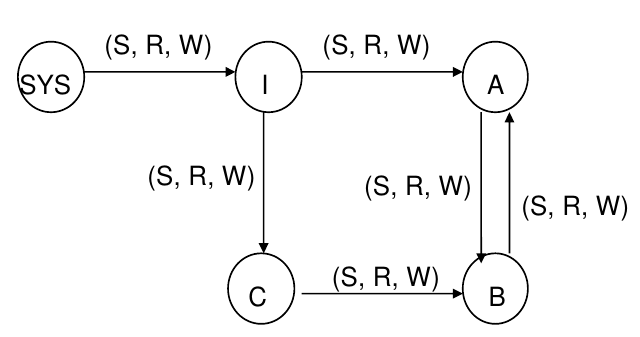
\includegraphics[scale=0.2]{grafo1.png}
			\captionof{figure}{GRANT}
		\end{minipage}
		\begin{minipage}{.3\textwidth}
			\centering
			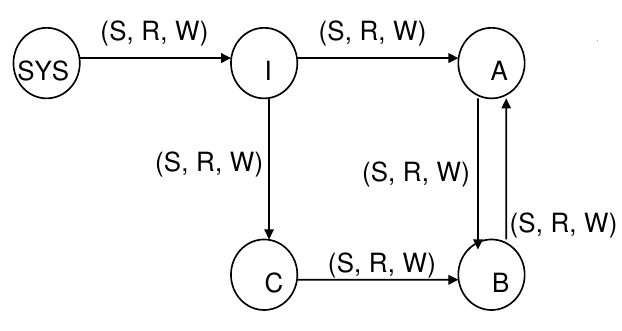
\includegraphics[scale=0.2]{grafo2.png}
			\captionof{figure}{Prima REVOKE}
		\end{minipage}
		\begin{minipage}{.3\textwidth}
			\centering
			\includegraphics[scale=0.2]{grafo3.png}
			\captionof{figure}{Seconda REVOKE}
		\end{minipage}
	\end{figure}
\end{example}

\subsection{Indici}
Gli Indici sono strutture dati che vengono create su tabelle per eseguire alcune query più velocemente. Non essendo un comando standard può avere varie sintassi:
\begin{lstlisting}[language=SQL]
	CREATE INDEX NomeIdx ON Tabella(Attributi)
	CREATE INDEX NomeIdx ON Tabella	WITH STRUCTURE = BTREE, KEY = (Attributi)
	DROP INDEX NomeIdx
\end{lstlisting}

\newpage
\subsection{Catalogo dei metadati}
Il catalogo dei metadati consiste in un insieme di tabelle di sistema. Alcuni esempi sono:
\begin{itemize}
	\item Delle \textbf{password}
	\begin{lstlisting}[language=SQL]
		PASSWORD(username, password)
	\end{lstlisting}
	\item Delle \textbf{BD}
	\begin{lstlisting}[language=SQL]
		SYSDB(dbname, creator, dbpath, remarks)
	\end{lstlisting}
	\item Delle \textbf{tabelle} e \textbf{view} (type)
	\begin{lstlisting}[language=SQL]
		SYSTABLES(name, creator, type, colcount, filename, remarks)
	\end{lstlisting}
	\item Degli \textbf{attributi}
	\begin{lstlisting}[language=SQL]
		SYSCOLUMNS(name, tbname, tbcreator, colno, coltype, lenght, default, remarks)
	\end{lstlisting}
	\item Degli \textbf{indici}
	\begin{lstlisting}[language=SQL]
		SYSINDEXES(name, tbname, creator, uniquerule, colcount)
	\end{lstlisting}
\end{itemize}
	% !TeX spellcheck = it_IT
\newpage
\section{Normalizzazione}
Dati diversi modelli relazionali e diverse possibili rappresentazioni sorge il problema di verificare se:
\begin{itemize}
	\item queste diverse rappresentazioni sono tra di loro \textbf{equivalenti}
	\item queste rappresentazioni sono di \textbf{buona qualità} (assenza di \textbf{anomalie})
\end{itemize}

\begin{definition}[Teoria della normalizzazione]
	La teoria della normalizzazione si occupa di \textbf{definire criteri formali} per giudicare l’\textbf{equivalenza} di schemi e la \textbf{qualità} di tali schemi, e di definire algoritmi per trasformare uno schema in un altro equivalente ma privo di anomalie.
\end{definition}

\subsection{Linee guida}
Ci sono quattro principali linee guida per avere una corretta progettazione:
\begin{itemize}
	\item \textbf{Semantica degli attributi}: si devono progettare schemi relazionali in modo tale che sia semplice spiegarne il significato evitando di unire attributi provenienti da più tipi di classi e tipi di associazione in una unica relazione.
	\item \textbf{Ridondanza}: si devono progettare schemi relazionali in modo che nelle relazioni non
	siano presenti anomalie di inserimento, cancellazione o modifica. Se sono presenti (e le si vuole mantenere), le si rilevi e ci si assicuri che i programmi che aggiornano la BD operino correttamente
	\item \textbf{Valori nulli}: evitare di porre in relazione di base attributi i cui valori possono essere spesso nulli. Se è inevitabile, assicurarsi che essi si presentino solo in casi eccezionali e che non riguardino una maggioranza di tuple nella relazione.
	\item \textbf{Tuple spurie}: si devono progettare schemi relazionali in modo tale che essi possano
	essere riuniti tramite giunzioni con condizioni di uguaglianza su attributi	che sono o chiavi primarie o chiavi esterne in modo da garantire che	non vengano generate tuple spurie. Evitare relazioni che contengono attributi di giunzione diversi dalle combinazioni chiave esterna-chiave primaria.
\end{itemize}

\subsubsection{Anomalie}
Le principali anomalie che si trovano sono:
\begin{itemize}
	\item \textbf{Ridondanze}
	\item Potenziali \textbf{inconsistenze}
	\item Anomalie nelle \textbf{inserzioni}
	\item Anomalie nelle \textbf{eliminazioni}
\end{itemize}

\begin{example}
	Supponiamo di avere una BD di una biblioteca
	\begin{center}
		\includegraphics[scale=0.3]{biblioteca1.png}
	\end{center}
	Questo schema presenta due anomalie:
	\begin{itemize}
		\item \textbf{Ridondanza} delle informazioni personali di un utente
		\item Impossibilità di rappresentare le informazioni sugli utenti della biblioteca che non hanno preso in prestito libri
	\end{itemize}
	Una possibile soluzione è la \textbf{decomposizione} in due relazioni:
	\begin{lstlisting}[language=SQL]
		Utenti(NomeUtente, Residenza, Telefono)
		Prestiti(NumeroLibro, Autore, Titolo, Data, NomeUtente*)
	\end{lstlisting}
	Non è la soluzione migliore per costo di operazioni ma funziona.
\end{example}

\subsubsection{Obiettivi}
L'obiettivo della normalizzazione è fornire \textbf{strumenti formali} per la progettazione di basi di dati che non presentino anomalie senza prendere in considerazione il costo delle operazioni. In particolare si occupa di:
\begin{itemize}
	\item \textbf{Equivalenza di schemi}: definire quando due schemi sono equivalenti
	\item \textbf{Qualità degli schemi}: definire quando uno schema è migliore di un altro
	\item \textbf{Trasformazione degli schemi}: trovare metodi algoritmici per ottenere da uno schema uno migliore ed equivalente
\end{itemize}

\subsubsection{Schema di relazione universale}
\begin{definition}[Schema di relazione universale]
	Assumendo come \textbf{ipotesi} che tutti i fatti sono descritti da attributi di un’unica relazione
	(relazione universale), cioè gli attributi hanno un significato globale.\\
	\textbf{Definiamo} lo schema di relazione universale U come di una base di dati relazionale ha come attributi l’unione degli attributi di tutte le relazioni della base di dati.
\end{definition}

\subsubsection{Notazione}
Di seguito la notazione di base:
\begin{itemize}
	\item \textbf{Singoli attributi}: $A,B,C, A_1, A_2, \ldots$
	\item \textbf{Insiemi di attributi}: $T,X,Y,X_1, \ldots$
	\item \textbf{Abbreviazioni}:
	\begin{itemize}
		\item $XY \equiv X \cup Y$
		\item $AB \equiv \{A, B\}$
		\item $A_1, A_2, \ldots, A_n \equiv \{A_1, A_2, \ldots, A_n\}$
		\item $XA \equiv A \cup \{A\}$
	\end{itemize} 
	\item \textbf{Schema di relazione}: $R(T)$, $r$ la sua \textbf{istanza} e $t$ l'\textbf{ennupla} dell'istanza
	\item Se $X \subseteq T$ allora $t[X]$ indica l'\textbf{ennupla} ottenuta da $T$ considerando solo gli attributi in $X$
\end{itemize}


\subsection{Dipendenze funzionali}
Informalmente, una dipendenza funzionale indica che dato un insieme di attributi, questi ne determinano in maniera univoca altri.

\begin{definition}[Dipendenza funzionale]
	Dato uno schema $R(T)$ e $X, Y \subseteq T$, una dipendenza funzionale è un vincolo su $R$ del tipo $X \to Y$ se:
	\begin{itemize}
		\item $\forall r$ istanza valida di $R$
		\item $\forall t_1, t_2 \in r . t_1[X] = t_2[X] \Rightarrow t_1[Y]=t_2[Y]$
	\end{itemize}
\end{definition}
\newpage
\begin{example}
	Data la seguente tabella
	\begin{table}[!h]
		\centering
		\begin{tabular}{|c|c|}
			\hline
			\textbf{Matricola} & \textbf{Cognome}\\
			\hline
			1 & Rossi \\
			\hline
			2 & Verdi \\
			\hline
			3 & Rossi \\
			\hline
			4 & Viola \\
			\hline
		\end{tabular}
	\end{table}
	esiste la dipendenza funzionale $\text{Matricola} \to \text{Cognome}$
\end{example}

\begin{note}
	Essendo definite solo all'interno di una relazione non possono esistere fra attributi di relazioni diverse.
\end{note}
\begin{note}
	Sono proprietà \textbf{intensionali}, quindi legate al significato dei fatti. Non è possibile dedurle dall'osservazione di alcune istanze.
\end{note}

\begin{definition}[Dipendenza funzionale atomica]
	Ogni DF del tipo $X \to A_1, A_2, \ldots, A_n$ si può scomporre in $X\to A_1, X \to A_2, \ldots, X\to A_n$. DF del tipo $X \to A$ sono dette \textbf{atomiche}.
\end{definition}

\begin{example}
	Dato lo schema
	\begin{equation*}
		\text{DotazioniLibri}(\text{CodiceLibro}, \text{NomeNegozio}, \text{IndNegozio}, \text{Titolo}, \text{Quantità})
	\end{equation*}
	la dipendenza funzionale
	\begin{equation*}
		\text{CodiceLibro}, \text{NomeNegozio}\to \text{IndNegozio}, \text{Titolo}, \text{Quantità}
	\end{equation*}
	si può scomporre in
	\begin{align*}
		& \text{CodiceLibro}, \text{NomeNegozio}\to \text{IndNegozio} \\
		& \text{CodiceLibro}, \text{NomeNegozio}\to \text{Titolo}\\
		& \text{CodiceLibro}, \text{NomeNegozio}\to \text{Quantità}
	\end{align*}
\end{example}

\begin{definition}[Dipendenza funzionale banale]
	Una DF $X \to A$ è detta \textbf{banale} se $A \in X$.
\end{definition} 

\subsubsection{Chiavi}
Le dipendenze funzionali sono una generalizzazione del vincolo di chiave e superchiave. Infatti, dato uno schema $R(T)$, $X,Y \subseteq T$ e $r$ istanza di $R$, se $r \models X \to Y$ allora se $X$
\begin{itemize}
	\item \textbf{Non} è \textbf{superchiave} allora ho un'\textbf{anomalia}
	\item È \textbf{superchiave}, allora $\forall r . r\models X \to T$
	\item È \textbf{chiave}, allora $\forall r. r\models X \to T$ e $X \to T$ è una DF \textbf{completa}
\end{itemize}

\subsubsection{Utilizzo}
Le dipendenze funzionali vengono utilizzate per specificare il significato dei fatti rappresentati in uno schema trovando eventuali anomalie e normalizzandolo. Per questo motivo da ora saranno incluse nella definizione:
\begin{equation}
	R(T,F)
\end{equation}

\paragraph{Dipendenze derivate}
Dato uno schema $R(T,F)$, le sue istanza soddisfano le DF e anche quelle derivabili da esse. Ad esempio dato
\[
R(T,F=\{X \to Y, X \to Z\}) \qquad X,Y,Z \subseteq T, W \subseteq X
\]
allora anche $X \to W$ e $X \to YZ$ saranno soddisfatte:
\begin{itemize}
	\item la prima è ovvia in quanto $W$ è sottoinsieme di $X$
	\item se $t_1[X] = t_2[X]$  allora $t_1[Y] = t_2[Y] \land t_1[Z] = t_2[Z]$ e quindi $t_1[YZ] = t_2[YZ]$
\end{itemize}
\begin{definition}[Implicazione di dipendenze]
	Dato $R(T)$ e dato $F$, diciamo che $F \models X \to Y$ ($F$ implica logicamente $X \to	Y$), se ogni istanza $r$ di $R(T)$ che soddisfa $F$ soddisfa anche $X \to Y$.
\end{definition}

\paragraph{Assiomatizzazione}
Sia $RI$ un insieme di regole di inferenze per $F$, ovvero per derivare altre DF a partire da $F$. Indichiamo con $F \vdash X \to Y$ il fatto che $X \to Y$ sia derivabile da $F$ usando $RI$. L'insieme $RI$ è:
\begin{itemize}
	\item \textbf{Corretto}: se $X \to Y$ è derivabile da $F$ allora ogni istanza che soddisfa $F$ soddisfa anche $X \to Y$
	\begin{equation*}
		F \vdash X \to Y \Longrightarrow F \models X \to Y
	\end{equation*}
	\item \textbf{Completo}: se ogni istanza che soddisfa $F$ soddisfa anche $X \to Y$ implica che $X \to Y$ è derivabile da $F$
	\begin{equation*}
		F \models X \to Y \Longrightarrow F \vdash X \to Y
	\end{equation*}
\end{itemize}

\paragraph{Regole di inferenza}
Gli assiomi di Armstrong (1974) sono il più noto insieme \textbf{corretto} e \textbf{completo} di regole di inferenza per DF:
\begin{itemize}
	\item \textbf{Riflessività}
	\begin{equation}
		Y \subseteq X \Longrightarrow X \to Y
	\end{equation}
	\item \textbf{Arricchimento}
	\begin{equation}
		X \to Y, Z \subseteq T \Longrightarrow XZ \to YZ
	\end{equation}
	\item \textbf{Transitività}
	\begin{equation}
		X \to Y, Y \to Z \Longrightarrow X \to Z
	\end{equation}
\end{itemize} 

\begin{definition}[Derivazione]
	Una \textbf{derivazione} di $f$ da $F$ è una sequenza finita $f_1, \ldots, f_m$ di dipendenze dove $f_m = f$ e ogni $f_i$ è un elemento di $F$ oppure è ottenuta dalle	precedenti dipendenze delle derivazione $f_1, \ldots, f_{i-1}$ usando regole di inferenza.\\
	Una \textbf{sottosequenza} $f_1, \ldots, f_k$ per una derivazione $f_1,\ldots, f_m$ è anch’essa	una derivazione, quindi $F \vdash f_k \forall k = 1, \ldots, m$.
\end{definition}
Sia $F$ un insieme di DF, diremo che $X \to Y$ sia \textbf{derivabile} da $F$ ($F \vdash X \to Y$), se $X \to Y$ può essere inferito da $F$ usando gli assiomi di Armstrong.\\
Vediamo altre regole di derivazione ottenute dagli assiomi di Armstrong:
\begin{itemize}
	\item \textbf{Unione}: $\{X \to Y, X \to Z\} \vdash X \to YZ$
	\begin{enumerate}
		\item  $X \to Y$ per ipotesi
		\item $X \to XY$ per arricchimento da 1
		\item $X \to Z$ per ipotesi
		\item $XY \to YZ$ per arricchimento da 3
		\item $X \to YZ$ per transitività da 2, 4
	\end{enumerate}
	\item \textbf{Decomposizione}: $\{X \to YZ\} \vdash X \to Y$
	\begin{enumerate}
		\item $X \to YZ$ per ipotesi
		\item $YZ \to Y$ per riflessività da $Y \subseteq YZ$
		\item $ X \to Y$ per transitività da 1, 2
	\end{enumerate}
	\item \textbf{Indebolimento}: $\{X \to Y\} \vdash XZ \to Y$
	\begin{enumerate}
		\item $X \to Y$ per ipotesi
		\item $XZ \to X$ per riflessività da $X \subseteq XZ$
		\item $ XZ\to Y$ per transitività da 2, 1
	\end{enumerate}
	\item \textbf{Identità}: $\{\} \vdash X \to X$
\end{itemize}
\newpage
\begin{theorem}
	Gli assiomi di Armstrong sono \textbf{corretti} e \textbf{completi}.
\end{theorem}
\begin{proof}
	Se una dipendenza è derivabile con gli assiomi di Armstrong allora è anche implicata logicamente (correttezza degli assiomi), e viceversa se una dipendenza è implicata logicamente allora è anche derivabile dagli assiomi (completezza degli assiomi).
	\begin{itemize}
		\item Correttezza
		\begin{equation}
			\forall f \qquad F \vdash f \Longrightarrow F \models f
		\end{equation}
		\item Completezza
		\begin{equation}
			\forall f \qquad F \models f \Longrightarrow F \vdash f
		\end{equation}
	\end{itemize}
\end{proof}

 \subsubsection{Chiusura}
 La \textbf{chiusura} è l’insieme di DF $X \to Y$ derivabili da $F$.
\begin{definition}[Chiusura]
	Dato un insieme $F$ di DF, la sua chiusura, denotata con $F^+$ è
	\begin{equation}
		F^+ = \{ X \to Y \vert F \vdash X \to Y\}
	\end{equation}
\end{definition}

La chiusura di $X$ rispetto ad $F$ è l’insieme di attributi determinati da $X$ tra quelli delle DF derivabili da $F$.
\begin{definition}[Chiusura]
	Dato $R(T, F)$, e $X \subseteq T$, la chiusura di $X$ rispetto a $F$, denotata con $X_F^+$, (o $X^+$, se $F$ è chiaro dal contesto) è
	\begin{equation}
		X_F^+ = \{A_i \in T \vert F \vdash X \to A_i \}
	\end{equation}
\end{definition}

\paragraph{Problema dell'implicazione}
Il problema dell'implicazione consiste nel decidere se una DF $V \to W$ appartiene a $F^+$. La sua risoluzione con l’algoritmo di generare $F^+$ applicando ad $F$ ripetutamente gli assiomi di Armstrong ha una complessità esponenziale rispetto al numero di attributi dello schema.\\
Un algoritmo più semplice si basa sul seguente teorema:
\begin{theorem}
	Da DF $X \to Y$ è derivabile da $F$ se e solo se $Y$ è sottoinsieme	della chiusura di $X$ rispetto a $F$.
	\begin{equation}
		F\vdash X \to Y \Leftrightarrow Y \subseteq X_F^+.
	\end{equation}
\end{theorem}

\begin{lstlisting}[language=SQL, mathescape]
	input		R(T,F), X $\subseteq$ T
	output	  $X^+$
	begin
		$X^+$ = X
		while ($X^+$ cambia) do
			for $W \to V$ in F with $W \subseteq X^+$ and $V \subsetneq X^+$
				do $X^+ = X^+ \cup V$
	end
\end{lstlisting}
L'algoritmo \textbf{termina} perché gli attributi sono di numero finito e per dimostrare la \textbf{correttezza} si dimostra per induzione che $X_F^+ = X^+$.

\paragraph{Definizione di chiavi}
\begin{definition}[Superchiave]
	Dato lo schema $R(T, F)$, un insieme di attributi $W \subseteq T$ è	una superchiave di $R$ se $W \to T \in F^+$.
\end{definition}

\begin{definition}[Chiave]
	Dato lo schema $R(T, F)$, un insieme di attributi $W \subseteq T$ è	una chiave di $R$ se $W$ è una superchiave e non esiste un sottoinsieme stretto di $W$ che sia superchiave di $R$.
\end{definition}

\begin{definition}[Attributo primo]
	Dato lo schema $R(T, F)$, un attributo $A \in T$ si dice attributo primo se e solo se appartiene ad almeno una chiave, altrimenti si dice non primo.
\end{definition}

\subparagraph{Trovare tutte le chiavi}
L’algoritmo per trovare tutte le chiavi si basa su due proprietà:
\begin{enumerate}
	\item Se un attributo $A$ di $T$ non appare a destra di alcuna dipendenza in $F$, allora $A$ appartiene ad ogni chiave di $R$ (altrimenti non può essere determinato)
	\item Se un attributo $A$ di $T$ appare a destra di qualche dipendenza in $F$, ma non appare a sinistra di alcuna dipendenza non banale, allora $A$ non appartiene ad alcuna chiave.
\end{enumerate}

Sia $X$ l’insieme degli attributi che non appaiono a destra di alcuna dipendenza in $F$. Da 1. segue che se $X^+ = T$, allora $X$ è una chiave di $R$ ed è anche l’unica possibile. Altrimenti, occorre aggiungere a $X$ altri attributi. Per 2. basta aggiungere gli attributi $W$ di $T$ che appaiono a destra di qualche dipendenza e a sinistra di qualche altra, uno alla volta evitando di aggiungere quelli che sono già in $X^+$ o quelli che producono un $X’$ che contiene una chiave già trovata.

\begin{lstlisting}[language=SQL, mathescape]
	input		  R(T,F)
	output		Insieme di tutte le chiavi
	
	begin
		NoDes := $T-\cup_{X\to A \in F}A$;
		SinDes := $\cup_{X \to A \in F}X \cap \cup_{X\to A \in F}A$;
		Candidati := [NoDes::(SinDes)];
		Chiavi := [];
		while (Candidati non vuoto) do
			begin
				X::(Y) := first(Candidati);
				Candidati := rest(Candidati);
				if not some K in Chiavi with $K \subset X$
				then if $X^+ = T$ then Chiavi := Chiavi + X;
					else begin
						$A_1, \ldots, A_n$ := $Y - X^+$;
						for i in $1, \ldots, n$ do Candidati = Candidati.append($XA_i$::($A_{i+1}, \ldots, A_n$))
					end
			end
	end
\end{lstlisting}

\begin{note}
	Il problema di trovare tutte le chiavi di una relazione richiede un algoritmo di complessità \textbf{esponenziale}.
\end{note}

\begin{note}
	Il problema di controllare se un attributo è primo è \textbf{NP-completo}.
\end{note}

\subsubsection{Copertura canonica}
\begin{definition}[Copertura]
	Due insiemi di DF, $F$ e $G$, sullo schema $R$ sono	equivalenti ($F\equiv G$) se e solo se $F^+ = G^+$. Se $F \equiv G$, allora $F$ è una copertura di $G$ e viceversa.
\end{definition}

\begin{definition}[Attributo estraneo]
	Sia $F$ un insieme di DF. Data una $X \to Y \in F$, si dice che $X$ contiene un attributo estraneo $A_i$
	se e solo se $(X - \{A_i\}) \to Y \in F^+$, cioè $F \vdash (X - \{A_i\}) \to Y$.
\end{definition}

\begin{example}[Attributo estraneo]
	Sia
	\begin{equation*}
		F = \{AB \to C, A \to B\}
	\end{equation*}
	Calcoliamo $A^+ = ABC$ e vediamo che $C$ dipende solo da $A$ e di conseguenza $B$ è \textbf{estraneo} in $AB \to C$.
\end{example}

\begin{definition}[Dipendenza ridondante]
	$X \to Y$ è una dipendenza ridondante se e solo se $(F - \{X \to Y\})^+ = F ^+$, equivalentemente $F - \{X \to Y\} \vdash X \to Y$.
\end{definition}

\begin{example}[Dipendenza ridondante]
	Sia
	\begin{equation*}
		F = \{B \to C, B \to A, C \to A\}
	\end{equation*}
	$B \to A$ è \textbf{ridondante} poiché possiamo dedurla da $B \to C$ e $C \to A$.
\end{example}

\newpage
\begin{definition}[Copertura canonica]
	$F$ è detta copertura canonica se e solo se:
	\begin{itemize}
		\item la parte destra di ogni DF in $F$ è un attributo, ovvero tutte le DF sono \textbf{atomiche}
		\item non esistono \textbf{attributi estranei}
		\item nessuna dipendenza in $F$ è \textbf{ridondante}
	\end{itemize}
\end{definition}

\begin{theorem}[Esistenza copertura canonica]
	Per ogni insieme di dipendenze $F$ esiste una copertura canonica.
\end{theorem}

Per calcolare la copertura canonica si può applicare il seguente algoritmo:
\begin{enumerate}
	\item Trasformare le dipendenze nella forma $X \to A$: si sostituisce l’insieme dato con quello equivalente che ha tutti i secondi membri costituiti da singoli attributi (dipendenze atomiche)
	\item Eliminare gli attributi estranei: per ogni dipendenza si verifica se esistono attributi eliminabili dal primo membro
	\item Eliminare le dipendenze ridondanti: per ogni dipendenza si verifica se può essere eliminata
\end{enumerate}

\subsection{Decomposizione di schemi}
L’approccio da seguire per eliminare \textbf{anomalie} da uno schema mal definito, è quello di \textbf{decomporlo} in schemi più piccoli che godono di particolari proprietà (\textbf{forme normali}), ma sono in qualche senso equivalenti allo schema originale. L’intuizione è che si devono “estrarre” gli attributi che sono determinati da attributi non chiave ovvero “creare uno schema per ogni funzione”.\\

\noindent Le \textbf{ridondanze} sui dati possono essere:
\begin{itemize}
	\item \textbf{Concettuali}: non ci sono duplicazioni dello stesso dato ma sono memorizzate informazioni che possono essere ricavate da altre già contenute nella BD
	\item \textbf{Logiche}: esistono duplicazioni sui dati che possono generare anomalie
\end{itemize}

\begin{definition}[Decomposizione]
	Dato uno schema $R(T)$,	$\rho = \{R_1(T_1),\ldots, R_k(T_k)\}$ è una decomposizione di $R$ se e solo se $T_1 \cup  \ldots \cup T_k = T$.
\end{definition}

\begin{example}[Decomposizione]
	Prendiamo la relazione
	\begin{lstlisting}[language=SQL]
		Articoli(Kit, Componente, Tipo, QuantComp, PrezzoComp, Fornitore, PrezzoTot)
	\end{lstlisting}
	\begin{table}[!h]
		\centering
		\begin{tabular}{|c|c|c|c|c|c|c|}
			\hline
			\textbf{Kit} & \textbf{Componente} & \textbf{Tipo} & \textbf{QuantComp} & \textbf{PrezzoComp} & \textbf{Fornitore} & \textbf{PrezzoTot} \\
			\hline
			Libreria & Legno & Noce & 50 & 10 & A & 4400 \\
			\hline
			Libreria & Bulloni & Acciaio & 200 & 1 & B & 4400 \\
			\hline
			Libreria & Vetro & Cristallo & 3 & 50 & C & 4400 \\
			\hline
			Scaffale &Legno & Mogano & 37 & 15 & A & 555 \\
			\hline
			PC & Bulloni & Acciaio & 25 & 1 & B & 700 \\
			\hline
			PC & Tastiera & A3000 & 3 & 30 & D & 700\\
			\hline
			PC & Mouse & B2000 & 5 & 45 & D & 700 \\
			\hline
			$\ldots$ & $\ldots$ & $\ldots$ & $\ldots$ & $\ldots$ & $\ldots$ & $\ldots$ \\
			\hline
		\end{tabular}
	\end{table}
	Identifichiamo le \textbf{ridondanze}:
	\begin{itemize}
		\item \textbf{PrezzoTot} è ripetuto in ogni tupla riferita allo stesso \textbf{Kit}
		\item \textbf{PrezzoComp} è ripetuto in ogni tupla che ha lo stesso valore di \textbf{Tipo} e \textbf{Fornitore}
		\item \textbf{Componente} è ripetuto in ogni tupla che ha lo stesso \textbf{Tipo}
	\end{itemize}
	\newpage
	\noindent Scriviamo poi le \textbf{dipendenze} derivate:
	\begin{itemize}
		\item \textbf{Tipo} $\to$ \textbf{Componente}
		\item \textbf{Kit} $\to$ \textbf{PrezzoTot}
		\item \textbf{Kit}, \textbf{Tipo} $\to$ \textbf{PrezzoComponente}, \textbf{QuantComp}, \textbf{Fornitore}
	\end{itemize}
	questo ci porta ad avere la seguente decomposizione
	\begin{table}[!h]
		\centering
		\begin{tabular}{|c|c|c|c|c|}
			\hline
			\textbf{Kit} & \textbf{Tipo} & \textbf{QuantComp} & \textbf{PrezzoComp} & \textbf{Fornitore} \\
			\hline
		\end{tabular}\newline
		\begin{tabular}{|c|c|}
			\hline
			\textbf{Kit} & \textbf{PrezzoTot} \\
			\hline
		\end{tabular}
		\begin{tabular}{|c|c|}
			\hline
			\textbf{Tipo} & \textbf{Componente} \\
			\hline
		\end{tabular}
	\end{table}
\end{example}

\noindent Una decomposizione dovrebbe sempre soddisfare le seguenti qualità:
\begin{itemize}
	\item Decomposizione \textbf{senza perdita} che garantisce la ricostruzione delle informazioni originarie senza generazione di tuple spurie
	\item \textbf{Conservazione delle dipendenze} che garantisce il mantenimento dei	vincoli di integrità (di dipendenza funzionale) originari
\end{itemize}

\subsubsection{Conservazione dei dati}
Per una decomposizione che preserva i dati, ogni istanza valida $r$ della relazione di partenza deve essere uguale alla giunzione naturale della sua proiezione sui $T_i$.
\begin{definition}[Conservazione dei dati]
	$\rho = \{R_1(T_1), \ldots, R_k(T_k)\}$ è una decomposizione di uno schema $R(T)$ che preserva i dati se e solo se per ogni istanza valida $r$ di $R$:
	\begin{equation}
		r = (\pi_{T1}r) \Join (\pi_{T_2}r) \Join \ldots \Join (\pi_{T_k}r)
	\end{equation}
\end{definition}
\paragraph{Perdita di informazione}
Una \textbf{perdita di informazione} è quando, proiettando una relazione sui sottoschemi e poi facendo la giunzione, si ottengono più ennuple di quante ce ne fossero nella relazione originaria.
\begin{theorem}[Perdita di informazione]
	Se $\rho = \{R_1(T_1), \ldots, R_k(T_k)\}$ è una decomposizione di $R(T)$, allora per ogni istanza $r$ di $R$
	\begin{equation}
		r \subseteq (\pi_{T_1}r) \Join (\pi_{T_2}r) \Join \ldots \Join (\pi_{T_k}r)
	\end{equation}
\end{theorem}

Uno schema $R(X)$ si decompone \textbf{senza perdite} negli schemi $R_1(X_1)$ ed $R_2(X_2)$ se, per ogni possibile istanza $r$ di $R(X)$, il join naturale delle proiezioni di $r$ su $X_1$ ed $X_2$ produce la tabella di partenza, cioè non contiene ennuple spurie.
\begin{equation*}
	\prescript{}{X_1}{(r)} \Join \prescript{}{X_2}{(r)} = r
\end{equation*}

\begin{example}[Perdita di informazione]
	Supponiamo di avere lo schema
	\begin{lstlisting}[language=SQL]
		StudentiEdEsami(Matricola, Nome, Provincia, AnnoNascita, Materia, Voto)
	\end{lstlisting}
	e lo decomponiamo in
	\begin{lstlisting}[language=SQL]
		Studenti(Matricola, Nome, Provincia, AnnoNascita),
		Esami(Nome, Materia, Voto)
	\end{lstlisting}
	Quando andiamo a fare la \textbf{giunzione naturale}, si creano tuple che prima non esistevano. Basta immaginare cosa succederebbe se due studenti con lo stesso nome avessero fatto esami diversi.
\end{example}

\begin{theorem}[Decomposizione senza perdita]
	Se l’insieme degli attributi comuni alle due relazioni $(X1 \cap X2)$ è chiave per almeno una delle due relazioni decomposte allora la decomposizione è senza perdita.
\end{theorem}

\begin{proof}
	Supponiamo $r$ sia una relazione sugli attributi $ABC$ e consideriamo le sue proiezioni $r_1$ su $AB$ e $r2$ su $AC$. Supponiamo che $r$ soddisfi la dipendenza funzionale $A \to C$. Allora $A$ è chiave per $r$ su $AC$ e quindi non ci sono in tale proiezione due tuple diverse sugli stessi valori di $A$.
\end{proof}

\paragraph{Decomposizione binaria}
\begin{theorem}
	Sia $R(T, F)$ uno schema di relazione, la decomposizione $\rho = \{R_1(T_1), R_2 (T_2)\}$ preserva i dati se e solo se $T_1 \cap T_2 \to T_1 \in F^+$ oppure $T_1 \cap T_2 \to T_2 \in F^+$.
\end{theorem}

\subsubsection{Conservazione delle dipendenze}
Una decomposizione preserva le dipendenze se ciascuna delle dipendenze funzionali dello schema originario coinvolge attributi che compaiono tutti insieme in uno degli schemi decomposti.

\paragraph{Proiezione di una dipendenza funzionale}
\begin{definition}[Proiezione di una DF]
	Dato lo schema $R(T, F)$, e $T_1 \subseteq T$, la proiezione di $F$ su $T_1$ è $\pi_{T_1} (F) = \{X \to Y \in F^+ \vert XY \subseteq T_1\}$.
\end{definition}

\noindent Un algoritmo per il calcolo della proiezione è il seguente
\begin{lstlisting}[language=SQL, mathescape]
	for each $Y \subseteq T_1$ do ($Z:= Y^+$; output $Y \to Z \cap T_1$)
\end{lstlisting}

\begin{example}[Proiezione di DF]
	Siano
	\begin{equation*}
		R(A,B,C) \qquad\qquad F=\{A \to B, B \to C, C \to A\}
	\end{equation*}
	Abbiamo le seguenti proiezioni
	\begin{align*}
		& \pi_{AB}(F) \equiv \{A \to B, B \to A\}\\
		& \pi_{AC}(F) \equiv \{A \to C, C \to A\}
	\end{align*}
\end{example}

\begin{definition}[Conservazione delle dipendenze]
	Dato lo schema $R(T, F)$, la decomposizione $\rho = \{R_1, \ldots, R_n\}$ preserva le dipendenze se e solo se l’unione delle dipendenze in $\pi_{T_i}(F)$ è una copertura di $F$.
\end{definition}

\begin{note}
	Il problema di stabilire se una decomposizione conserva le dipendenze è di complessità \textbf{polinomiale}.
\end{note}

\begin{theorem}
	Sia $\rho = \{R_i(T_i, F_i)\}$ una decomposizione di $R(T, F)$ che preservi le dipendenze e tale che un $T_j$ sia una superchiave per $R$. Allora $\rho$ preserva i dati.
\end{theorem}

\subsection{Forme normali}
Una forma normale è una \textbf{proprietà} di una base di dati relazionale che ne garantisce la \textbf{qualità}, cioè l'assenza di determinati difetti.\\
Le forme normali sono:
\begin{itemize}
	\item \textbf{Prima} forma normale: impone una restrizione sul tipo di una relazione: ogni attributo ha un tipo elementare
	\item \textbf{Seconda} forma normale: impone una restrizione sulle dipendenze
	\item \textbf{Terza} forma normale: impone una restrizione sulle dipendenze
	\item \textbf{BCNF}: la più naturale e restrittiva
\end{itemize}

\subsubsection{Boyce-Cobb Normal Form}
Una relazione $r$ è in BCNF se, per ogni DF non banale $X \to Y$ definita su di essa, $X$ contiene una chiave $K$ di $r$, ovvero $X$ è una \textbf{superchiave}. La forma normale richiede che i concetti in una relazione siano omogenei (solo proprietà direttamente associate alla chiave).

\begin{definition}[BCNF]
	$R(T, F)$ è in BCNF se e solo se per ogni $X \to A \in F^+$ non banale ($A \notin X$), $X$ è una \textbf{superchiave}.
\end{definition}
\begin{theorem}
	$R(T, F)$ è in BCNF se e solo se per ogni $X \to A \in F$ non banale, $X$ è una \textbf{superchiave}.
\end{theorem}
\begin{corollaries}
	$R(T, F)$ con $F$ in copertura canonica è in BCNF se e solo se per ogni DF atomica non banale $X \to A\in F$, $X$ è una \textbf{superchiave} (ovvero è una chiave).
\end{corollaries}

Quindi un algoritmo per controllare se uno schema di relazione è in BCNF ha \textbf{complessità} $O(ap^2)$, dove $a$ è il numero di attributi in $T$ e $p$ è il numero di DF in $F$.

\paragraph{Algoritmo di analisi}
Questo algoritmo prevede che $R(T, F)$ venga decomposta in: $R_1(X, Y)$ e $R_2(X, Z)$ e su di esse si ripeta il procedimento.
\begin{lstlisting}[language=SQL, mathescape]
	Input		   $R(T, F)$ con $F$ copertura canonica
	Output		$\rho= \{R_1, R_2 , R_m \}$ decomposizione in BCNF che preserva i dati
	$\rho = \{R_1(T_1, F_1)\}$
	while esiste in $\rho$ una $R_i(T_i, F_i)$ non in BCNF per la DF $X \to A$
	do
		n = n + 1 # incrementa contatore relazioni
		$T_a = X^+$ # chiusura di $X$
		$F_a = \pi_{T_a}(F_i)$ # proiezione DF rispetto a $T_a$
		$T_b = T_i - X^+ + X$ # rimozione da attributi non in $X$ ma nella sua chiusura
		$F_b = \pi{T_b} (F_i)$ # proiezione DF rispetto a $T_b$
		$\rho = \rho - R_i + \{ R_i<T_a, F_a>, R_n< T_b, F_b > \}$ # rimuove $R$ non BCNF per $X \to A$ e inserisce quelle corrette
	end
\end{lstlisting}
Questo algoritmo \textbf{NON} garantisca la conservazione delle dipendenze ma preserva i dati.

\begin{example}[Applicazione dell'algoritmo]
	Prendiamo
	\begin{equation*}
		R(ABCDE, F=\{CE \to A, D \to E, CB \to E, CE \to B\})
	\end{equation*}
	e applichiamo l'algoritmo:
	\begin{enumerate}
		\item Consideriamo $F_1 = (CE \to A)$. $CE^+ = CEAB$, quindi $CE$ non è chiave (manca $D$). Decomponiamo in:
		\begin{itemize}
			\item $R_1(CEAB)$: gli attributi di $CE^+$
			\item $R_2(CED)$: l'attributo mancante $D$ e la chiave esterna $CE$
		\end{itemize}
		\item Proiettiamo le dipendenze funzionali
		\begin{itemize}
			\item $R1(CEAB, \{CE \to A, CB \to E, CE \to B\})$
			\item $R2(CED, \{D \to E\})$
		\end{itemize}
		\item Consideriamo:
		\begin{itemize}
			\item $CE \to A$ e $CE \to B$, $CE^+=CEAB$
			\item $CB \to E$, $CB^+ = CEAB$
		\end{itemize}
		quindi $R_1$ è in CBNF
		\item Consideriamo $D \to E$, $D^+ = DE$ quindi $D$ non è chiave (manca $C$). Decomponiamo in:
		\begin{itemize}
			\item $R_3(DE)$
			\item $R_4(DC)$
		\end{itemize}
		\item La decomposizione ottenuta è
		\begin{equation*}
			\{R_1(CBEA), R_3(DE), R_4(DC)\}
		\end{equation*}
		e preserva dati e dipendenze
	\end{enumerate}
\end{example}
\newpage
\subsubsection{Terza forma normale}
\begin{definition}[Terza forma normale]
	$R(T, F)$ è in terza forma normale se per ogni $X \to A \in F^+$, con $A \notin X$, $X$ è una superchiave o $A$ è primo.
\end{definition}
 A differenza della BCNF, la terza forma normale \textbf{ammette} dipendenze \textbf{non banali} e da \textbf{non da chiave} se gli attributi a destra sono primi (possibili anomalie).
 
 \begin{theorem}
 	$R(T, F)$ è in terza forma normale se per ogni $X \to A \in F$ non banale, allora $X$ è una superchiave, oppure $A$ è primo (ovvero è contenuto in almeno una chiave).
 \end{theorem}
 
Ogni schema $R(T, F)$ ammette sempre una decomposizione che preserva i dati, preserva le dipendenze, ed è in 3NF. Tale decomposizione può essere ottenuta in \textbf{tempo polinomiale}.\\
Lo \textbf{svantaggio} sta nel fatto che, essendo la 3NF meno restrittiva della BCNF, accetta anche schemi che presentano delle \textbf{anomalie} e quindi certifica meno lo qualità dello schema ottenuto.
In particolare tollera \textbf{ridondanze} sui dati.

\paragraph{Algoritmo di sintesi}
L'idea è che dato un insieme di attributi $T$ ed una copertura canonica $G$, si partiziona $G$ in gruppi $G_i$ tali che tutte le dipendenze in ognuno hanno la stessa parte sinistra. Quindi, da ogni $G_i$, si definisce uno schema di relazione composto da tutti gli attributi che vi appaiono, la cui chiave, detta \textbf{chiave sintetizzata}, è la parte sinistra comune.

\begin{lstlisting}[language=SQL, mathescape]
	Input		   Un insieme $R$ di attributi e un insieme $F$ di dipendenze su $R$
	Output		Una decomposizione $\rho = \{S_i\}_{i=1\ldots n}$ di R tale che preservi dati e dipendenze e ogni $S_i$ sia in 3NF, rispetto alle proiezioni di $F$ su $S_i$
	
	begin
		Passo 1. Trova una copertura canonica $G$ di $F$ e poni $\rho = \{\}$
		Passo 2. Sostituisci in $G$ ogni insieme $X \to A_1, \ldots , X \to A_h$ di dipendenze con lo stesso determinante, con la dipendenza $X \to A_1 \ldots A_h$
		Passo 3. Per ogni dipendenza $X \ldots Y$ in $G$, metti uno schema con attributi $XY$ in $\rho$
		Passo 4. Elimina ogni schema di $\rho$ contenuto in un altro schema di $\rho$
		Passo 5. Se la decomposizione non contiene alcuno schema i cui attributi costituiscano una superchiave per $R$, aggiungi ad essa lo schema con attributi $W$, con $W$ una chiave di $R$
	end
\end{lstlisting}

\subsection{Dipendenze multivalore}
Esistono dipendenze di tipo non funzionale che di conseguenza non possono essere risolte dalla BCNF. Queste si presentano ogni volta che in una relazione si rappresentano \textbf{proprietà multivalore indipendenti}.\\
Le anomalie non dipendono solamente dal fatto che esista una proprietà multivalore ma dal fatto che questa stia con proprietà semplici o multivalore indipendenti.\\
Per evitare queste anomalie è stato necessario introdurre la \textbf{quarta forma normale} con relativo algoritmo.
	% !TeX spellcheck = it_IT
\newpage
\section{DBMS}
Un DBMS è un sistema software che gestisce grandi quantità di dati \textbf{persistenti} e \textbf{condivisi}. Questo implica che deve essere \textbf{efficiente} e garantire \textbf{affidabilità} (fault tolerance).
\begin{center}
	\includegraphics[scale=0.4]{dbms.png}
\end{center}

\subsection{Memorie}
La memoria di un sistema di calcolo organizzato è divisa in livelli: da quelle più piccole, costose e veloci a quelle grandi, economiche e lente.\\
Le prestazioni si misurano in \textbf{tempo di accesso}, che è determinato da \textbf{latenza} (tempo di accesso al primo byte) e \textbf{tempo di trasferimento} dei dati:
\begin{equation}
	T_{\text{accesso}} = \text{latenza} + \frac{\text{dimDati}}{\text{velTransfer}}
\end{equation}

\begin{center}
	\includegraphics[scale=0.3]{memorie.png}
\end{center}
In una BD, considerate le dimensioni, risiede di solito su \textbf{dischi} e i dati vengono poi trasferiti a \textbf{blocchi} (o pagine) nella memoria centrale per essere elaborati.
\subsubsection{Hard disk}
Un hard disk (HD) è un dispositivo elettro-meccanico per la conservazione di informazioni sotto forma magnetica, su supporto rotante a forma di piatto su cui agiscono delle testine di lettura e scrittura.\\
Un’unità a dischi contiene una pila di dischi metallici che ruota a velocità costante ed alcune testine di lettura che si muovono radialmente al disco.
\begin{center}
	\includegraphics[scale=0.3]{hdd.png}
\end{center}
Una \textbf{traccia} è organizzata in \textbf{settori} di dimensione fissa. Questi sono a loro volta raggruppati logicamente in \textbf{blocchi}, che sono l'unità di trasferimento.

\begin{note}
	Negli hard disk è fondamentale la \textbf{località}: se i settori sono vicini si impiega molto meno tempo.
\end{note}

\subsubsection{Pagina}
Un blocco o pagina è una sequenza contigua di settori su una traccia e costituisce l'unità per il trasferimento dei dati. Tipicamente è grande da $4$KB a $64$KB. Più sono piccole e più operazioni servono ma più grandi sono è più serve tempo per caricarle e si rischia frammentazione.\\
Il \textbf{tempo di trasferimento} $T_t$ di una pagina dipende dalla dimensione della pagina $P$ e dal transfer rate $T_r$.\\
La struttura di una pagina si divide in:
\begin{itemize}
	\item \textbf{Fisica}: un insieme di dimensione fissa di caratteri
	\item \textbf{Logica}: contiene informazioni di servizio e le stringhe che rappresentano i record
\end{itemize}
In un DBMS la struttura tipica di una pagina è la seguente
\begin{center}
	\includegraphics[scale=0.5]{pagina1.png}
\end{center}
La \textbf{directory} contiene un puntatore per ogni record nella pagina. In questo modo l'\textbf{identificatore di un record} (RID) nel DB è formato da:
\begin{itemize}
	\item \textbf{PID}: identificatore della pagina
	\item \textbf{Slot}: posizione all'interno della pagina
\end{itemize}
Garantendo così un'individuazione veloce e la riallocazione senza modifica del RID.
\begin{center}
	\includegraphics[scale=0.5]{pagina2.png}
\end{center}

\subsubsection{Gestore memoria permanente}
Fornisce un’\textbf{astrazione} della memoria permanente in termini di insiemi di file logici di pagine fisiche di registrazioni (blocchi), nascondendo le caratteristiche dei dischi e del sistema operativo.

\subsubsection{Gestore del buffer}
Il gestore del buffer si preoccupa del trasferimento delle pagine tra la memoria temporanea e la memoria permanente, offrendo una visione della memoria permanente come un insieme di pagine utilizzabili in memoria temporanea, astraendo da quando esse vengano trasferite dalla memoria permanente al buffer e viceversa.

\begin{center}
	\includegraphics[scale=0.35]{gestore_buffer.png}
\end{center}

\subsubsection{Rimpiazzamento}
Nei sistemi operativi una comune politica adottata per decidere quale pagina rimpiazzare è la \textbf{LRU} (Least Recently Used), ovvero si rimpiazza la pagina che da più tempo non è in uso. Nei DBMS, non è sempre una buona scelta, in quanto per alcune query il pattern di accesso ai dati è noto, e può quindi essere utilizzato per operare con migliori prestazioni. L’\textbf{hit ratio}, ovvero la frazione di richieste che non provocano una operazione di I/O, indica sinteticamente quanto buona è una politica di rimpiazzamento.

\subsection{Strutture di memorizzazione}
Ci sono tre tipi di organizzazione per le strutture di memorizzazione:
\begin{itemize}
	\item \textbf{Seriali} o \textbf{sequenziali}
	\item Per \textbf{chiave}
	\item Per \textbf{attributi non chiave}
\end{itemize}
Per valutarli si presta attenzione a:
\begin{itemize}
	\item Occupazione di \textbf{memoria}
	\item \textbf{Costo} delle operazioni di \textit{ricerca}, \textit{modifica}, \textit{inserzione} e \textit{cancellazione}
\end{itemize}

\subsubsection{Seriale}
In questo tipo di organizzazione i dati sono memorizzati uno dopo l'altro nell'ordine in cui sono inseriti nel DB. È \textbf{semplice}, \textbf{economica} a livello di memoria ma \textbf{poco efficiente}. È l'organizzazione standard e va bene per pochi dati.

\subsubsection{Sequenziale}
A differenza di quella seriale, questa organizzazione \textbf{ordina} i dati sul valore di uno o più attributi. Questo garantisce velocità maggiore per ordinamento, raggruppamento e ricerca ma velocità minore per aggiornamento, cancellazione ed inserimento (va periodicamente riordinata la struttura).\\
La \textbf{ricerca} in un file di $b_i$ blocchi si compone di:
\begin{itemize}
	\item ricerca binaria nel file
	\item accesso al blocco
\end{itemize}
con un costo complessivo di $\log_2{b_i}+1$ per blocco.

\subsubsection{Chiave}
Questa organizzazione prevede due alternative: il metodo \textbf{procedurale} o \textbf{tabellare}.

\paragraph{Procedurale statico}
Questo approccio si basa sul file \textbf{hash}: al suo interno i record vengono allocati in una pagina il cui indirizzo dipende dal valore di chiave del record:
\begin{equation*}
	\text{key} \longrightarrow H(\text{key}) \longrightarrow \text{page address}
\end{equation*}
I parametri di questo metodo sono:
\begin{itemize}
	\item \textbf{Funzione} per la chiave (generalmente il resto della divisione intera)
	\item \textbf{Fattore di caricamento}, ovvero la frazione dello spazio fisico disponibile mediamente utilizzata.
	\item \textbf{Capacità} $c$ delle pagine
	\begin{equation}
		d = \frac{N}{M * c}
	\end{equation}
	Dove $N$ è il numero di tuple previste e $M$ il fattore di pagine. Il file potrà quindi prevedere un numero di blocchi $B$ pari al numero intero subito superiore a $d$.
	\item Metodo per la gestione di \textbf{overflow}: generalmente vengono usate liste linked
\end{itemize}

\begin{center}
	\includegraphics[scale=0.3]{procedurale.png}
\end{center}

Questo metodo è molto efficiente per \textbf{accesso puntuale} (uguaglianza di valori) ma non quando sono presenti intervalli o quando vengono usati attributi non chiave. Funziona solo con file la cui dimensione non varia molto nel tempo. Il \textbf{trade-off} principale riguarda il rapporto tra numero di blocchi e dimensione del DB:
\begin{itemize}
	\item Se è \textbf{piccolo} si hanno frequenti collisioni con overflow
	\item Se è \textbf{grande} si ha un fattore di riempimento basso
\end{itemize}
\newpage
\paragraph{Tabellare}
Il metodo tabellare sfrutta un \textbf{indice}, ovvero un insieme ordinato di coppie del tipo $(k, r(k))$, dove $k$ è un valore della chiave e $r(k)$ è un riferimento al record di chiave $k$. L'indice (che può anche essere \textbf{multiattributo}) viene gestito con un albero di tipo $\text{\textbf{B}}^\mathbf{+}$\textbf{-albero}.

\subparagraph{B-Tree}
Un B-tree di ordine $p$ deve soddisfare:
\begin{itemize}
	\item Ogni nodo interno ha la forma
	\begin{equation*}
		<P_1, <K_1, Pr_1>, P_2, <K_2, Pr_2>, \ldots, <K_{q-1}, Pr_{q-1} >, P_q > \qquad\qquad q \leq p
	\end{equation*}
	\begin{itemize}
		\item $P_i$ è un puntatore ad un altro nodo dell'albero (\textbf{tree pointer})
		\item $K_i$ è la chiave di ricerca
		\item $Pr_i$ è un puntatore ad un record il cui campo chiave di ricerca è uguale a $K_i$ o alla pagina che contiene tale record (\textbf{data pointer})
	\end{itemize}
	\item Per ogni nodo vale
	\begin{equation*}
		K_1 <K_2 < \ldots < K_{q-1}
	\end{equation*}
	\item Ogni nodo ha al più $p$ tree pointer
	\item Per tutti i valori $X$ della chiave di ricerca appartenenti al sottoalbero puntato da $P_i$ valgono
	\begin{align*}
		& K_{i-1} < X < K_i & 1 < i < q \\
		& X < K_i & i=1 \\
		& K_{i-1} < X & i=q
	\end{align*}
	\item La radice ha almeno due tree pointer a meno che non sia l'unico nodo
	\item Ogni nodo, esclusa la radice, ha almeno $\lceil \frac{p}{2} \rceil$ tree pointer. Un nodo con $q$ tree pointer ($q\leq p$) ha $q-1$ campi chiave di ricerca e $q-1$ data pointer
	\item Tutti i nodi foglia sono posti allo stesso livello. Hanno la stessa struttura degli altri tranne che tutti i loro tree pointer sono nulli
\end{itemize}
\begin{center}
	\includegraphics[scale=0.35]{btree.png}
\end{center}

\newpage
\subparagraph{$\text{\textbf{B}}^\mathbf{+}$-tree}
Un $\text{\textbf{B}}^\mathbf{+}$-tree è un B-tree in cui i data pointer sono memorizzati solo nei nodi foglia. La struttura dei nodi foglia quindi cambia come segue:
\begin{itemize}
	\item Se il campo di ricerca è un \textbf{campo chiave} i nodi foglia hanno per ogni valore del campo di ricerca una entry e un puntatore ad un record
	\item Se il campo di ricerca \textbf{non} è un campo chiave i puntatori indirizzano un blocco che contiene i puntatori a record dei file di dati
\end{itemize}
I nodi foglia di questo tipo di albero vengono generalmente messi in relazione e corrispondono al primo livello dell'indice mentre quelli interni agli altri livelli. Alcuni valori del campo di ricerca presenti nei nodi foglia sono ripetuti nei nodi interni per facilitare la ricerca.\\
La struttura dei \textbf{nodi interni} è la seguente:
\begin{itemize}
	\item Ogni nodo interno ha la forma
	\begin{equation*}
		<P_1, K_1, P_2, K_2, \ldots, P_{q-1}, K_{q-1}, P_q > \qquad\qquad q \leq p
	\end{equation*}
	dove ogni $P_i$ è un \textbf{tree pointer}
	\item Per ogni nodo interno vale
	\begin{equation*}
		K_1 < K_2 < \ldots K_{q-1}
	\end{equation*}
	\item Ogni nodo ha al più $p$ tree pointer
	\item Per tutti i valori $X$ della chiave di ricerca appartenenti al sottoalbero puntato da $P_i$ valgono
	\begin{align*}
	& X \leq K_i & i = 1\\
	& K_{i-1} < X \leq K_i & 1 < i < q \\
	& K_{i-1} < X & i=q
	\end{align*}
	\item Ogni nodo, esclusa la radice, ha almeno $\lceil \frac{p}{2} \rceil$ tree pointer. La radice ha almeno $2$ tree pointer se è un nodo interno
	\item Un nodo interno con $q$ tree pointer ($q \leq p$) ha $q-1$ campi di ricerca
\end{itemize}
\begin{center}
	\includegraphics[scale=0.3]{binterni.png}
\end{center}

La struttura dei \textbf{nodi foglia} è la seguente:
\begin{itemize}
	\item Ogni nodo foglia è della forma
	\begin{equation*}
		<<K_1, Pr_1>, <K-2, Pr_2>, \ldots, <K_q, Pr_q>, P_{\text{next}}> \qquad q \leq p_{\text{leaf}}
	\end{equation*}
	\begin{itemize}
		\item $P_{next}$ è un \textbf{tree pointer}
		\item Ogni $Pr_i$ è un \textbf{data pointer} che punta al record con valore del campo di ricerca uguale a $K_i$ o ad un blocco contenente tale record o ad un blocco di puntatori ai record con
		valore del campo di ricerca uguale a $K_i$ , se il campo di ricerca non è una chiave
	\end{itemize}
	\item Per ogni nodo vale
	\begin{equation*}
		K_1 < K_2 < \ldots < K_q
	\end{equation*}
	\item Ogni nodo foglia ha almeno $\lceil \frac{p_{\text{leaf}}}{2} \rceil$ valori
	\item Tutti i nodi foglia sono dello stesso livello
\end{itemize}

\begin{center}
	\includegraphics[scale=0.3]{bfoglia.png}
\end{center}

\subparagraph{Tipi di indice}
Gli indici ad albero esistono di due tipi:
\begin{itemize}
	\item \textbf{Statici}: la struttura viene creata sulla base dei dati presenti nel DB e non viene modificata
	\item \textbf{Dinamici}: la struttura albero viene aggiornata ad ogni operazione
\end{itemize}

\subsubsection{Indici}
\begin{definition}[Indice]
	Un indice è una struttura che contiene informazioni sulla posizione di memorizzazione delle tuple sulla base del valore del campo chiave.
\end{definition}
Gli indici  si distinguono tra:
\begin{itemize}
	\item \textbf{Primario}: la chiave di ordinamento del file sequenziale coincide con la chiave di ricerca dell'indice. È un file \textbf{ordinato} in cui i record sono di lunghezza fissa e sono costituiti da:
	\begin{itemize}
		\item Un campo dello stesso tipo della \textbf{chiave primaria}
		\item Un \textbf{puntatore al blocco del disco}
	\end{itemize}
	Esiste un record $<K(i), RID(i)>$ per ogni blocco.
	\item \textbf{Secondario}: la chiave di ordinamento e quella di ricerca sono diverse. Può essere definito:
	\begin{itemize}
		\item Su un campo non chiave che è una chiave candidata a valori univoci
		\item Su un campo non chiave con valori duplicati
	\end{itemize}
	I record sono composti da:
	\begin{itemize}
		\item Campo di \textbf{indicizzazione}: dello stesso tipo del campo che non viene usato per ordinare il file
		\item \textbf{Puntatore} al \textbf{blocco} o al \textbf{record} (RID)
	\end{itemize}
\end{itemize}
Un indice può essere definito su un insieme di attributi $A_1, A_2, \ldots, A_n$ e in questo caso contiene un record per ogni combinazione di valori degli attributi. Rende più efficiente l'interrogazione di specifiche combinazioni di valori.

\subsubsection{Ordinamento}
L'ordinamento nei DB è importante per le operazioni ORDER BY e per le operazioni relazionali JOIN, SELECT e GROUP BY. Può anche servire per eliminare i duplicati nella DISTINCT.\\
L'algoritmo più utilizzato è \textbf{Z-Way Sort Merge} e si compone di due fasi. Assumendo di avere $NP$ pagine e $NB < NP$ buffer in memoria centrale:
\begin{enumerate}
	\item \textbf{Sort interno}: si leggono una alla volta le pagine del file; i record di ogni pagina vengono ordinati facendo uso di un algoritmo di sort interno (e.g. Quicksort). Ogni pagina così ordinata, detta anche \textbf{run}, viene scritta su disco in un file temporaneo
	\item \textbf{Merge}: operando uno o più passi di fusione, le run vengono fuse, fino a produrne una unica
\end{enumerate}

\begin{example}[Caso base]
	Assumiamo di avere un caso a $2$ vie con $NB = 3$ buffer in memoria centrale.
	\begin{center}
		\includegraphics[scale=0.3]{zsort.png}
	\end{center}
\end{example}

\paragraph{Complessità}
Considerando che nel passo di sort interno, avendo a disposizione $NB$ buffer, si possono ordinare $NP$ pagine alla volta (anziché una sola), porta ad un costo di $2 \cdot NP \cdot (\lceil \log_2(\frac{NP}{NB})\rceil + 1)$.

\subsection{Operatori relazionali}
\subsubsection{Proiezione}
\begin{lstlisting}[language=SQL]
	SELECT DISTINCT Provincia
	FROM Studenti R
\end{lstlisting}
Uno degli approcci per la realizzazione della proiezione con \textbf{DISTINCT} è tramite l'\textbf{ordinamento}:
\begin{enumerate}
	\item Si legge la relazione $R$ e si scrive in un'altra $T$ solo i valori interessati dalla SELECT
	\item Si ordina $T$ su tutti gli attributi
	\item Si eliminano i duplicati
\end{enumerate}

\subsubsection{Restrizione}
\begin{lstlisting}[language=SQL]
	SELECT *
	FROM Studenti R
	WHERE R.Provincia = 'PI'
\end{lstlisting}
Vediamo i due approcci:
\begin{itemize}
	\item Con \textbf{indice}: usando il $\text{\textbf{B}}^+$\textbf{-albero} si ha $\text{Costo Accesso Indice} + \text{Costo Accesso Dati}$
	\item \textbf{Senza indice} e con dati disordinati: $N_{\text{pag}}(R)$
\end{itemize}

\subsubsection{Aggregazione}
Abbiamo due casi:
\begin{itemize}
	\item \textbf{Senza} GROUP BY: si visitano i dati e si calcolano le funzioni di aggregazione
	\begin{lstlisting}[language=SQL]
		SELECT COUNT(*) FROM Persone
	\end{lstlisting}
	\item \textbf{Con} GROUP BY: si ordinano i dati sugli attributi del GROUP BY, poi li si visitano e si
	calcolano le funzioni di aggregazione per ogni gruppo
	\begin{lstlisting}[language=SQL]
		SELECT Cognome, COUNT(Cognome)
		FROM Persone
		GROUP BY Cognome
	\end{lstlisting}
\end{itemize}

\subsubsection{Giunzione}
\begin{lstlisting}[language=SQL]
	SELECT *
	FROM Studenti S, Esami E
	WHERE S.Matricola=E.Matricola
\end{lstlisting}
Anche se logicamente il Join è commutativo, dal punto di vista fisico vi è una differenze nelle prestazioni tra operando sinistro (o esterno) e destro (interno).

\paragraph{Nested Loop}
L'approccio basilare è quello \textbf{Nested Loops}, ovvero
\begin{lstlisting}[language=SQL, mathescape]
	foreach record in R do
		foreach record in S do
			if $r_j = s_j$ then
				add $<r,s>$ to risultato
\end{lstlisting}
In questo approccio il costo computazionale varia in base alla scelta della relazione esterna ed è
\begin{equation}
	N_{\text{pag}}(R) + N_{\text{rec}}(R) \cdot N_{\text{pag}}(S) \approx N_{\text{pag}}(R) \cdot \frac{N_{\text{rec}}(R)}{N_{\text{pag}}(R)} \cdot N_{\text{pag}}(S)
\end{equation}
Bisognerà quindi scegliere come relazione esterna quella con record più lunghi e/o grandi.
\begin{equation*}
	\frac{N_{\text{rec}}(R)}{N_{\text{pag}}(R)} < \frac{N_{\text{rec}}(S)}{N_{\text{pag}}(S)}
\end{equation*}

\begin{note}
	L'ordine con cui vengono generate le tuple coincide con l'ordine della relazione esterna. In caso di ORDER BY è quindi importante la scelta della relazione esterna anche da questo punto di vista.
\end{note}

\subparagraph{Page}
Una variante molto comune del Nested Loop è quella a \textbf{pagine}. Questa rinuncia a preservare l'ordine della relazione esterna in quanto esegue il join di tutte le tuple già presenti in memoria prima di richiedere nuove pagine. Il costo è ora di $NP(R)+NP(R) \cdot NP(S)$ operazioni di input/output.
\begin{lstlisting}[language=SQL, mathescape]
	Per ogni pagina $p_R$ di R:
		{ Per ogni pagina $p_S$ in S:
			{ esegui il join di tutte le tuple in $p_R$ e $p_S$ } }
\end{lstlisting}
\subparagraph{Index}
Una variante del Nested Loop prevede che, data una tupla della relazione esterna $R$, la scansione completa della relazione interna $S$ può essere sostituita da una scansione basata su un indice costruito sugli attributi di join di $S$, secondo il seguente schema:
\begin{center}
	\includegraphics[scale=0.3]{indexnestedloop.png}
\end{center}
\begin{lstlisting}[language=SQL, mathescape]
	foreach record r in R do
		foreach record s in get-through-index($IS_j=r_i$) do
			add $<r, s>$ to risultato
\end{lstlisting}
L’accesso alla relazione interna mediante indice porta in generale a ridurre di molto i costi di esecuzione del Nested Loops Join.
\subparagraph{Sort-Merge}
L'approccio di Sort-Merge è applicabile quando entrambi gli insiemi di tuple sono \textbf{ordinati} sugli attributi di join. Questo è possibile per $R(S)$ se:
\begin{itemize}
	\item È \textbf{fisicamente ordinata} sugli attributi di join
	\item Esiste un \textbf{indice} sugli attributi di join di $R(S)$
\end{itemize}
La logica dell’algoritmo (senza considerare il tempo per il sort) sfrutta il fatto che entrambi gli input sono ordinati per evitare di fare inutili confronti, il che fa sì che il numero di letture sia dell’ordine di:
\begin{equation*}
	N_{\text{pag}}(R) + N_{\text{pag}}(S)
\end{equation*}
se si accede sequenzialmente alle due relazioni.

\begin{lstlisting}[language=SQL, mathescape]
	r = first(R); s = first(S);
	while r in R and s in S do
		if $r_i = s_j$
			avanza r e s fino a che $r_i$ e $s_j$ sono uguali,
			aggiungendo ciascun $<r, s>$ al risultato
		else if $r_i < s_j$ avanza r dentro R
		else if $r_i > s_j$ avanza s dentro S
\end{lstlisting}

\subsection{Piani d'accesso}
Un piano di accesso è un’\textbf{espressione algebrica} in cui gli operatori logici sono sostituiti da operatori fisici.

\begin{example}[Piano d'accesso]
	Data la seguente query
	\begin{lstlisting}[language=SQL]
		SELECT Nome
		FROM Studenti S, Esami E
		WHERE S.Matricola=E.Matricola AND
		Provincia='PI' AND Voto>25
	\end{lstlisting}
	vediamo l'albero logico e il suo piano d'accesso:
	\begin{figure}[!h]
		\centering
		\begin{minipage}{.45\textwidth}
			\centering
			\includegraphics[scale=0.3]{esempiopianilogico.png}
			\captionof{figure}{Albero logico}
		\end{minipage}
		\begin{minipage}{.45\textwidth}
			\centering
			\includegraphics[scale=0.3]{esempiopianoaccesso.png}
			\captionof{figure}{Piano d'accesso}
		\end{minipage}
	\end{figure}
\end{example}
\subsubsection{Ottimizzatore}
L'ottimizzazione delle interrogazioni è fondamentale nei DBMS. L'ottimizzazore ha come obiettivo quello di scegliere il piano con costo minimo usando le statistiche presenti nel catalogo. Si divide nelle seguenti fasi:
\begin{enumerate}
	\item \textbf{Analisi e semplificazione}: prende in input il \textbf{comando} e il \textbf{catalogo}. Verifica la correttezza del comando ed esegue normalizzazione e semplificazione della condizione. Passa al successivo l'\textbf{albero logico}.
	\begin{center}
		\includegraphics[scale=0.2]{ottimiz1}
	\end{center}
	\item \textbf{Trasformazione}: prende in ingresso l'albero di operatori logici ed esegue trasformazioni con regole di equivalenza, restituendone un altro
	\begin{center}
		\includegraphics[scale=0.2]{ottimiz2}
	\end{center}
	\item \textbf{Ottimizzazione fisica}: dato l'albero logico si fanno e scelte degli algoritmi da eseguire, evitando i peggiori, restituendo un \textbf{piano di accesso}
	\begin{center}
		\includegraphics[scale=0.2]{ottimiz3}
	\end{center}
	\item \textbf{Esecuzione}: esegue il piano d'accesso e restituisce il risultato
	\begin{center}
		\includegraphics[scale=0.2]{ottimiz4}
	\end{center}
\end{enumerate}
\subsubsection{Operatori fisici}
Un operatore logico può essere realizzato con algoritmi diversi codificati in operatori fisici. Ognuno di questi è un \textbf{iteratore}, un oggetto dotato dei seguenti metodi:
\begin{itemize}
	\item \textbf{open}: inizializza lo stato dell’operatore, alloca buffer per gli input e l’output, richiama ricorsivamente open sugli operatori figli. Viene anche usato per passare argomenti (e.g. la condizione che un operatore Filter deve applicare)
	\item \textbf{next}: richiede un’altra tupla del risultato dell’operatore. L’implementazione include \textit{next} sugli operatori figli e codice specifico dell’operatore
	\item \textbf{close}: termina l’esecuzione dell’operatore, con conseguente rilascio delle risorse allocate
	\item \textbf{isDone}: indica se vi sono ancora valori da leggere, in genere è booleano
	\item \textbf{reset}
\end{itemize}

\bgroup
\def\arraystretch{1.5}
\begin{table}[!h]
	\centering
	\begin{tabular}{|M{100pt}|M{300pt}|}
		\hline
		\textbf{Operatore logico} & \textbf{Operatore fisico} \\
		\hline
		& $\text{TableScan(R)}$ \linebreak per la scansione di $R$ \\ \cline{2-2}
		$R$& $\text{IndexScan}(R, Idx)$ \linebreak per la scansione di $R$ con indice $Idx$ \\ \cline{2-2}
		& $\text{SortSca}(R, \{A_i\})$ \linebreak per la scansione di $R$ ordinata sugli $\{A_i\}$\\ \cline{2-2}
		\hline
		\multirowcell{2}{$\pi_{\{A_i\}}$} & $\text{Project}(O, \{A_i\})$\linebreak per la proiezione dei record di $O$ senza eliminazione dei duplicati \\ \cline{2-2}
		& $\text{Distinct}(O)$ \linebreak per eliminare i duplicati dei record ordinati di $O$ \\
		\hline
		\multirowcell{2}{$\sigma_{\psi}$} & $\text{Filter}(O, \psi)$ \linebreak per la restrizione senza indici dei record di $O$ \\ \cline{2-2}
		& $\text{IndexFilter}(R, Idx, \psi)$ \linebreak per la restrizione con indice dei record di $R$ \\
		\hline
		$\tau_{\{A_i\}}$ & $\text{Sort}(O,\{A_i\})$ \linebreak per ordinare i record di $O$ sugli $\{A_i\}$, per valori crescenti \\
		\hline
		$\prescript{}{\{A_i\}}{\gamma}_{\{f_i\}}$ & $\text{GroupBy}(O, \{A_i\}, \{f_i\})$ \linebreak per raggruppare i record di $O$ sugli $\{A_i\}$ usando le funzioni di aggregazione in $\{f_i\}$.
		\begin{itemize}
			\item Nell'insieme $\{f_i\}$ vi sono le funzioni di aggregazione presenti nella SELECT e nella HAVING
			\item L'operatore restituisce record con attributi gli $\{A_i\}$ e le funzioni in $\{f_i\}$
			\item I record di $O$ sono ordinati sugli $\{A_i\}$
		\end{itemize} \\
		\hline
		& $\text{NestedLoop}(O_E, O_I, \psi_J)$ \linebreak per la giunzione con il nested loop e $\psi_J$ la condizione di giunzione \\ \cline{2-2}
		& $\text{PageNestedLoop}(O_E, O_I, \psi_J)$ \linebreak per la giunzione con il page nested loop \\ \cline{2-2}
		\multirowcell{4}{$\overset{\Join}{\psi_J}$} & $\text{IndexNestedLoop}(O_E, O_I, \psi_J)$ \linebreak per la giunzione con index nested loop. $O_I$ è un $\text{IndexFilter}(R, Idx, \underline{\psi_J})$ oppure $\text{Filter}(O, \psi')$ con $O$ un $\text{IndexFilter}(R, Idx, \underline{\psi_J})$. Per ogni record $r$ di $O_E$, la condizione $\psi_J$ dell'\textit{IndexFilter} è quella di giunzione con gli attributi di $O_E$ sostituiti dai valori in $r$ \\ \cline{2-2}
		& $\text{SortMerge}(O_E, O_I, \psi_J)$ \linebreak per la giunzione con il sort-merge, con i record di $O_E$ e $O_I$ ordinati sugli attributi di giunzione \\
		\hline
	\end{tabular}
\end{table}
\egroup
\newpage
\subsection{Transazioni}
Una funzionalità essenziale di un DBMS è la \textbf{protezione} dei dati da malfunzionamenti e da interferenze dovute all’accesso contemporaneo ai dati. La \textbf{transazione} per il programmatore è un programma sequenziale costituito da operazioni che il sistema deve eseguire garantendo \textbf{atomicità}, \textbf{serializzabilità} e \textbf{persistenza}. 

\subsubsection{Gestione delle transazioni}
\begin{definition}[Transazione]
	Una transazione è una sequenza di azioni di lettura e scrittura in memoria permanente e di elaborazioni di dati in memoria temporanea, con le seguenti proprietà:
	\begin{itemize}
		\item \textbf{Atomicità}: le transazioni che terminano prematuramente (aborted) non lasciano effetti sulla BD (eventuali effetti sono annullati)
		\item \textbf{Serializzabilità}: nel caso di esecuzioni concorrenti di più transazioni l'effetto complessivo è quello di un'esecuzione seriale
		\item \textbf{Persistenza}: le modifiche su una base di dati di una transazione terminata normalmente sono permanenti (non alterabili da malfunzionamenti)
	\end{itemize}
\end{definition}
\noindent Inoltre una transazione deve anche rispettare le proprietà \textbf{ACID}:
\begin{itemize}
	\item \textbf{Atomicità}: la transazione deve essere completamente eseguita o annullata
	\item \textbf{Consistenza}: la transazione deve lasciare il DB in uno stato consistente (eventuali vincoli non devono essere violati)
	\item \textbf{Isolamento}: l'esecuzione di una transazione deve essere indipendente dalle altre
	\item \textbf{Durability}: l'effetto di una transazione conclusa non deve essere perso
\end{itemize}
Sintatticamente una transazione è situata tra i comandi \textbf{begin transaction} ed \textbf{end transaction} e all'interno possono comparire \textbf{rollback work} o \textbf{commit work}.
\begin{lstlisting}[language=SQL]
	begin transaction
	update SalariImpiegati
	set conto=conto-10
	where (CodiceImpiegato = 123)
	if conto >0 commit work;
	else rollback work
\end{lstlisting}

Per aumentare le prestazioni i DBMS usano un \textbf{buffer temporaneo} di informazioni in memoria principale che viene periodicamente scritto su memoria secondaria.
\begin{center}
	\includegraphics[scale=0.3]{buffer}
\end{center}

Al DBMS importano solamente le operazioni di scrittura e lettura. Un dato può essere un \textbf{record}, un \textbf{campo} o una \textbf{pagina}. Analizziamo le operazioni:
\begin{itemize}
	\item \textbf{Lettura} $r_i[x]$: comporta la lettura di un dato nel buffer se non già presente
	\item \textbf{Scrittura} $w_i[»]$: comporta l'\textbf{eventuale} lettura del buffer di un dato e la sua modifica nel buffer ma non necessariamente la scrittura su memoria permanente. Ergo per cui si potrebbe perdere l'effetto dell'operazione in caso di malfunzionamento
\end{itemize}
\paragraph{Malfunzionamento}
Esistono tre tipi di malfunzionamento:
\begin{itemize}
	\item \textbf{Fallimenti di transazione}: non comportano la perdita di dati
	\item \textbf{Fallimenti di sistema}: comportano la perdita di dati in \textbf{memoria temporanea} ma non in quella persistente
	\item \textbf{Disastri}: comportano la perdita di dati in \textbf{memoria persistente}
\end{itemize}
\subsubsection{Gestione dell'affidabilità}
Il gestore dell'affidabilità verifica che siano garantite le proprietà di  \textbf{atomicità} e \textbf{persistenza}. È il responsabile dei comandi \textit{commit}, \textit{rollback} e \textit{begin transaction} oltre che dei ripristini di sistema dopo malfunzionamenti:
\begin{itemize}
	\item \textbf{Software}, ripresa a caldo
	\item \textbf{Hardware}, ripresa a freddo
\end{itemize}
\paragraph{Logging}
Il gestore dell'affidabilità tiene traccia delle operazioni svolte in un file di \textbf{LOG}. Questo si presenta come un file \textbf{sequenziale} suddiviso in \textbf{record}, che possono essere:
\begin{itemize}
	\item Di \textbf{transazione}: tengono traccia delle operazioni svolte da ciascuna transizione sul DBMS. Per ogni transazione abbiamo:
	\begin{itemize}
		\item \textbf{Begin} (B)
		\item \textbf{Insert} (I)
		\item \textbf{Delete} (D)
		\item \textbf{Update} (U)
		\item \textbf{Commit} (C) o \textbf{Abort} (A)
	\end{itemize}
	\item Di \textbf{sistema}: tengono traccia delle operazioni di sistema quali \textbf{dump} e \textbf{checkpoint}
\end{itemize}
\subparagraph{Undo e Redo}
I record dei log di una transazione ci permettono di disfare e rifare le operazioni effettuate su una BD. Data una transazione $T$ su un oggetto $O$, dove $BS$ è before state e $AS$ è after state:
\begin{itemize}
	\item \textbf{UNDO}: ricopia in $O$ il valore $BS$
	\item \textbf{REDO}: ricopia in $O$ il valore $AS$
\end{itemize} 
\subparagraph{DUMP}
L'operazione di dump produce una copia (in una memoria stabile) completa della BD effettuata in \textbf{mutua esclusione} con tutte le altre transazioni quando il sistema non è operativo. Al termine del backup viene scritto nel \textit{LOG} un record di dump che ne segnala l'avvenimento.

\subparagraph{Regole di scrittura}
Esistono due regole principali per la scrittura nel file di LOG:
\begin{itemize}
	\item \textbf{Write Ahead Log}: la parte $BS$ di ogni record viene scritta prima che la corrispondente operazione venga eseguita
	\item \textbf{Commit Precedence}: la parte $AS$ di ogni record viene scritta prima di effettuare il commit della transazione
\end{itemize}
\begin{center}
	\includegraphics[scale=0.3]	{log}
\end{center}
\subparagraph{Checkpoint}
Al momento del ripristino, solo gli aggiornamenti più recenti nel log potrebbero non essere ancora nella BD. Per essere certi di quali sono state eseguite o meno, periodicamente si fa un Checkpoint (CKP):
\begin{enumerate}
	\item SI scrive sul giornale una marca d'inizio del checkpoint con le transazioni attive
	\begin{equation*}
		(\text{BeginCkp}, \{T_1, \ldots, T_n\})
	\end{equation*}
	\item In parallelo alle normali transazioni il gestore riporta sul disco tutte le pagine modificate
	\item Si scrive la marca \textbf{EndCkp} che certifica che tutte le operazioni prima di BeginCkp sono sul disco (quelle tra l'inizio e la fine, forse si o no)
\end{enumerate}
\paragraph{Algoritmi}
Gli algoritmi si differenziano a seconda del modo in cui si trattano le scritture sulla BD e la terminazione delle transazioni:
\begin{itemize}
	\item \textbf{Disfare-Rifare}
	\item \textbf{Disfare-NonRifare}
	\item \textbf{NonDisfare-Rifare}
	\item \textbf{NonDisfare-NonRifare}
\end{itemize}
\subparagraph{Disfare-Rifare}
Per \textbf{disfare} l'algoritmo usa la politica della \textbf{modifica libera}: le modifiche possono essere portate nella BD stabile prima che la transazione $T$ termini. Per poterla applicare è necessario usare la \textbf{WAL}: se la nuova versione di una pagina rimpiazza la vecchia sulla BD stabile prima che la transazione $T$ abbia raggiunto il punto di Commit, allora la vecchia versione della pagina deve essere portata prima sul giornale in modo permanente.\\
Per \textbf{rifare}, la terminazione viene gestita con la politica del \textbf{commit libero}: una transazione $T$ può essere considerata terminata normalmente prima che tutte le modifiche vengano riportate nella BD stabile, altrimenti si applica la \textbf{commit rule} e bisogna rifare.\\
Per quanto riguarda i malfunzionamenti questo algoritmo si comporta come segue:
\begin{itemize}
	\item Fallimenti di \textbf{transazioni}: si scrive nel giornale $(T, \text{abort})$ e si applica \textbf{disfare}
	\item Fallimenti di \textbf{sistema}: la BD viene ripristinata con \textbf{Restart} a partire dallo stato al Ckp: le $T$ non terminate vengono disfatte e quelle terminate rifatte
	\item \textbf{Disastri}: si riporta in linea la copia più recente della BD e la si aggiorna facendo le modifiche delle $T$ terminate normalmente (\textbf{ripresa a freddo})
\end{itemize}
La \textbf{ripresa a caldo} invece prevede:
\begin{enumerate}
	\item Trovare l'ultimo checkpoint
	\item Costruire gli insiemi \textbf{UNDO} e \textbf{REDO} delle transazioni
	\item Eseguire tutte le operazioni di UNDO
	\item Eseguire tutte le operazioni di REDO
\end{enumerate}
In questo modo si garantisce \textbf{atomicità} e \textbf{persistenza} delle transazioni.
\begin{center}
	\includegraphics[scale=0.25]{ripartenzacaldo}
\end{center}
\subsubsection{Gestione della concorrenza}
L’esecuzione concorrente di transazioni è essenziale per un buon funzionamento del DBMS, che deve però garantire che
avvenga senza interferenze in caso di accessi agli stessi dati.

\begin{definition}[Serialità]
	Un’esecuzione di un insieme di transazioni $\{T_1, \ldots, T_n\}$ si dice seriale se, per ogni coppia di transazioni $T_i$ e $T_j$, tutte le operazioni di $T_i$ vengono eseguite prima di qualsiasi operazione $T_j$ o viceversa.
\end{definition}

\begin{definition}[Serializzabilità]
	Un’esecuzione di un insieme di transazioni si dice serializzabile se produce lo stesso effetto sulla base di dati di quello
	ottenibile eseguendo serialmente, in un qualche ordine, le sole transazioni terminate normalmente.
\end{definition}

Uno schedule $S=\{T_1, T_2, \ldots, T_n\}$ si dice \textbf{seriale} se le azioni di ciascuna transazione appaiono in sequenza, senza essere frammentate da azioni di altre. È ottenibile se:
\begin{itemize}
	\item Le transazioni sono eseguite uno alla volta (irrealistico)
	\item Le transazioni sono completamente \textbf{indipendenti} (improbabile)
\end{itemize}
\paragraph{Problematiche} Le problematiche principali della concorrenza sono:
\begin{itemize}
	\item \textbf{Perdita di aggiornamento}
	\begin{center}
		\includegraphics[scale=0.25]{perditaagg.png}
	\end{center}
	\item \textbf{Lettura sporca} o \textbf{impropria}
	\begin{center}
		\includegraphics[scale=0.25]{letturasporca.png}
	\end{center}
	\item Letture \textbf{inconsistenti} o \textbf{non riproducibili}
	\begin{center}
		\includegraphics[scale=0.25]{lettureinconsistenti.png}
	\end{center}
\end{itemize}

\paragraph{Controllo della concorrenza}
Per gestire questi problemi il DBMS sfrutta la proprietà di \textbf{isolamento}, facendo si che un insieme di transazioni concorrenti siano serializzabili. Utilizza delle tecniche di controllo che si dividono in due classi:
\begin{itemize}
	\item Protocolli \textbf{pessimistici} o conservativi: tendono a ritardare l’esecuzione di	transazioni che potrebbero generare conflitti, e quindi anomalie, rispetto alla transazione corrente. Le tecniche principali sono:
	\begin{itemize}
		\item Metodi basati su \textbf{lock}
		\item Metodi basati su \textbf{timestamp}
	\end{itemize}
	\item Protocolli \textbf{ottimistici}: permettono l’esecuzione sovrapposta e non sincronizzata di transazioni ed effettuano un controllo sui possibili conflitti	generati solo dopo il commit. 
\end{itemize}

\subparagraph{Protocolli ottimistici}
Ogni transazione effettua liberamente le proprie operazioni secondo l’ordine temporale con cui le operazioni stesse sono generate. Al commit, viene effettuato un controllo per stabilire se sono stati riscontrarti eventuali conflitti, e nel caso, viene effettuato il rollback delle azioni delle transazioni e la relativa riesecuzione. \\
In generale, un protocollo di controllo di concorrenza ottimistico è basato su 3 fasi:
\begin{enumerate}
	\item \textbf{Lettura}: ogni transazione legge i valori degli oggetti della BD su cui deve operare e li copia in variabili locali dove sono effettuati eventuali aggiornamenti
	\item \textbf{Validazione}: vengono effettuati dei controlli sulla serializzabilità nel caso che gli aggiornamenti locali delle transazioni dovessero essere propagati sulla base di dati
	\item \textbf{Scrittura}: gli aggiornamenti delle transazioni che hanno superato la fase di validazione sono propagati definitivamente sugli oggetti della BD
\end{enumerate}

\subparagraph{Protocolli pessimistici con Lock}
Il lock è un meccanismo che blocca l'accesso ad altre transazioni (che vengono messe in coda) ai dati ai quali una transazione accede. Può essere:
\begin{itemize}
	\item A livello di \textbf{riga}, \textbf{tabella} o \textbf{pagina} (multi granularità)
	\item In operazioni di \textbf{scrittura} (mutua esclusione) o \textbf{lettura} (accesso condiviso) (multimodale)
\end{itemize}
Le \textbf{operazioni} sui lock sono due:
\begin{itemize}
	\item \textbf{Richiesta} del lock di lettura o scrittura
	\item \textbf{Rilascio} o unlock del lock acquisito in precedenza
\end{itemize}

\subsubparagraph{Serializzatore 2PL stretto}
Il metodo del \textbf{Strict Two Phase Locking} è definito dalle seguenti regole:
\begin{itemize}
	\item Ogni transazione, prima di effettuare un'operazione, chiede il lock del blocco corrispondente
	\item Transazioni diverse non ottengono blocchi in conflitto
	\item I locks si rilasciano dopo il commit o abort
\end{itemize}
Questa tecnica può presentare situazioni di \textbf{deadlock} che si risolvono con diverse tecniche:
\begin{itemize}
	\item \textbf{Timeout}: ogni operazione di una transazione ha un timeout entro il quale deve essere completata, pena annullamento (abort) della transazione stessa
	\item \textbf{Avoidance}: prevenire le configurazioni che potrebbero portare al deadlock con l'utilizzo di \textbf{timestamp} o \textbf{classi di priorità}. Questo potrebbe causare \textbf{starvation}, ovvero quando una transazione è impossibilitata a proseguire la sua esecuzione per un periodo di tempo indefinito, mentre le altre transazioni del sistema proseguono tranquillamente
	\item \textbf{Detection}: utilizzare degli algoritmi per identificare eventuali situazioni di deadlock e prevedere meccanismi di recovery. Sfruttano il \textbf{grafo} delle risorse utilizzate per identificare cicli e in quel caso si fa abort
\end{itemize}

\subsubparagraph{Timestamp}
Il metodo del TimeStamp delle transazioni prevede:
\begin{itemize}
	\item Ad ogni transazione si associa un \textbf{timestamp} che ne rappresenta il momento di inizio
	\item Ogni transazione \textbf{non può leggere o scrivere un} dato scritto da una con un timestamp maggiore
	\item Ogni transazione \textbf{non può scrivere su} un dato già letto da una con un timestamp maggiore
\end{itemize}

\paragraph{Livelli di isolamento}
Ci sono quattro livelli di isolamento che assicurano cose diverse:
\begin{itemize}
	\item \textbf{Serializable}: 
	\begin{itemize}
		\item la transazione $T$ legge solo cambiamenti fatti da transazioni concluse
		\item nessun valore letto o scritto da $T$ verrà cambiato da altre transazione finché $T$ non è conclusa
		\item se $T$ legge un insieme di valori acceduti secondo qualche condizione di ricerca, l'insieme non viene modificato da altre transazione finché $T$non è conclusa
	\end{itemize}
	\item \textbf{Repeatable Read}:
	\begin{itemize}
		\item la transazione $T$ legge solo cambiamenti fatti da transazioni concluse
		\item nessun valore letto o scritto da $T$ verrà cambiato da altre transazione finché $T$non è conclusa
	\end{itemize}
	\item \textbf{Read Committed}:
	\begin{itemize}
		\item la transazione $T$ legge solo cambiamenti fatti da transazioni concluse
		\item $T$ non vede nessun cambiamento eventualmente effettuato da transazioni concorrenti non concluse tra i valori letti all'inizio di $T$
	\end{itemize}
	\item \textbf{Read Uncommited}: una transazione $T$ può leggere modifiche fatte ad un oggetto da una transazione in esecuzione. L'oggetto può essere cambiato mentre $T$ è in esecuzione, quindi $T$ è soggetta a \textbf{effetti fantasma}
\end{itemize}
\end{document}
